\documentclass[12pt]{article}

%%% Packages
\usepackage[margin=2.5cm]{geometry}
\usepackage{setspace}
\usepackage{lineno}
\usepackage{booktabs}
\usepackage{longtable}
\usepackage{graphicx}
\usepackage{amsmath}
\usepackage{textcomp}
\usepackage[hidelinks]{hyperref}

%%% Graphics path
\graphicspath{{figures/}}

%%% Double spacing and line numbers
\doublespacing
\linenumbers

%%% Begin document
\begin{document}

%% ============================================================
%% TITLE PAGE
%% ============================================================

\begin{titlepage}
\centering
\vspace*{2cm}

{\LARGE\bfseries Subnational Quality of Care for Drug-Susceptible Tuberculosis in Iran: A Provincial Analysis Using the Global Burden of Disease Study 2021\par}

\vspace{2cm}

{\large\textbf{Authors:} [Author list to be finalised]\par}

\vspace{1cm}

{\large\textbf{Correspondence:} [Corresponding author details]\par}

\vspace{1cm}

{\large\textbf{Word count:} \textasciitilde 6500 (excluding references, tables, and figure legends)\par}

\vspace{1cm}

{\large\textbf{Target journal:} BMC Public Health / Archives of Iranian Medicine\par}

\vspace{1cm}

{\large\textbf{Keywords:} tuberculosis, quality of care, Iran, provincial analysis, subnational, Global Burden of Disease, composite index, health system performance, drug-susceptible tuberculosis\par}

\vfill

\end{titlepage}

%% ============================================================
%% ABSTRACT
%% ============================================================

\section*{Abstract}

\textbf{Background:} Iran has achieved substantial improvements in tuberculosis (TB) control at the national level, yet subnational disparities in care quality remain poorly characterised. We aimed to assess provincial variation in the quality of care for drug-susceptible TB (DS-TB) across Iran's 31 provinces over three decades using a previously validated composite index.

\textbf{Methods:} We applied a Quality of Care Index (QCI) for DS-TB, derived from principal component analysis of three GBD 2021 outcome ratios --- the mortality-to-incidence ratio (MIR), YLL-to-YLD ratio, and DALY-to-prevalence ratio --- to all 31 Iranian provinces for 1990--2021. The QCI was scaled 0--100, with higher scores denoting better care quality. Average annual percent change (AAPC) was computed via log-linear regression. Provincial inequality was assessed using the coefficient of variation (CV), Gini coefficient, and convergence analysis. Spatial autocorrelation was evaluated using Global Moran's I and Local Indicators of Spatial Association (LISA). Shapley decomposition was used to attribute inter-provincial QCI gaps to each component ratio. Gender disparity ratios (GDR) and age-specific QCI were calculated for each province.

\textbf{Findings:} Iran's national age-standardised QCI rose from 93.97 (95\% UI 92.45--95.03) in 1990 to 97.42 (96.76--97.82) in 2021, an AAPC of +0.097\% (95\% CI +0.084 to +0.109). All 31 provinces improved and all exceeded a QCI of 95 by 2021. Chahar Mahaal and Bakhtiari had the highest QCI (98.77), while Sistan and Baluchistan had the lowest (95.20), yielding a provincial range of 3.58 points in 2021 compared with 7.48 points in 1990. The CV halved from 1.744\% to 0.710\%, and the Gini coefficient declined from 0.0094 to 0.0036, demonstrating strong sigma-convergence. Beta-convergence was confirmed ($r = -0.958$, $p < 0.001$), with provinces that had lower 1990 QCI improving faster. Sistan and Baluchistan showed the largest absolute gain (+5.36 points) despite remaining the lowest-ranked province. Females had consistently higher QCI than males across all provinces (mean GDR 1.012), with the gap largest in Lorestan (GDR 1.021) and smallest in Alborz (1.004). Iran's national QCI of 97.42 ranked fifth among 19 Middle East and North Africa countries in 2021, above the regional average.

Spatial analysis confirmed significant geographic clustering (Moran's I = 0.324 in 1990, declining to 0.211 in 2021), with LISA identifying a Low-Low cluster in the northeast (North and South Khorasan) and a High-High cluster in the Zagros region (Kohgiluyeh and Boyer-Ahmad). Shapley decomposition showed that provincial QCI gaps were driven primarily by the YLL-to-YLD ratio (37.2\%), followed by the DALY-to-prevalence ratio (34.9\%) and MIR (27.8\%).

\textbf{Interpretation:} Iran has achieved high and progressively more equitable DS-TB care quality across all 31 provinces, with pronounced convergence over three decades. Residual gaps in Sistan and Baluchistan, Golestan, and southeastern provinces are driven by a combination of excess disease burden and elevated case fatality, with the YLL-to-YLD ratio contributing the largest share of the QCI gap. Targeted strengthening of TB diagnostic and treatment services in these regions, informed by province-specific component profiles, could further narrow subnational disparities.

\textbf{Funding:} None.

\newpage

%% ============================================================
%% INTRODUCTION
%% ============================================================

\section{Introduction}

Iran, with a population exceeding 85 million, is classified as a low TB incidence country by the World Health Organization, with an estimated incidence rate of 14 per 100,000 population in 2022.\textsuperscript{1,31} The country's National TB Control Programme, integrated into the primary healthcare (PHC) network since the 1990s, has achieved treatment success rates exceeding 85\% and a case detection rate above 70\%.\textsuperscript{1,3} Nevertheless, Iran's considerable geographic, socioeconomic, and ethnic diversity --- spanning 31 provinces from the urbanised capital Tehran to the remote southeastern province of Sistan and Baluchistan --- raises the question of whether these national-level achievements mask subnational disparities in care quality.

Previous analyses of TB in Iran have focused primarily on national-level epidemiology, drug resistance patterns, and treatment outcomes in selected provinces.\textsuperscript{4} However, no study has systematically quantified TB care quality across all 31 provinces using a standardised composite metric over an extended time period. Understanding provincial variation is critical for several reasons: it identifies the geographic pockets where investment is most needed, reveals whether national gains have been equitably distributed, and informs resource allocation within the national TB programme.

The Quality of Care Index (QCI) for drug-susceptible TB, developed and validated in a companion study using GBD 2021 data, provides a composite, population-level metric that synthesises three outcome dimensions: case fatality (mortality-to-incidence ratio), the balance between premature mortality and disability (YLL-to-YLD ratio), and disease burden per prevalent case (DALY-to-prevalence ratio). The index, derived via principal component analysis, ranges from 0 to 100 and has been shown to correlate strongly with the Socio-demographic Index across 204 countries (Spearman rho = 0.768).\textsuperscript{5}

In this study, we apply the QCI to all 31 Iranian provinces over the period 1990--2021 to characterise the subnational landscape of DS-TB care quality, quantify provincial convergence, identify determinants of inter-provincial variation, and inform priorities for the national TB programme.

%% ============================================================
%% METHODS
%% ============================================================

\section{Methods}

\subsection{Data source}

We used provincial-level estimates from the Global Burden of Disease (GBD) 2021 Study for drug-susceptible tuberculosis across Iran's 31 provinces.\textsuperscript{2} The GBD 2021 provides estimates of incidence, prevalence, mortality, DALYs, YLLs, and YLDs for each province for 32 calendar years (1990--2021), seven age groups (under 5, 5--14, 15--49, 50--69, 70+ years, age-standardised, and all ages), and three sex categories (male, female, both sexes).

\subsection{Quality of Care Index}

The QCI methodology has been described in detail in a companion paper.\textsuperscript{5} Briefly, three component ratios were calculated for each province-year-age-sex observation: the mortality-to-incidence ratio (MIR), the YLL-to-YLD ratio (YLLtoYLD), and the DALY-to-prevalence ratio (DALtoPER). Principal component analysis (PCA) was applied to standardised (z-score) ratios, with the first principal component (PC1, explaining 87.98\% of total variance) inverted and rescaled to 0--100 to yield the QCI. PCA parameters were trained on age-standardised, both-sexes data across all global locations and applied uniformly to all strata, ensuring cross-location and cross-stratum comparability. This approach follows the methodology used by the GBD Healthcare Access and Quality (HAQ) Index, which derives PCA weights at the country level and applies them to subnational locations to ensure stability and cross-location comparability.\textsuperscript{6,22}

The three component ratios share GBD outcome quantities by construction and are therefore mathematically related rather than measurement-independent; the high proportion of variance captured by PC1 (87.98\%) reflects this structural collinearity.\textsuperscript{5} The QCI is best understood as a smoothed composite of population-level mortality-intensity rather than as a multidimensional measure of orthogonal care-quality domains. ``Quality of Care'', as used here, refers to outcome-based ecological performance rather than to clinical process quality (e.g., diagnostic timeliness, drug supply, or treatment adherence). The Shapley decomposition of provincial gaps (below) accordingly attains $R^2 = 1.000$ by construction and should be interpreted as a structural attribution of the index's own variance rather than as the identification of causally independent determinants of provincial differences.

\subsection{PCA sensitivity analysis}

Because the QCI was parameterised on the full global dataset (274 locations, 8768 observations), we conducted a sensitivity analysis to verify that global PCA parameters are appropriate for the Iran subnational context. We re-ran PCA independently on Iran's 31 provinces only (992 observations) and on the MENA region (50 locations, 1600 observations), and compared the resulting loadings, explained variance, QCI scores, and provincial rankings with those derived from the global parameterisation (Supplementary Figure~S1; Supplementary Table~S1).

\subsection{Trend analysis}

Temporal trends were quantified using average annual percent change (AAPC) via log-linear regression: $\ln(\text{QCI}) = \beta_0 + \beta_1 \times \text{year}$. The AAPC was calculated as $(\exp(\beta_1) - 1) \times 100$, with 95\% confidence intervals from the $t$-distribution. Full-period (1990--2021) and recent-period (2010--2021) AAPCs were computed for each province and for Iran nationally.

\subsection{Inequality and convergence analysis}

Provincial inequality was assessed using: (i) the coefficient of variation (CV), defined as the standard deviation of provincial QCI divided by the mean, expressed as a percentage; (ii) the Gini coefficient, a measure of distributional inequality ranging from 0 (perfect equality) to 1 (maximum inequality); (iii) the range (maximum minus minimum provincial QCI); and (iv) the interquartile range (IQR).

Convergence was assessed using two complementary approaches. Beta-convergence was evaluated by regressing the absolute QCI change (1990--2021) on the baseline QCI (1990); a negative slope indicates that initially poorer-performing provinces are catching up. Sigma-convergence was assessed by regressing the cross-provincial standard deviation on year; a negative slope indicates a narrowing of the inter-provincial distribution over time.

\subsection{Gender and age analysis}

Gender disparity ratios (GDR) were calculated as the female-to-male QCI ratio for each province using age-standardised values. Age-specific QCI values were extracted for five age groups for each province.

\subsection{Spatial analysis}

Spatial autocorrelation of provincial QCI was assessed using Global Moran's I to test for the presence of spatial clustering (positive Moran's I indicates that geographically proximate provinces have similar QCI values).\textsuperscript{19} Spatial weights were constructed using Queen contiguity (provinces sharing a boundary), with K-nearest-neighbours ($k=5$) weights used as a sensitivity check.\textsuperscript{20} Statistical significance was assessed using 999 random permutations.

Local spatial clustering was evaluated using Local Indicators of Spatial Association (LISA), which classifies each province into one of four quadrants: High-High (high-QCI province surrounded by high-QCI neighbours), Low-Low (low-QCI province surrounded by low-QCI neighbours), High-Low (spatial outlier: high-QCI among low neighbours), and Low-High (spatial outlier: low-QCI among high neighbours).\textsuperscript{19} Provinces with $p \geq 0.05$ were classified as not significant.

\subsection{Decomposition analysis}

To quantify the contribution of each QCI component to inter-provincial gaps, we conducted a Shapley decomposition.\textsuperscript{21} For each province, the QCI gap relative to the best-performing province (Chahar Mahaal and Bakhtiari) was decomposed into the marginal contributions of MIR, YLLtoYLD, and DALtoPER using Shapley values from cooperative game theory. The QCI was expressed as a linear function of the three component ratios ($R^2 = 1.000$, reflecting the linearity of PCA), and each component's Shapley value represents its average marginal contribution across all possible replacement orderings.

\subsection{Comparison with regional benchmarks}

Iran's QCI was compared with those of 18 other Middle East and North Africa (MENA) countries, the global average, and the high-middle SDI group average, using age-standardised, both-sexes data for 2021.

\subsection{Ethical approval}

Ethical approval was not required as this study exclusively used publicly available, de-identified, aggregate data from the GBD 2021 Study.

%% ============================================================
%% RESULTS
%% ============================================================

\section{Results}

\subsection{National overview}

Iran's national age-standardised QCI for DS-TB rose from 93.97 (95\% uncertainty interval [UI] 92.45--95.03) in 1990 to 97.42 (96.76--97.82) in 2021, representing an absolute gain of 3.45 points over 31 years (Table~\ref{tab:table1}). The full-period AAPC was +0.097\% (95\% CI +0.084 to +0.109), and the recent-period AAPC (2010--2021) was +0.074\% (+0.046 to +0.102), indicating sustained but modestly decelerating improvement.

All three component ratios declined at the national level. The national MIR fell from 0.127 in 1990 to 0.074 in 2021, a 42\% reduction, indicating that a substantially smaller fraction of incident DS-TB cases resulted in death. The national YLLtoYLD ratio decreased from 8.49 to 4.68, and the DALtoPER ratio from 2.81 to 1.69.

\subsection{Provincial QCI ranking, 2021}

In 2021, all 31 provinces achieved a QCI above 95, and 27 of 31 (87\%) exceeded 97 (Table~\ref{tab:table1}; Figure~\ref{fig:figure1}). The provincial mean QCI was 97.53 (SD 0.69), with a median of 97.59 and a range of 3.58 points. Five provinces achieved QCI above 98: Chahar Mahaal and Bakhtiari (98.77), Kohgiluyeh and Boyer-Ahmad (98.32), Fars (98.27), Isfahan (98.26), and Kermanshah (98.07).

The bottom five provinces were Sistan and Baluchistan (95.20), Golestan (95.92), Khorasan-e-Razavi (96.71), Khuzestan (96.95), and Hormozgan (97.01). The capital province Tehran ranked ninth with a QCI of 97.94.

\subsection{Provincial trends, 1990--2021}

All 31 provinces experienced net QCI improvement between 1990 and 2021, with absolute gains ranging from 1.29 points (Mazandaran) to 5.36 points (Sistan and Baluchistan) (Table~\ref{tab:table1}; Figure~\ref{fig:figure2}). The five provinces with the largest absolute gains were Sistan and Baluchistan (+5.36), Khorasan-e-Razavi (+5.05), South Khorasan (+4.74), Hormozgan (+4.72), and Kurdistan (+4.60) --- all provinces that started from lower baselines.

In terms of AAPC, Hormozgan showed the fastest full-period improvement at +0.144\% per year, followed by Khorasan-e-Razavi (+0.136\%), Kurdistan (+0.128\%), Sistan and Baluchistan (+0.123\%), and South Khorasan (+0.120\%). The slowest improving provinces were Mazandaran (+0.031\%), Isfahan (+0.043\%), and Chahar Mahaal and Bakhtiari (+0.044\%), all of which started from high baselines and had limited room for further gains.

Recent-period AAPC (2010--2021) showed deceleration in several provinces compared with the full period. Golestan showed the most marked deceleration, from a full-period AAPC of +0.119\% to a recent-period AAPC of +0.009\%, suggesting a plateau. In contrast, Sistan and Baluchistan maintained robust recent improvement (AAPC +0.138\%), and East Azarbayejan accelerated from +0.094\% (full period) to +0.111\% (recent period).

\subsection{Provincial convergence}

A striking pattern of provincial convergence was observed over the study period. The cross-provincial CV halved from 1.744\% in 1990 to 0.710\% in 2021 (Table~\ref{tab:table3}; Figure~\ref{fig:figure4}). The Gini coefficient declined from 0.0094 to 0.0036, a 62\% reduction. The provincial range narrowed from 7.48 points in 1990 to 3.58 points in 2021, and the IQR contracted from 1.81 to 0.64 points.

Beta-convergence analysis confirmed a strong inverse relationship between initial QCI and subsequent improvement (Pearson $r = -0.958$, $p < 0.001$) (Figure~\ref{fig:figure10}A). For every one-point increase in 1990 QCI, the subsequent absolute gain decreased by 0.62 points, indicating robust catching-up by initially lower-performing provinces.

Sigma-convergence was confirmed by the negative trend in the cross-provincial standard deviation over time (slope = $-0.022$ SD units per year, $r = -0.876$, $p < 0.001$) (Figure~\ref{fig:figure10}B). However, the convergence was non-monotonic: the SD declined steadily from 1990 to 2004 (from 1.65 to 0.79), then remained relatively stable through 2016 (range 0.79--0.85), before declining again to 0.69 in 2021.

\subsection{Component analysis}

The ranking of provinces by QCI was closely mirrored by the component ratios (Figure~\ref{fig:figure3}). Sistan and Baluchistan, the lowest-ranked province, had the highest MIR (0.142), YLLtoYLD (9.68), and DALtoPER (3.17) in 2021. These values were 2.97, 4.70, and 3.27 times higher than those of the best-performing province, Chahar Mahaal and Bakhtiari (MIR 0.048, YLLtoYLD 2.06, DALtoPER 0.97), respectively.

All provinces showed improvement in all three component ratios between 1990 and 2021. Sistan and Baluchistan's MIR declined by 50.2\% (from 0.284 to 0.142), the largest proportional decline of any province, suggesting substantial improvements in case fatality despite remaining the highest in the country.

A notable geographic pattern emerged: provinces in the central and western regions of Iran (Chahar Mahaal and Bakhtiari, Kohgiluyeh and Boyer-Ahmad, Fars, Isfahan) consistently had the lowest (best) component ratios, while southeastern and northeastern provinces (Sistan and Baluchistan, Golestan, Khorasan-e-Razavi) had the highest (worst) ratios.

\subsection{Spatial autocorrelation}

Global Moran's I confirmed statistically significant positive spatial autocorrelation in provincial QCI at all four time points assessed (Table~\ref{tab:table2}; Figure~\ref{fig:figure11}). In 1990, Moran's I was 0.324 ($p = 0.002$), indicating moderate clustering of similar QCI values among geographically neighbouring provinces. By 2021, Moran's I had declined to 0.211 ($p = 0.022$), indicating persistent but attenuated spatial clustering. Results were robust to the choice of spatial weights (KNN-5 sensitivity: $I = 0.216$, $p = 0.008$ for 2021). The decline in Moran's I over time paralleled the convergence trend, reflecting the progressive homogenisation of provincial QCI.

LISA analysis for 2021 identified four provinces with statistically significant local clustering (Figure~\ref{fig:figure11}). Kohgiluyeh and Boyer-Ahmad was classified as a High-High cluster (Local $I = 0.734$, $p = 0.022$), indicating a high-QCI province surrounded by high-QCI neighbours in the Zagros region. North Khorasan (Local $I = 0.396$, $p = 0.033$) and South Khorasan (Local $I = 0.686$, $p = 0.013$) formed a Low-Low cluster in the northeast, indicating a pocket of persistently lower care quality. Khuzestan was classified as a Low-High outlier (Local $I = -0.626$, $p = 0.004$), indicating a relatively lower-QCI province surrounded by higher-performing neighbours in western Iran. The remaining 27 provinces showed no significant local spatial clustering.

\subsection{Decomposition of provincial QCI gaps}

Shapley decomposition revealed that the QCI gap from the best-performing province was driven by all three component ratios, with the YLL-to-YLD ratio contributing the largest share on average (37.2\%), followed by the DALY-to-prevalence ratio (34.9\%) and the MIR (27.8\%) (Table~\ref{tab:table6}; Figure~\ref{fig:figure13}).

For Sistan and Baluchistan, the largest gap from the best province (3.58 points), the attribution was: MIR 27.9\% (1.00 points), YLLtoYLD 36.6\% (1.31 points), and DALtoPER 35.5\% (1.27 points). This indicates that while case fatality (MIR) is the most visible driver of poor outcomes, the excess disease burden per case (YLLtoYLD and DALtoPER) contributes even more to the overall care quality deficit.

Tehran exhibited a distinctive decomposition pattern: only 9.9\% of its QCI gap from the best was attributable to MIR, compared with 47.1\% for YLLtoYLD and 43.0\% for DALtoPER. This suggests that Tehran has achieved relatively low case fatality but has higher disease severity per case, potentially reflecting the referral of complex cases to Tehran's tertiary hospitals.

West Azarbayejan showed the highest MIR contribution (36.6\%) among all provinces, suggesting that case fatality rather than disease burden is the primary driver of its gap.

\subsection{Gender disparities}

Females had higher QCI than males across all 31 provinces in 2021, consistent with the global pattern (Table~\ref{tab:table4}; Figure~\ref{fig:figure7}). The mean GDR was 1.012, with a range from 1.004 (Alborz) to 1.021 (Lorestan). The absolute female-male gap ranged from 0.41 points (Alborz) to 2.03 points (Lorestan), with a mean gap of 1.18 points.

Provinces with larger gender gaps (Lorestan, Golestan, Khuzestan, Hormozgan) tended to be those with lower overall QCI and higher component ratios, suggesting that where TB outcomes are worse, males are disproportionately affected. Alborz and Tehran, the most urbanised provinces, had the smallest gender gaps.

\subsection{Age-specific patterns}

The age-specific QCI profile across provinces mirrored the global pattern (Figure~\ref{fig:figure6}). Children aged 5--14 years had the highest QCI (range 98.7--99.7 across provinces), while children under 5 years had the lowest (88.2--96.7). The under-5 age group also showed the widest inter-provincial variation, with a 2021 range of 8.5 points compared with 3.6 points for the age-standardised QCI. Adults aged 70+ years had the second-lowest QCI, ranging from 91.3 to 97.7.

Sistan and Baluchistan had the lowest QCI for every age-sex combination in 2021, and the under-5 QCI in Sistan and Baluchistan (88.2) was lower than any province's age-standardised QCI, highlighting paediatric TB care as a particularly vulnerable area in this province.

\subsection{Comparison with MENA countries and global benchmarks}

Iran's national QCI of 97.42 in 2021 ranked fifth among 19 MENA countries, behind Lebanon (98.24), Turkey (97.93), Syria (97.80), and Oman (97.60) (Table~\ref{tab:table5}; Figure~\ref{fig:figure8}).\textsuperscript{2,5} Iran ranked above Palestine (97.41), Kuwait (97.18), Egypt (97.07), and all remaining MENA countries. Algeria (91.71) and Morocco (92.96) had the lowest QCI in the region.

Iran's QCI exceeded the global average (95.46), the MENA regional aggregate (95.72), and was slightly below the high-middle SDI group average (98.12). Iran's full-period AAPC (+0.097\%) was lower than the global AAPC (+0.119\%), reflecting Iran's already high baseline in 1990.

The full range of Iran's 31 provincial QCI values (95.20--98.77) fell entirely within the upper quartile of the global country-level distribution, demonstrating that even Iran's worst-performing province exceeded the 2021 QCI of countries such as Morocco, Algeria, Mongolia, Honduras, and Rwanda.\textsuperscript{2,5}

\subsection{Sistan and Baluchistan: a closer examination}

Sistan and Baluchistan, Iran's lowest-performing province, warrants particular attention (Figure~\ref{fig:figure5}). With a 2021 QCI of 95.20 (up from 89.84 in 1990, a gain of +5.36 points), it remained 3.58 points below the highest-ranking province. Its MIR of 0.142 indicates that roughly one in seven incident DS-TB cases resulted in death --- nearly three times the rate of top-performing provinces.

Several factors contribute to Sistan and Baluchistan's persistent lag. The province shares a porous border with Pakistan and Afghanistan, two high-burden TB countries, facilitating cross-border transmission and complicating case management.\textsuperscript{10} It has the lowest Socio-demographic Index of any Iranian province,\textsuperscript{29} with a predominantly rural population, limited healthcare infrastructure, long distances to diagnostic and treatment facilities, and a large mobile and semi-nomadic population.\textsuperscript{9} Ethnic and linguistic diversity (predominantly Baluch population) may create communication barriers in healthcare delivery, and the province also experiences chronic security challenges that hinder health service delivery.\textsuperscript{10}

Despite these challenges, Sistan and Baluchistan showed the largest absolute QCI improvement of any province (+5.36 points) and maintained a robust recent-period AAPC (+0.138\%). This improvement has occurred alongside the expansion of PHC facilities, deployment of community health workers (behvarz), and implementation of DOTS in the province,\textsuperscript{3,9} although a direct causal attribution cannot be made from ecological data alone.

\subsection{PCA sensitivity analysis}

The sensitivity analysis confirmed that global PCA parameters are appropriate for the Iran subnational context (Supplementary Figure~S1; Supplementary Table~S1). The cosine similarity between the global and Iran-only loading vectors was 0.999, indicating near-identical construct measurement. Iran-only PCA explained 98.7\% of variance (compared with 88.0\% globally), reflecting tighter covariation among the three component ratios within Iran's provinces. The Pearson correlation between globally-derived and Iran-only QCI scores across all 992 province-year observations was $r = 0.9999$, and the Spearman rank correlation was $\rho = 0.9999$. In the 2021 cross-section, 27 of 31 provinces (87\%) received identical rankings under both approaches, and the remaining four differed by exactly one position (Kendall's $\tau = 0.991$). The top five and bottom five provinces were identical under both parameterisations. Results were similarly robust when PCA was trained on the MENA region only (cosine similarity 0.997; Kendall's $\tau = 0.974$).

%% ============================================================
%% DISCUSSION
%% ============================================================

\section{Discussion}

This study provides the first comprehensive, provincial-level assessment of DS-TB care quality across all 31 Iranian provinces over three decades. Our findings reveal five key insights.

\subsection{High overall quality with meaningful provincial variation}

Iran has achieved remarkably high DS-TB care quality by international standards, with all 31 provinces exceeding a QCI of 95 in 2021 and a national QCI of 97.42. This performance is consistent with the known strengths of Iran's integrated PHC network, the behvarz (community health worker) system, and the national TB programme's DOTS implementation.\textsuperscript{3,9}

Nevertheless, the 3.58-point provincial range and the persistent identification of the same southeastern provinces at the bottom of the ranking indicate that geographic inequity, though diminished, has not been eliminated. The fact that Sistan and Baluchistan's MIR (0.142) is approximately three times that of the best provinces underscores that case fatality --- driven by delayed diagnosis, treatment interruptions, and cross-border population dynamics --- remains the principal driver of provincial variation.\textsuperscript{10}

\subsection{Strong convergence over three decades}

The halving of the CV from 1.744\% to 0.710\% and the 52\% reduction in the provincial range represent a substantial narrowing of subnational inequality. The strong beta-convergence ($r = -0.958$) demonstrates that improvement was concentrated where it was most needed, consistent with the redistributive effects of Iran's national health policies.\textsuperscript{8,14}

The non-monotonic sigma-convergence trajectory --- with initial rapid convergence (1990--2004), a plateau (2005--2016), and recent acceleration (2017--2021) --- is temporally concordant with three phases of Iran's health system development: the expansion of the PHC network into underserved provinces during the 1990s,\textsuperscript{9} a period of economic sanctions and fiscal constraints,\textsuperscript{13} and the implementation of the Health Transformation Plan (HTP) from 2014 onward.\textsuperscript{8} However, this ecological analysis cannot establish causal links between these policy periods and observed QCI trajectories, and the temporal alignment should be interpreted as hypothesis-generating rather than confirmatory.

\subsection{Spatial clustering reveals persistent geographic patterning}

The significant positive spatial autocorrelation at all time points confirms that provincial QCI is not randomly distributed across Iran's geography but exhibits meaningful clustering.\textsuperscript{19} The High-High cluster around Kohgiluyeh and Boyer-Ahmad reflects the consistently strong performance of the central-western Zagros provinces, while the Low-Low cluster in North and South Khorasan identifies the northeastern periphery as a persistent pocket of lower care quality. The decline in Moran's I from 0.324 (1990) to 0.211 (2021) indicates that spatial clustering has weakened over time, consistent with convergence --- yet the persistence of significant clustering even in 2021 suggests that geography continues to shape TB care quality.

The identification of Khuzestan as a Low-High spatial outlier --- a relatively lower-performing province surrounded by high-performing neighbours --- is notable. Khuzestan, with its high temperatures, oil-industry-related health exposures, and ethnically diverse Arab population along the Iraqi border, appears to underperform relative to the geographic advantages of its location, warranting further investigation.

\subsection{Decomposition identifies province-specific intervention priorities}

The Shapley decomposition provides actionable insights for targeted interventions.\textsuperscript{21} The finding that the YLL-to-YLD ratio contributes the largest share (37.2\%) of the average provincial QCI gap suggests that premature mortality burden relative to disability is the dominant driver of inter-provincial variation. This ratio captures the balance between death and morbidity --- provinces with high YLL-to-YLD ratios have a disproportionate burden of premature TB deaths relative to the disability experienced by surviving patients.

The province-specific decomposition profiles are particularly informative. Tehran's unique pattern (only 9.9\% MIR contribution but 47.1\% YLL-to-YLD) suggests that while the capital achieves low case fatality, it experiences higher disease severity per case --- possibly reflecting referral patterns that concentrate complex and advanced TB cases in Tehran's tertiary hospitals. In contrast, West Azarbayejan's high MIR contribution (36.6\%) suggests that case fatality is the primary target for improvement in that province.

\subsection{Gender and age patterns are consistent but informative}

The consistent female advantage in QCI across all 31 provinces (mean GDR 1.012) mirrors the global pattern and likely reflects the well-established sex differences in TB epidemiology: lower male health-seeking behaviour, higher prevalence of smoking and occupational exposures, and biological susceptibility differences.\textsuperscript{11,23} The finding that gender gaps are largest in lower-performing provinces (Lorestan, Golestan) suggests that male-specific barriers to TB care are more pronounced in less-developed settings.

The vulnerability of children under 5 years, with the widest inter-provincial variation and the lowest QCI values, is a critical finding.\textsuperscript{12} Paediatric TB diagnosis is challenging in all settings, but particularly so in provinces with limited access to paediatric diagnostic expertise, chest radiography, and gastric aspirate or induced sputum facilities.\textsuperscript{25,27}

\subsection{Policy implications}

Our analysis identifies several actionable priorities for Iran's national TB programme:

\begin{enumerate}
\item \textbf{Sistan and Baluchistan and southeastern provinces} require intensified investment, including mobile diagnostic units, cross-border TB coordination with Pakistan and Afghanistan,\textsuperscript{28} expanded community-based case-finding,\textsuperscript{26} and culturally appropriate health communication in Baluchi.\textsuperscript{10}

\item \textbf{Golestan province}, which showed marked AAPC deceleration (from +0.119\% to +0.009\%), may be approaching a plateau despite a relatively low QCI (95.92). This province, with its ethnically diverse Turkmen population\textsuperscript{24} and border proximity to Turkmenistan, warrants investigation of specific barriers to further improvement.

\item \textbf{Male-focused interventions} in provinces with high GDR (Lorestan, Golestan, Khuzestan) could include workplace-based TB screening,\textsuperscript{26,30} targeted awareness campaigns addressing male health-seeking behaviour, and integration of TB services with occupational health programmes.\textsuperscript{11,23}

\item \textbf{Paediatric TB services} should be strengthened province-wide, with particular attention to Sistan and Baluchistan, where the under-5 QCI (88.2) falls well below the national average.\textsuperscript{12,25,27}

\item The \textbf{Health Transformation Plan} should be assessed for its specific impact on TB outcomes, given the temporal coincidence between HTP implementation (2014) and the recent acceleration in convergence.\textsuperscript{8}

\item \textbf{Province-specific decomposition profiles} should guide resource allocation: in provinces where MIR dominates the gap (e.g.\ West Azarbayejan), priority should be given to diagnostic access and treatment adherence; in provinces where YLL-to-YLD and DALY-to-prevalence ratios dominate (e.g.\ Sistan and Baluchistan, Golestan), the focus should include early detection, comorbidity management, and reduction of disease severity.\textsuperscript{21}

\item The \textbf{northeastern Low-Low spatial cluster} (North and South Khorasan) suggests a shared geographic disadvantage that may benefit from a coordinated, cross-provincial approach to TB service strengthening, potentially including shared diagnostic capacity and joint training programmes.\textsuperscript{19,20}
\end{enumerate}

\subsection{Comparison with other subnational GBD analyses}

Our findings are consistent with other GBD-based subnational analyses within Iran. Studies of the HAQ Index at the provincial level have shown similar geographic patterns, with central and western provinces outperforming southeastern provinces.\textsuperscript{6} The degree of convergence we observe (52\% reduction in range) is comparable to that reported for other health metrics in Iran, suggesting that the drivers of provincial health inequality --- including infrastructure, poverty, remoteness, and ethnic marginalisation --- operate similarly across disease areas.\textsuperscript{6,14}

\subsection{Strengths and limitations}

This study has several strengths: comprehensive coverage of all 31 provinces over 31 years; a validated, multi-dimensional composite index;\textsuperscript{5} formal convergence analysis; spatial autocorrelation assessment with sensitivity analysis;\textsuperscript{19,20} Shapley decomposition enabling province-specific intervention targeting;\textsuperscript{21} contextualisation within the MENA region; and empirical verification that the globally-derived PCA parameterisation produces near-identical results to an Iran-only PCA (Spearman $\rho = 0.9999$; Kendall's $\tau = 0.991$), consistent with the approach used by the GBD HAQ Index.\textsuperscript{6,22} The use of GBD 2021 data ensures methodological consistency across provinces and time periods.\textsuperscript{2} GATHER guidelines were followed for transparency in reporting.

Limitations include the ecological nature of the QCI, which reflects population-level outcomes rather than individual care processes; all analyses in this study are ecological, and observed associations should not be interpreted as causal relationships. The QCI was parameterised on the full global dataset, and although our sensitivity analysis demonstrated near-perfect concordance with Iran-only PCA, the global loadings may not optimally capture within-country variance patterns; the global PCA is optimised for distinguishing countries across the full SDI spectrum, whereas Iran's provinces occupy a narrow band at the upper end of the global QCI distribution. Provincial-level GBD estimates for Iran may carry wider uncertainty than national estimates, particularly in provinces with limited vital registration coverage or sparse surveillance data.\textsuperscript{15,16} The absence of directly linked provincial health system variables (health workforce density, diagnostic capacity, treatment completion rates) precludes causal inference about the drivers of provincial variation. Additionally, the GBD's provincial estimates may not fully capture the impact of cross-border migration in southeastern provinces, where a substantial proportion of TB cases may occur among Afghan refugees and Pakistani migrants.\textsuperscript{10} Finally, with all provinces exceeding a QCI of 95 by 2021, ceiling effects may limit the index's discriminatory power at the upper end of the distribution; however, the underlying component ratios continue to show meaningful variation (e.g., a threefold difference in MIR between the best and worst provinces), and the narrow QCI range should not be equated with negligible outcome differences.

%% ============================================================
%% CONCLUSION
%% ============================================================

\section{Conclusion}

Iran has achieved high and progressively more equitable DS-TB care quality across all 31 provinces, with all provinces exceeding a QCI of 95 by 2021 and a 52\% reduction in the inter-provincial range over three decades. Strong beta- and sigma-convergence demonstrate that lower-performing provinces have narrowed the gap with leading provinces, likely reflecting the redistributive effects of Iran's PHC network and national health programmes.\textsuperscript{3,9}

Residual inequities persist, concentrated in Sistan and Baluchistan, Golestan, and Khorasan-e-Razavi, where elevated case fatality and disease burden reflect the compounding effects of poverty, remoteness, cross-border population dynamics, and limited healthcare infrastructure.\textsuperscript{10} Spatial analysis reveals persistent geographic clustering, with a Low-Low cluster in the northeast and a High-High cluster in the central-western Zagros region, suggesting that geographic context continues to shape care quality.\textsuperscript{19} Shapley decomposition shows that the YLL-to-YLD ratio --- reflecting the balance between premature mortality and disability --- is the largest contributor to inter-provincial gaps (37.2\%), providing province-specific targets for intervention.\textsuperscript{21} Targeted investments guided by decomposition profiles --- particularly in diagnostic capacity, disease severity reduction, community-based case-finding, and cross-border coordination --- could further narrow the provincial gap and contribute to Iran's progress toward the End TB Strategy targets.\textsuperscript{7}

%% ============================================================
%% TABLES
%% ============================================================

\clearpage

%%% Table 1 -- Provincial QCI (longtable for 31 provinces + national)
{\small
\begin{longtable}{clcccccccccc}
\caption{QCI for DS-TB by province, Iran, 1990--2021. Age-standardised, both sexes. Provinces ranked by 2021 QCI. AAPC with 95\% CI from log-linear regression. Component ratios shown for 2021.}
\label{tab:table1} \\
\toprule
Rank & Province & QCI & QCI & QCI & QCI & Change & AAPC & 95\% CI & MIR & YLL/ & DAL/ \\
 & & 1990 & 2000 & 2010 & 2021 & & (\%) & & & YLD & PER \\
\midrule
\endfirsthead
\caption[]{QCI for DS-TB by province, Iran, 1990--2021 (continued).} \\
\toprule
Rank & Province & QCI & QCI & QCI & QCI & Change & AAPC & 95\% CI & MIR & YLL/ & DAL/ \\
 & & 1990 & 2000 & 2010 & 2021 & & (\%) & & & YLD & PER \\
\midrule
\endhead
\midrule
\multicolumn{12}{r}{\textit{Continued on next page}} \\
\endfoot
\bottomrule
\endlastfoot
1 & Chahar Mahaal \& Bakhtiari & 97.32 & 97.87 & 98.55 & 98.77 & +1.46 & +0.044 & +0.036, +0.052 & 0.048 & 2.06 & 0.97 \\
2 & Kohgiluyeh \& Boyer-Ahmad & 96.27 & 97.44 & 97.98 & 98.32 & +2.05 & +0.056 & +0.044, +0.068 & 0.052 & 3.30 & 1.31 \\
3 & Fars & 96.20 & 96.85 & 97.69 & 98.27 & +2.07 & +0.058 & +0.052, +0.064 & 0.059 & 3.22 & 1.28 \\
4 & Isfahan & 96.71 & 97.52 & 98.09 & 98.26 & +1.55 & +0.043 & +0.035, +0.052 & 0.063 & 3.13 & 1.27 \\
5 & Kermanshah & 94.78 & 95.57 & 97.23 & 98.07 & +3.29 & +0.102 & +0.093, +0.110 & 0.064 & 3.69 & 1.41 \\
6 & Kurdistan & 93.38 & 95.94 & 97.09 & 97.98 & +4.60 & +0.128 & +0.111, +0.145 & 0.069 & 3.76 & 1.43 \\
7 & Qazvin & 95.85 & 96.81 & 97.57 & 97.98 & +2.13 & +0.063 & +0.054, +0.073 & 0.075 & 3.58 & 1.40 \\
8 & Mazandaran & 96.67 & 97.43 & 97.68 & 97.96 & +1.29 & +0.031 & +0.024, +0.038 & 0.066 & 3.92 & 1.48 \\
9 & Tehran & 94.81 & 96.42 & 97.34 & 97.94 & +3.13 & +0.096 & +0.088, +0.105 & 0.056 & 4.34 & 1.59 \\
10 & Hamadan & 95.54 & 97.00 & 97.45 & 97.94 & +2.40 & +0.063 & +0.049, +0.077 & 0.070 & 3.85 & 1.47 \\
11 & Ilam & 95.31 & 96.50 & 97.59 & 97.87 & +2.56 & +0.078 & +0.065, +0.092 & 0.075 & 3.91 & 1.48 \\
12 & Zanjan & 94.92 & 96.00 & 97.31 & 97.85 & +2.93 & +0.090 & +0.081, +0.099 & 0.077 & 3.89 & 1.49 \\
13 & Bushehr & 94.46 & 95.97 & 96.91 & 97.66 & +3.21 & +0.094 & +0.083, +0.105 & 0.079 & 4.43 & 1.62 \\
14 & Markazi & 93.66 & 95.68 & 97.02 & 97.66 & +4.00 & +0.122 & +0.107, +0.137 & 0.074 & 4.57 & 1.67 \\
15 & Ardebil & 94.85 & 97.00 & 97.52 & 97.64 & +2.79 & +0.068 & +0.049, +0.088 & 0.082 & 4.40 & 1.61 \\
16 & Gilan & 95.57 & 96.60 & 97.26 & 97.59 & +2.02 & +0.058 & +0.050, +0.067 & 0.079 & 4.59 & 1.68 \\
17 & Alborz & 95.22 & 96.57 & 97.44 & 97.58 & +2.37 & +0.068 & +0.057, +0.078 & 0.079 & 4.63 & 1.69 \\
18 & Semnan & 94.26 & 95.84 & 97.05 & 97.55 & +3.29 & +0.101 & +0.085, +0.116 & 0.084 & 4.62 & 1.67 \\
19 & Yazd & 94.16 & 95.74 & 96.75 & 97.49 & +3.34 & +0.100 & +0.088, +0.112 & 0.082 & 4.80 & 1.73 \\
20 & West Azarbayejan & 94.28 & 95.60 & 97.14 & 97.49 & +3.21 & +0.101 & +0.085, +0.117 & 0.092 & 4.51 & 1.65 \\
21 & East Azarbayejan & 93.81 & 94.23 & 96.58 & 97.48 & +3.67 & +0.094 & +0.073, +0.116 & 0.085 & 4.73 & 1.73 \\
22 & Lorestan & 94.30 & 96.06 & 96.64 & 97.41 & +3.11 & +0.081 & +0.066, +0.096 & 0.083 & 4.99 & 1.80 \\
23 & Qom & 93.56 & 95.42 & 96.31 & 97.32 & +3.75 & +0.115 & +0.108, +0.123 & 0.085 & 5.27 & 1.86 \\
24 & North Khorasan & 94.10 & 96.17 & 96.91 & 97.30 & +3.20 & +0.085 & +0.066, +0.104 & 0.094 & 5.01 & 1.79 \\
25 & Kerman & 93.57 & 95.23 & 96.68 & 97.24 & +3.67 & +0.112 & +0.097, +0.127 & 0.091 & 5.24 & 1.87 \\
26 & South Khorasan & 92.42 & 95.84 & 96.39 & 97.16 & +4.74 & +0.120 & +0.094, +0.146 & 0.093 & 5.48 & 1.91 \\
27 & Hormozgan & 92.29 & 94.62 & 96.16 & 97.01 & +4.72 & +0.144 & +0.128, +0.161 & 0.095 & 5.80 & 2.04 \\
28 & Khuzestan & 94.35 & 95.68 & 96.31 & 96.95 & +2.60 & +0.067 & +0.055, +0.079 & 0.091 & 6.13 & 2.12 \\
29 & Khorasan-e-Razavi & 91.66 & 94.48 & 95.92 & 96.71 & +5.05 & +0.136 & +0.112, +0.159 & 0.105 & 6.43 & 2.19 \\
30 & Golestan & 91.52 & 94.17 & 95.89 & 95.92 & +4.40 & +0.119 & +0.091, +0.147 & 0.120 & 8.27 & 2.72 \\
31 & Sistan \& Baluchistan & 89.84 & 93.62 & 93.97 & 95.20 & +5.36 & +0.123 & +0.090, +0.155 & 0.142 & 9.68 & 3.17 \\
\midrule
--- & \textbf{Iran (national)} & \textbf{93.97} & \textbf{95.92} & \textbf{96.84} & \textbf{97.42} & \textbf{+3.45} & \textbf{+0.097} & \textbf{+0.084, +0.109} & \textbf{0.074} & \textbf{4.68} & \textbf{1.69} \\
\end{longtable}
}

\noindent MIR = mortality-to-incidence ratio; YLL/YLD = YLL-to-YLD ratio; DAL/PER = DALY-to-prevalence ratio. Component ratios shown for 2021.

\clearpage

%%% Table 2 -- Spatial autocorrelation
\begin{table}[htbp]
\centering
\caption{Spatial autocorrelation of provincial QCI, Iran, 1990--2021. Global Moran's I with Queen contiguity and KNN-5 weights.}
\label{tab:table2}
\begin{tabular}{lccccc}
\toprule
Year & Moran's I (Queen) & $p$-value & $z$-score & Moran's I (KNN-5) & $p$-value \\
\midrule
1990 & 0.3237 & 0.002 & 3.421 & 0.2851 & 0.004 \\
2000 & 0.1769 & 0.037 & 1.918 & 0.1881 & 0.021 \\
2010 & 0.2164 & 0.013 & 2.539 & 0.1962 & 0.012 \\
2021 & 0.2107 & 0.022 & 2.391 & 0.2164 & 0.008 \\
\bottomrule
\end{tabular}

\vspace{0.5em}
\noindent\small Expected $I = -0.033$. All values significant at $p < 0.05$.
\end{table}

\clearpage

%%% Table 3 -- Provincial inequality
\begin{table}[htbp]
\centering
\caption{Provincial inequality in DS-TB care quality, Iran, selected years, 1990--2021.}
\label{tab:table3}
\begin{tabular}{lcccccccc}
\toprule
Year & Mean QCI & SD & CV (\%) & Min & Max & Range & IQR & Gini \\
\midrule
1990 & 94.37 & 1.65 & 1.744 & 89.84 & 97.32 & 7.48 & 1.81 & 0.0094 \\
1995 & 95.47 & 1.15 & 1.200 & 92.41 & 97.59 & 5.18 & 1.10 & 0.0065 \\
2000 & 96.00 & 1.04 & 1.083 & 93.62 & 97.87 & 4.25 & 1.12 & 0.0060 \\
2005 & 96.87 & 0.80 & 0.821 & 94.70 & 98.49 & 3.79 & 0.84 & 0.0044 \\
2010 & 96.98 & 0.84 & 0.868 & 93.97 & 98.55 & 4.58 & 0.88 & 0.0044 \\
2015 & 96.84 & 0.85 & 0.880 & 93.96 & 98.32 & 4.36 & 0.83 & 0.0045 \\
2021 & 97.53 & 0.69 & 0.710 & 95.20 & 98.77 & 3.58 & 0.64 & 0.0036 \\
\bottomrule
\end{tabular}
\end{table}

\clearpage

%%% Table 4 -- Gender disparity
\begin{table}[htbp]
\centering
\caption{Gender disparity in DS-TB care quality by province, Iran, 2021. Selected provinces shown, sorted by GDR (descending).}
\label{tab:table4}
\begin{tabular}{lcccc}
\toprule
Province & Female QCI & Male QCI & GDR (F/M) & Gap \\
\midrule
Lorestan & 98.47 & 96.44 & 1.021 & 2.03 \\
Golestan & 96.96 & 95.00 & 1.021 & 1.96 \\
Khuzestan & 97.78 & 96.28 & 1.016 & 1.49 \\
Hormozgan & 97.88 & 96.41 & 1.015 & 1.47 \\
\multicolumn{5}{c}{\dots} \\
Tehran & 98.23 & 97.52 & 1.007 & 0.71 \\
Isfahan & 98.57 & 97.91 & 1.007 & 0.66 \\
Alborz & 97.69 & 97.28 & 1.004 & 0.41 \\
\midrule
\textbf{Mean} & & & \textbf{1.012} & \textbf{1.18} \\
\bottomrule
\end{tabular}

\vspace{0.5em}
\noindent\small GDR = gender disparity ratio (female QCI / male QCI).
\end{table}

\clearpage

%%% Table 5 -- MENA comparison
\begin{table}[htbp]
\centering
\caption{Iran's QCI compared with MENA countries, 2021. Age-standardised, both sexes.}
\label{tab:table5}
\begin{tabular}{clccc}
\toprule
Rank & Country & QCI 2021 & QCI 1990 & Change \\
\midrule
1 & Lebanon & 98.24 & 95.90 & +2.34 \\
2 & Turkey & 97.93 & 93.47 & +4.47 \\
3 & Syria & 97.80 & 95.76 & +2.04 \\
4 & Oman & 97.60 & 94.63 & +2.97 \\
5 & \textbf{Iran} & \textbf{97.42} & \textbf{93.97} & \textbf{+3.45} \\
6 & Palestine & 97.41 & 95.30 & +2.11 \\
7 & Kuwait & 97.18 & 96.93 & +0.25 \\
8 & Egypt & 97.07 & 94.23 & +2.84 \\
9 & Jordan & 96.82 & 94.94 & +1.88 \\
10 & Bahrain & 96.73 & 94.12 & +2.60 \\
11 & Iraq & 96.09 & 94.03 & +2.06 \\
12 & Qatar & 96.05 & 91.50 & +4.55 \\
13 & Saudi Arabia & 96.03 & 93.05 & +2.98 \\
14 & UAE & 95.93 & 95.22 & +0.70 \\
15 & Tunisia & 95.72 & 93.68 & +2.04 \\
16 & Yemen & 94.94 & 92.32 & +2.62 \\
17 & Libya & 94.43 & 93.88 & +0.55 \\
18 & Morocco & 92.96 & 88.05 & +4.92 \\
19 & Algeria & 91.71 & 86.76 & +4.95 \\
\bottomrule
\end{tabular}
\end{table}

\clearpage

%%% Table 6 -- Shapley decomposition
\begin{table}[htbp]
\centering
\caption{Shapley decomposition of provincial QCI gaps from best-performing province (Chahar Mahaal and Bakhtiari), Iran, 2021. Top 10 provinces by gap size.}
\label{tab:table6}
\small
\begin{tabular}{lccccccccc}
\toprule
 & QCI & Gap & \multicolumn{2}{c}{MIR} & \multicolumn{2}{c}{YLL/YLD} & \multicolumn{2}{c}{DAL/PER} \\
\cmidrule(lr){4-5} \cmidrule(lr){6-7} \cmidrule(lr){8-9}
Province & 2021 & (pts) & (pts) & (\%) & (pts) & (\%) & (pts) & (\%) \\
\midrule
Sistan \& Baluchistan & 95.20 & 3.58 & 1.00 & 27.9 & 1.31 & 36.6 & 1.27 & 35.5 \\
Golestan & 95.92 & 2.85 & 0.77 & 27.0 & 1.07 & 37.5 & 1.01 & 35.6 \\
Khorasan-e-Razavi & 96.71 & 2.06 & 0.61 & 29.5 & 0.75 & 36.4 & 0.70 & 34.1 \\
Khuzestan & 96.95 & 1.82 & 0.46 & 25.2 & 0.70 & 38.4 & 0.66 & 36.4 \\
Hormozgan & 97.01 & 1.76 & 0.50 & 28.4 & 0.64 & 36.5 & 0.62 & 35.2 \\
South Khorasan & 97.16 & 1.61 & 0.48 & 29.7 & 0.59 & 36.5 & 0.55 & 33.9 \\
Kerman & 97.24 & 1.53 & 0.46 & 30.2 & 0.55 & 35.8 & 0.52 & 34.0 \\
North Khorasan & 97.30 & 1.47 & 0.49 & 33.3 & 0.51 & 34.4 & 0.48 & 32.3 \\
Qom & 97.32 & 1.45 & 0.39 & 26.8 & 0.55 & 38.0 & 0.51 & 35.2 \\
Lorestan & 97.41 & 1.36 & 0.38 & 27.7 & 0.50 & 37.0 & 0.48 & 35.3 \\
\midrule
\textbf{Mean (all provinces)} & & & & \textbf{27.8} & & \textbf{37.2} & & \textbf{34.9} \\
\bottomrule
\end{tabular}
\end{table}

%% ============================================================
%% FIGURES
%% ============================================================

\clearpage

\begin{figure}[htbp]
\centering
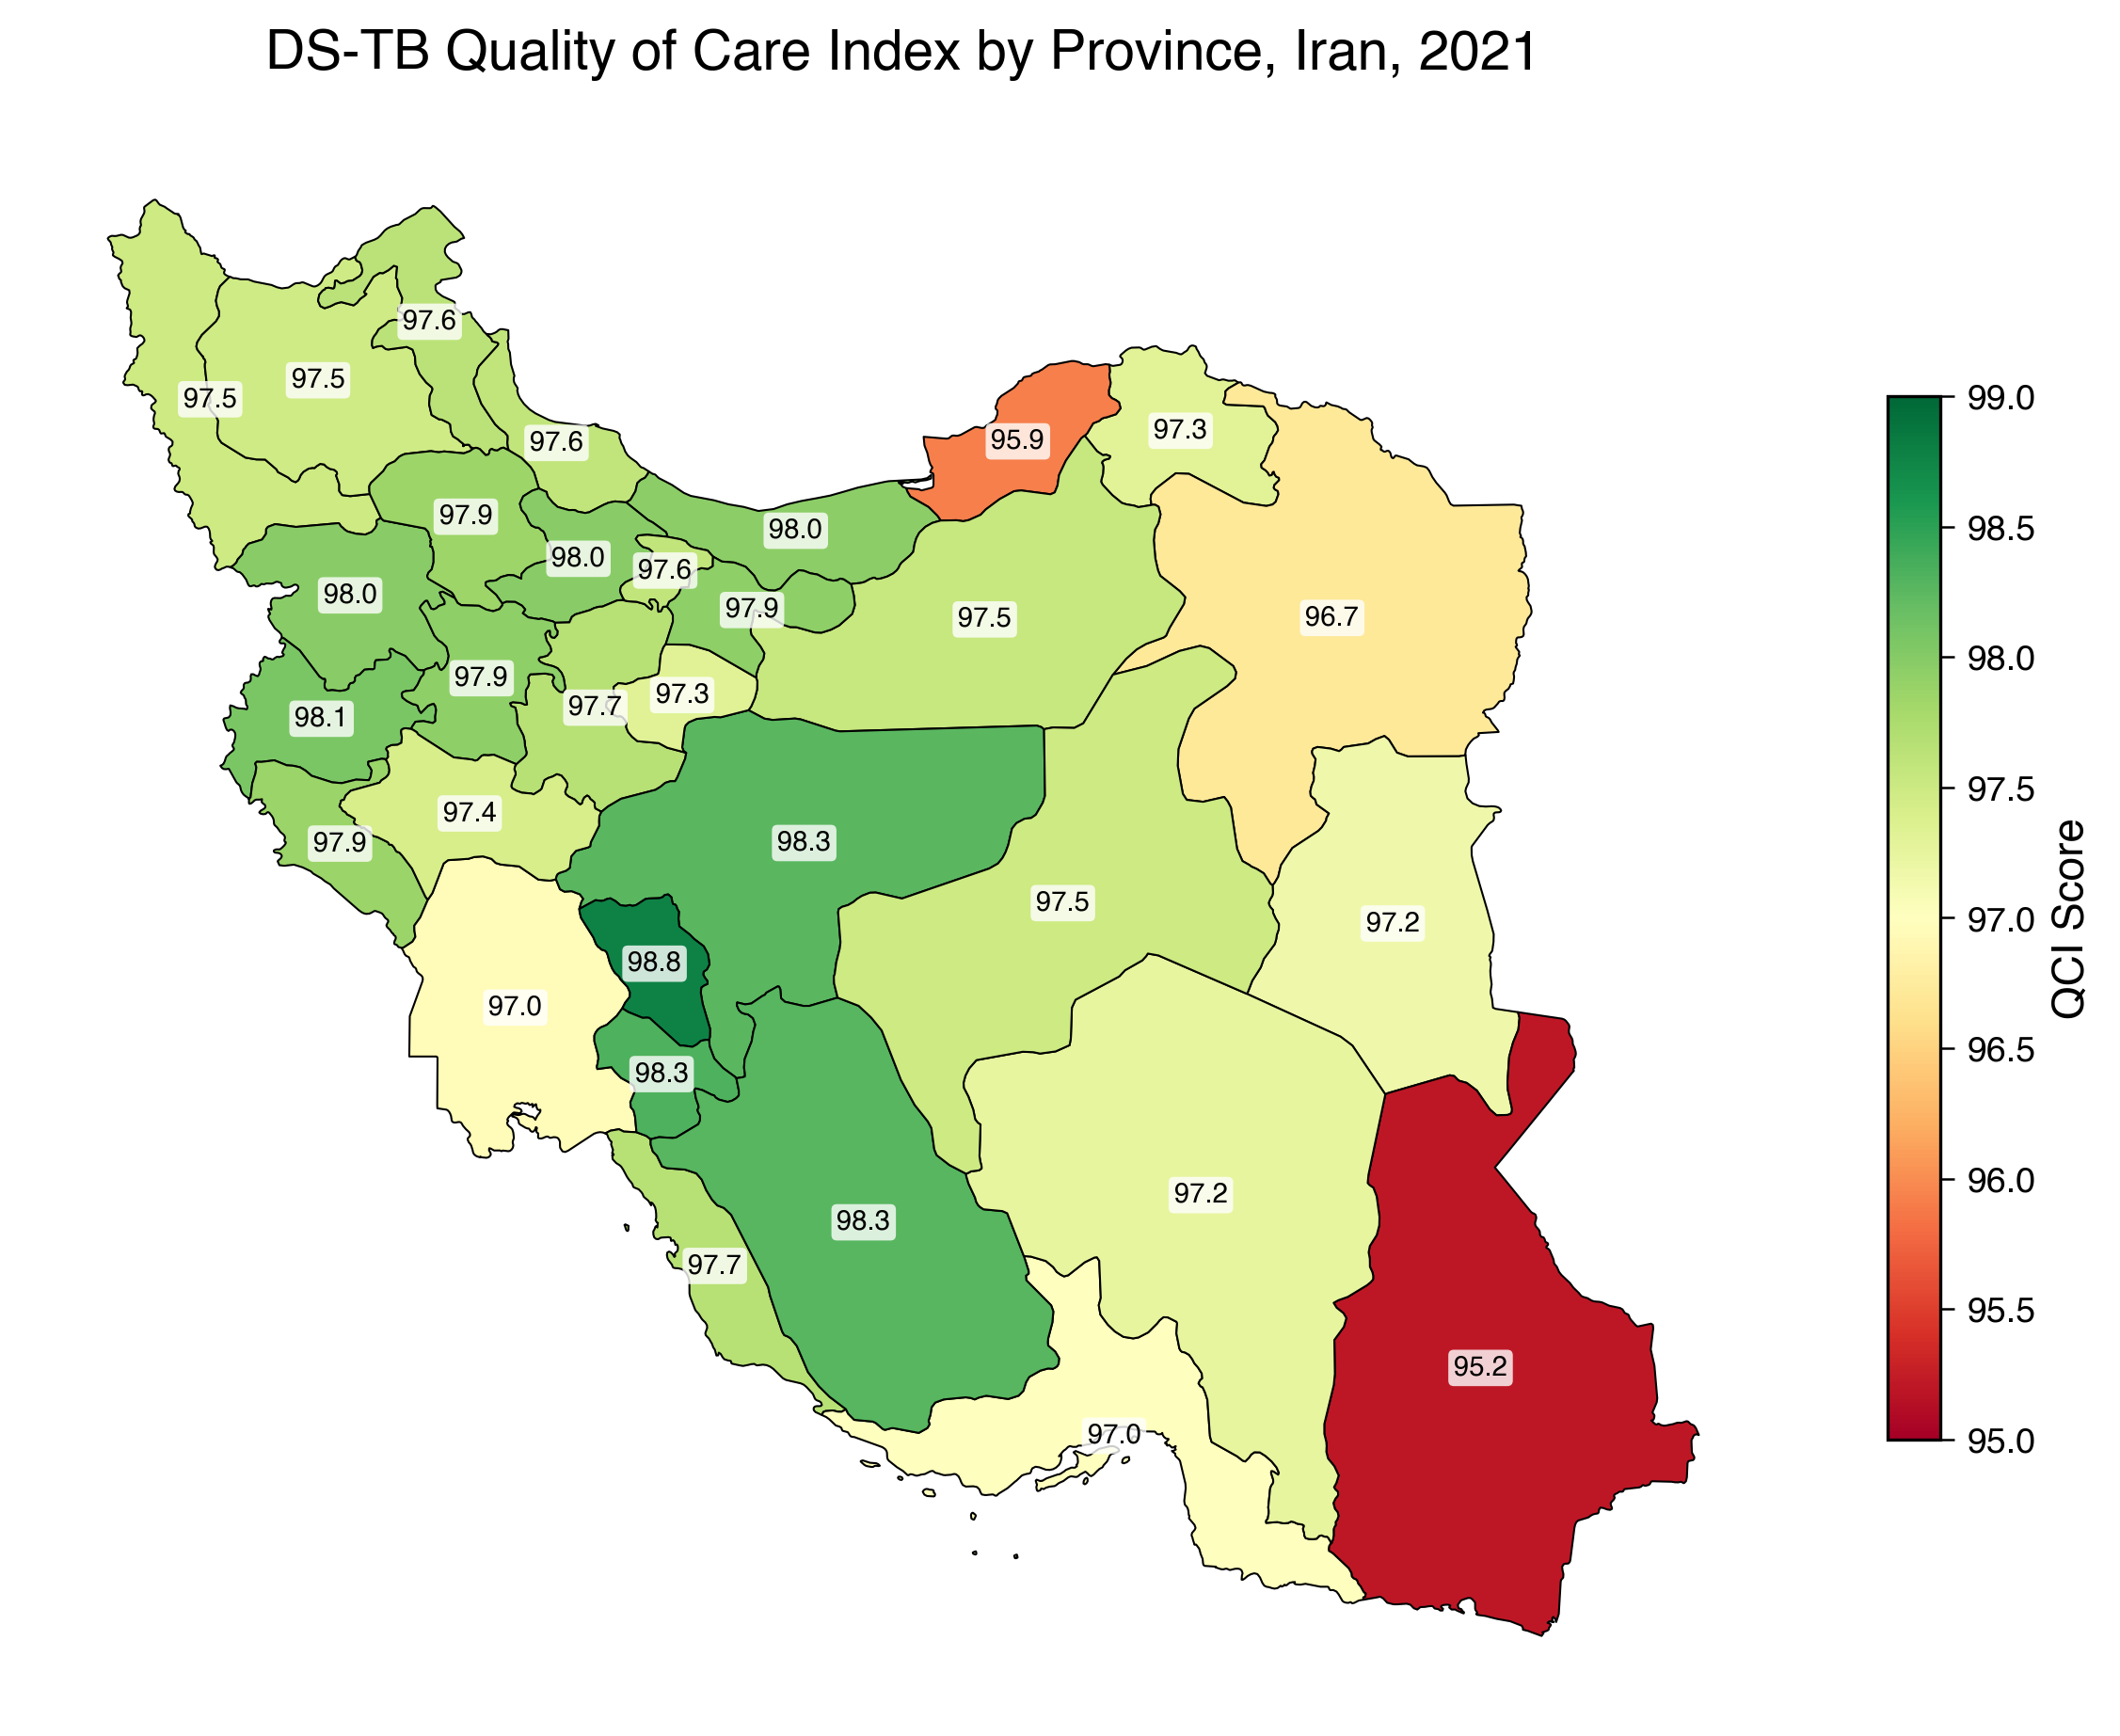
\includegraphics[width=0.85\textwidth]{figure1a_choropleth_2021.png}

\vspace{1em}

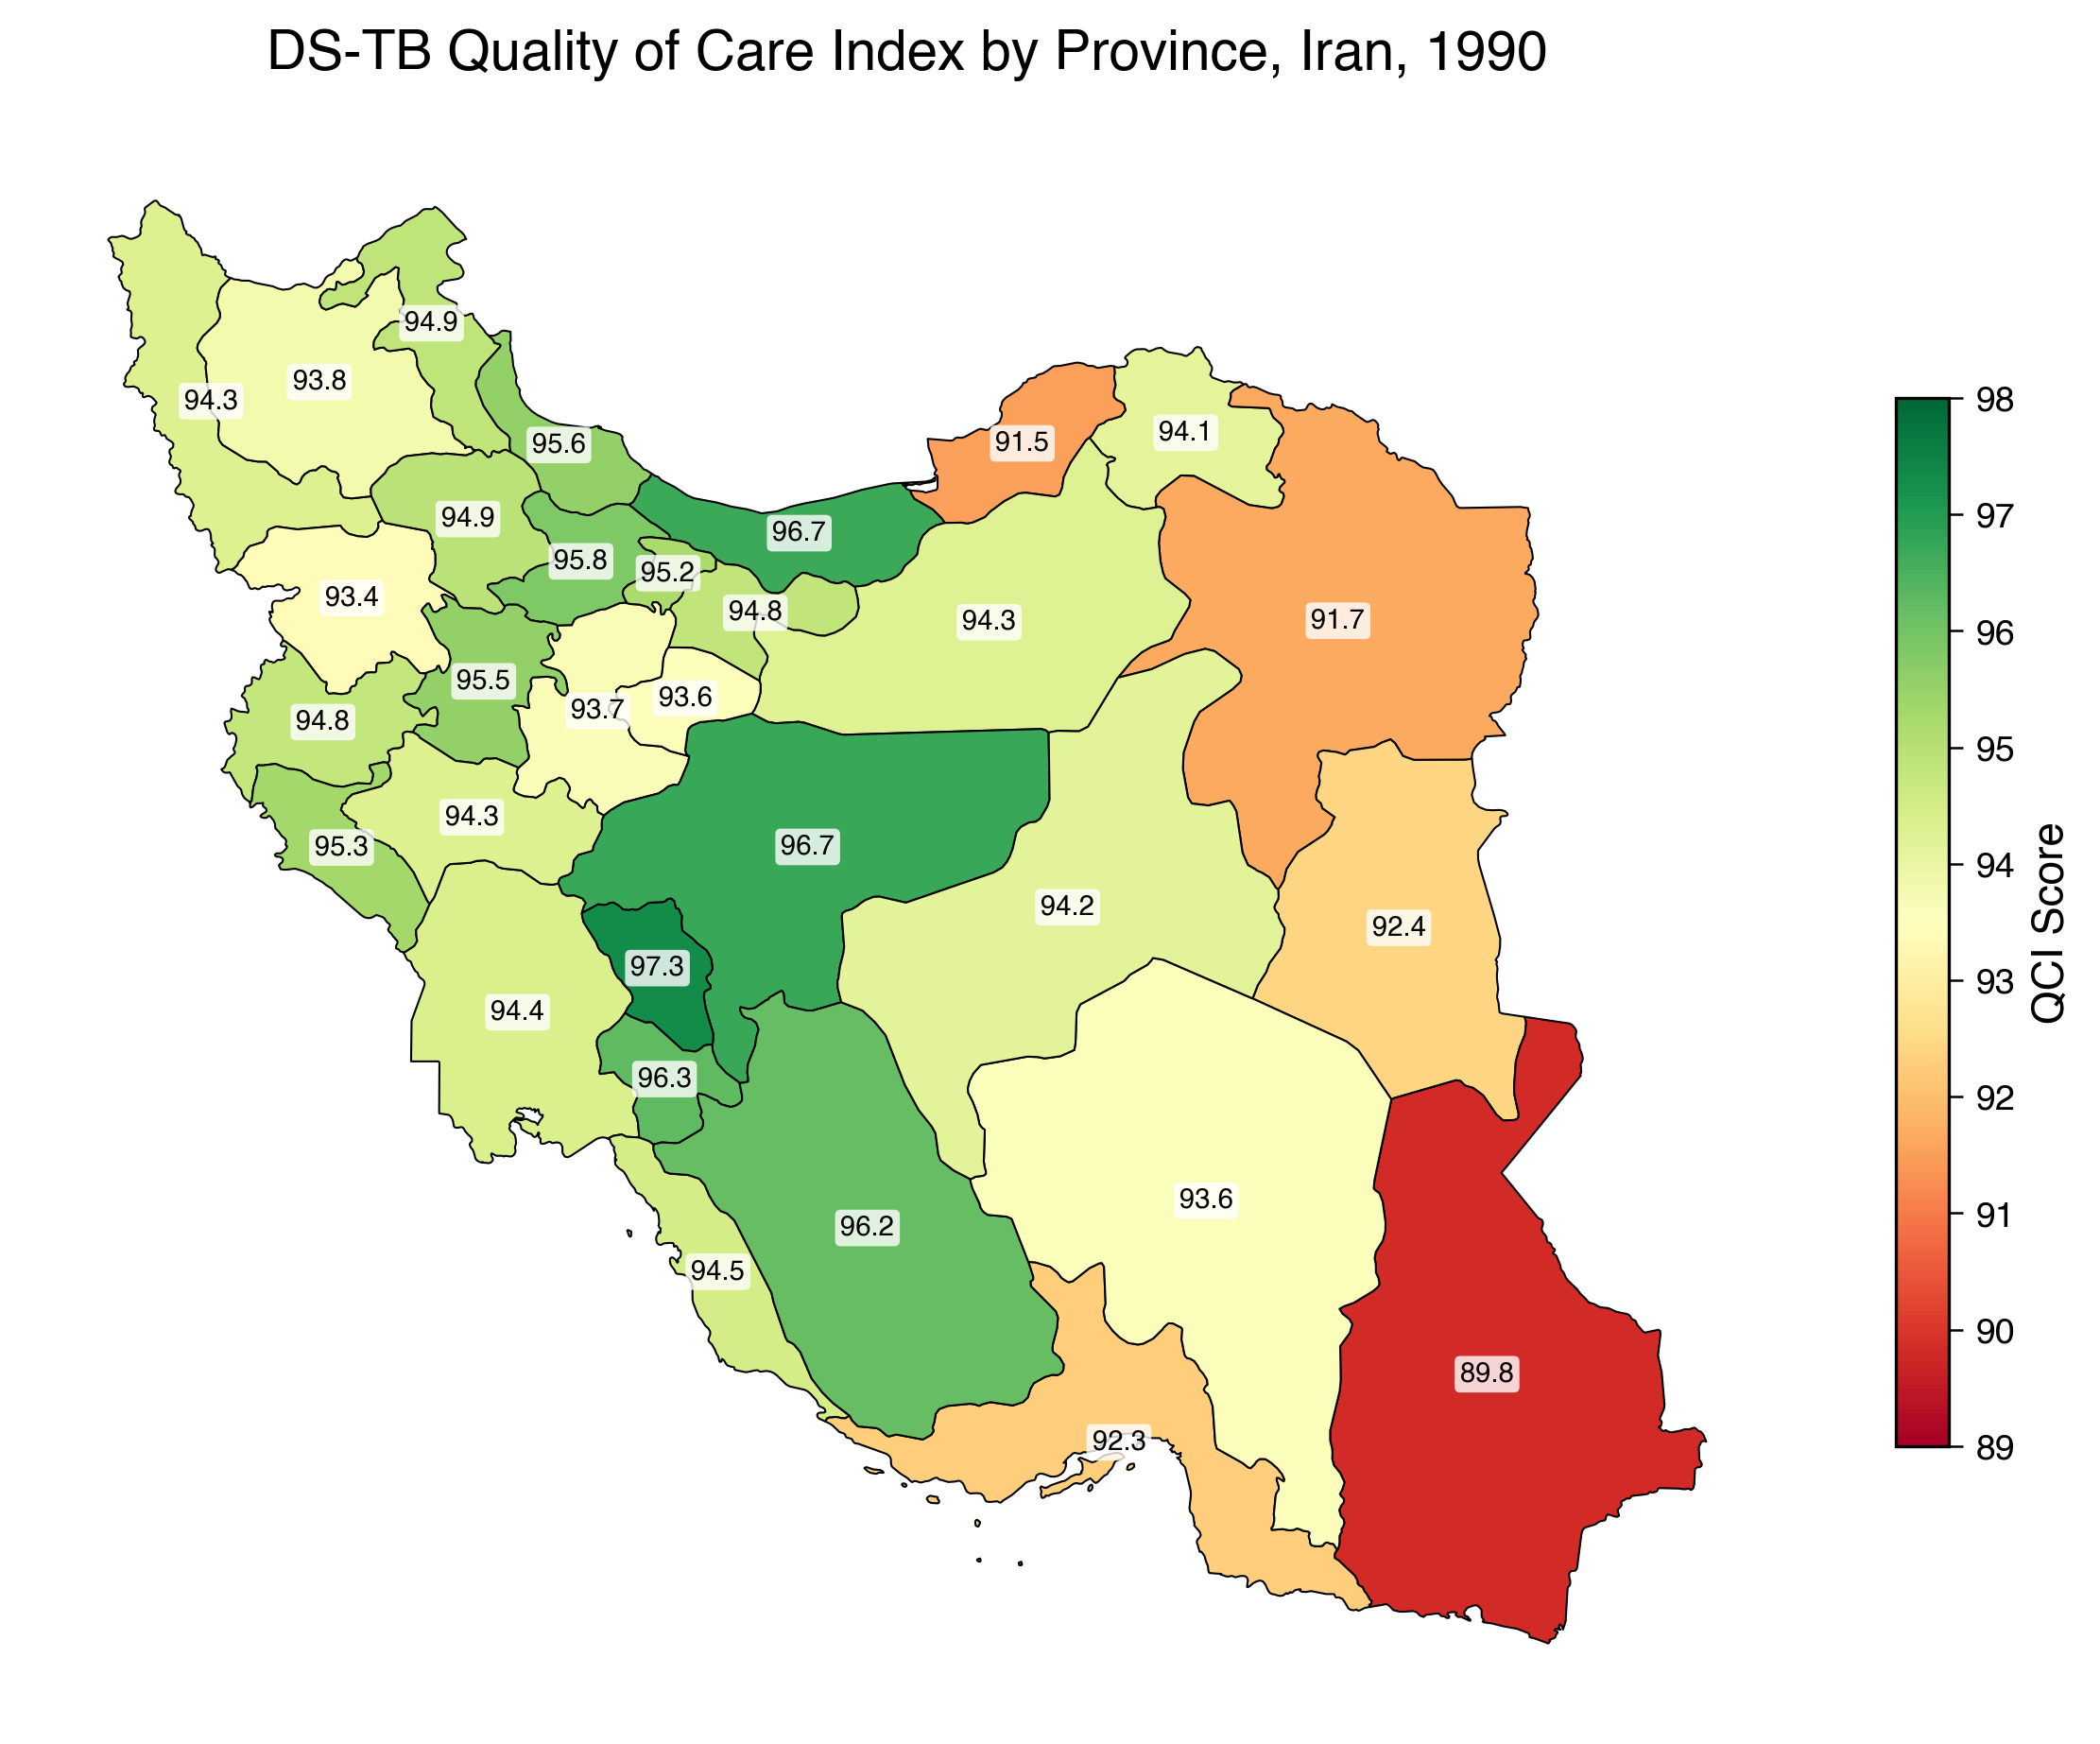
\includegraphics[width=0.85\textwidth]{figure1b_choropleth_1990.png}

\vspace{1em}

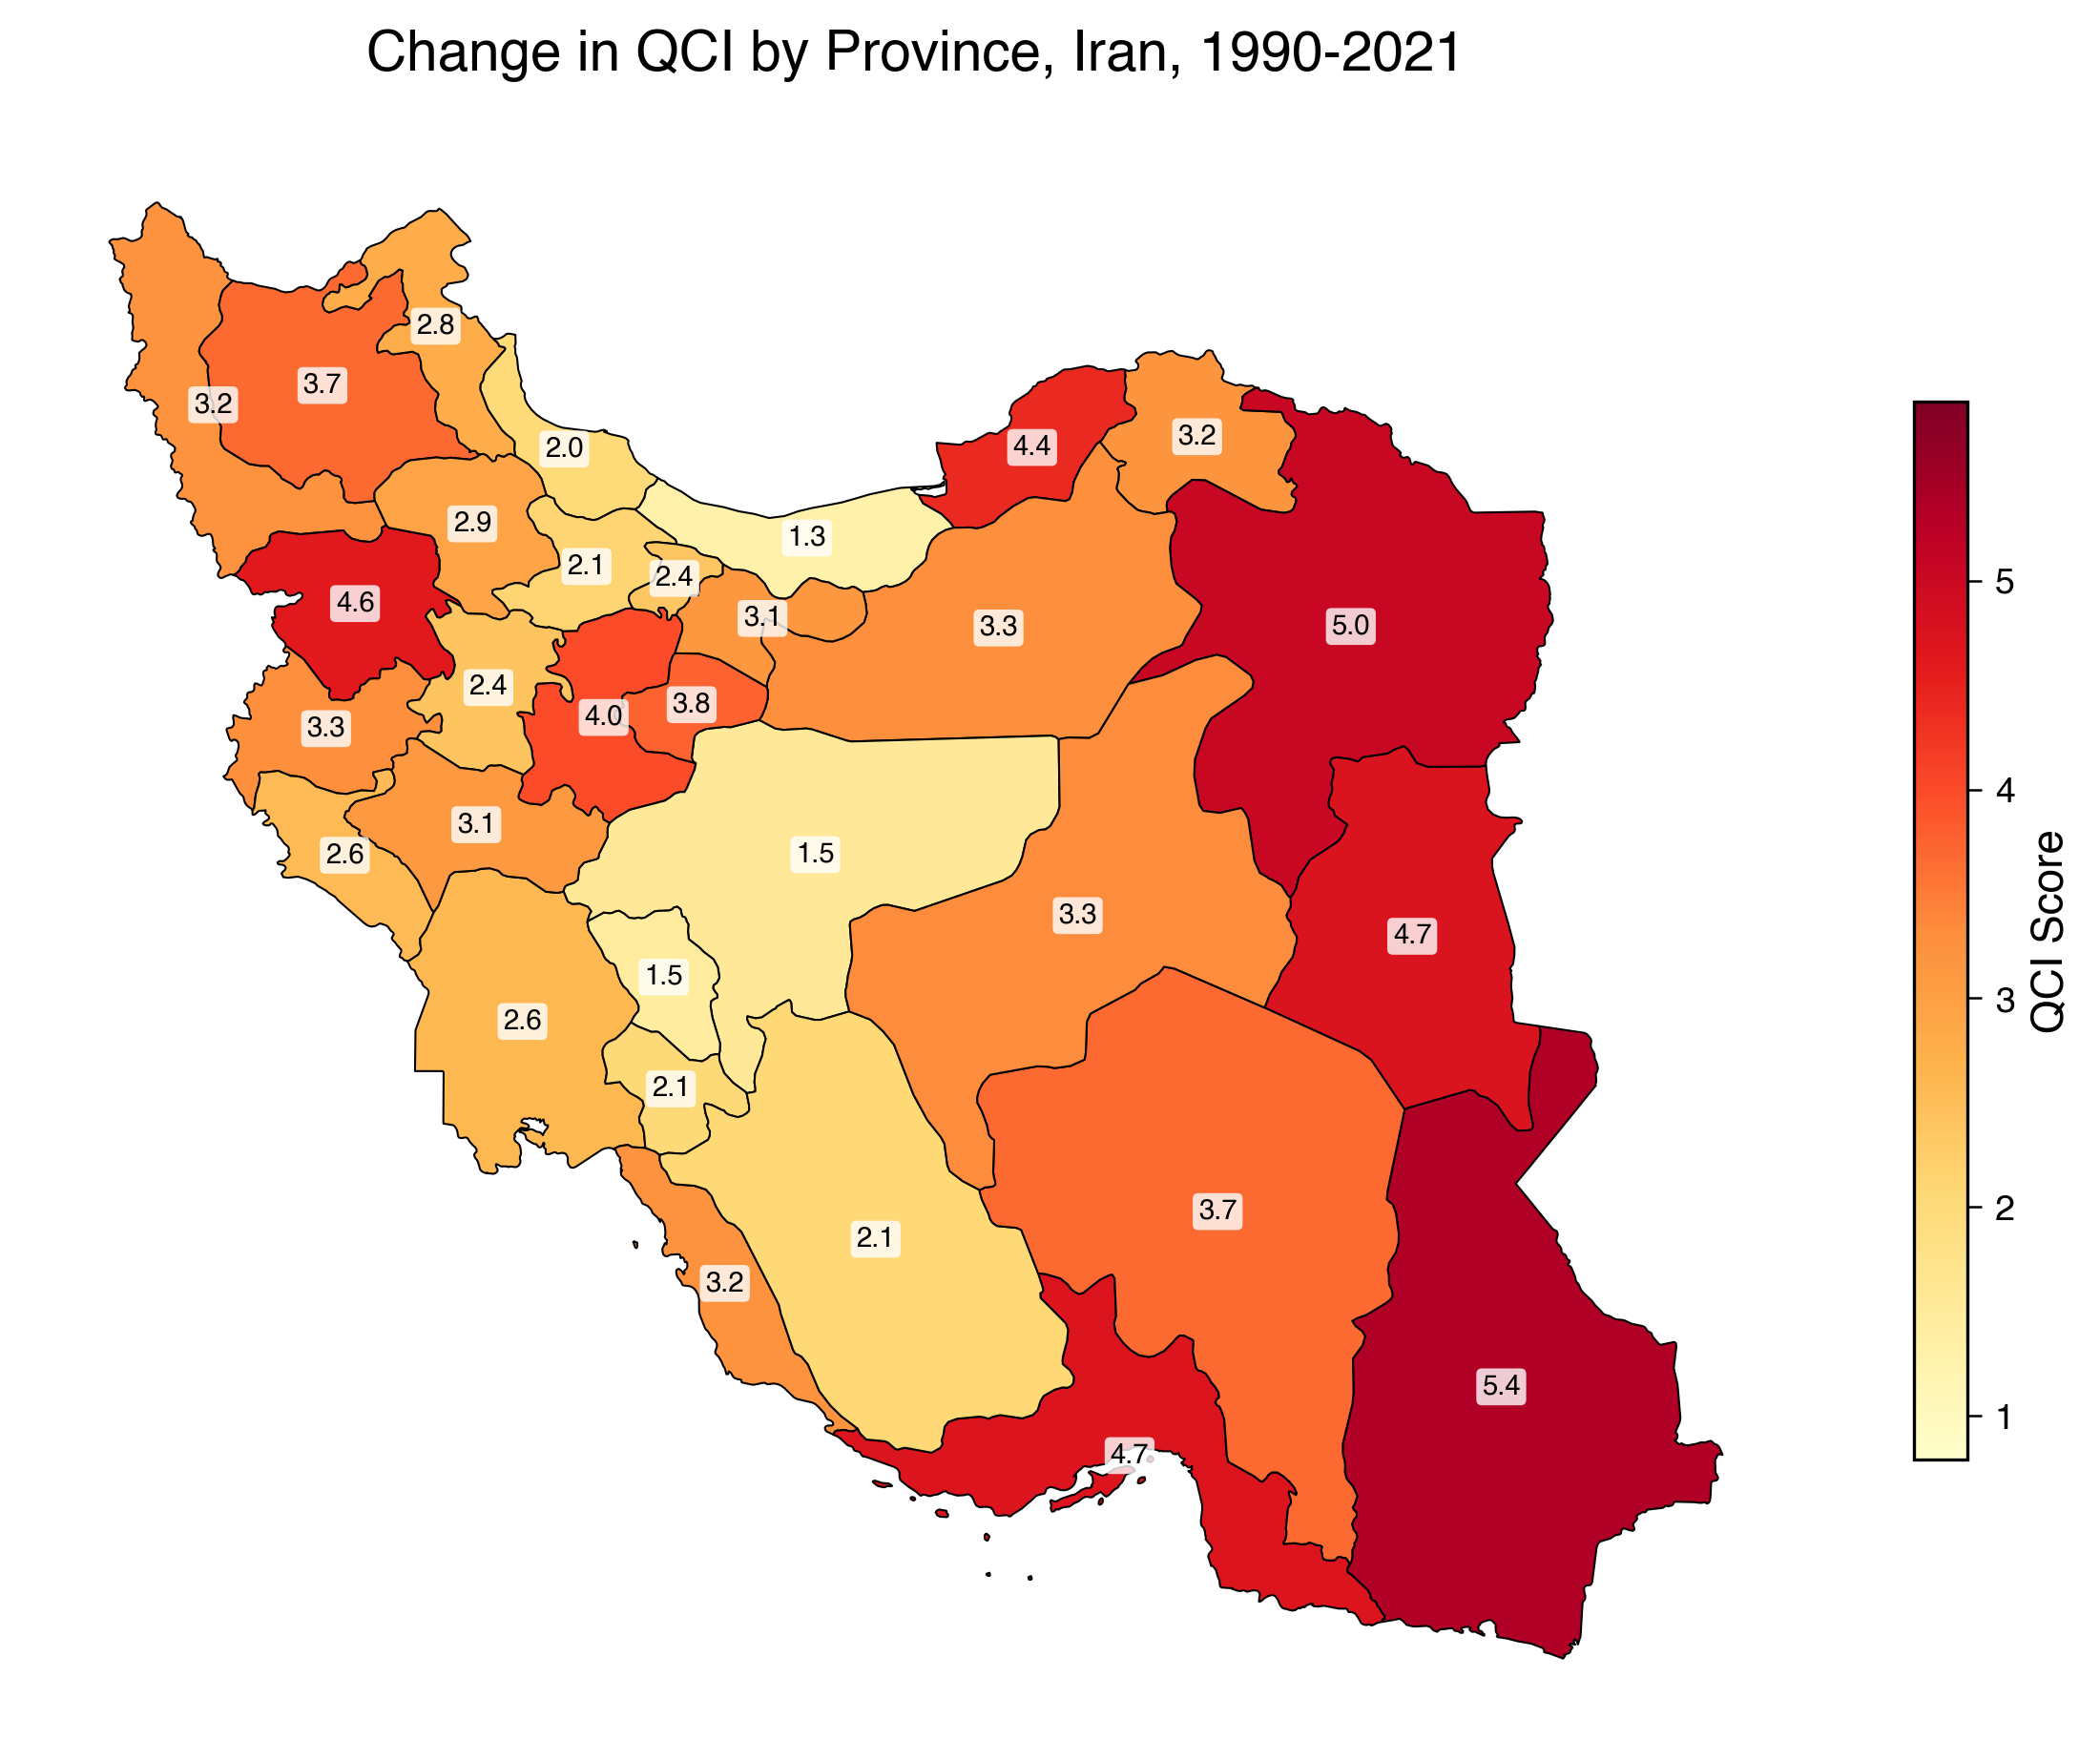
\includegraphics[width=0.85\textwidth]{figure1c_choropleth_change.png}
\caption{Choropleth maps of DS-TB QCI by province, Iran, 2021 (Panel A), 1990 (Panel B), and change 1990--2021 (Panel C). Higher QCI (darker green) indicates better care quality. All provinces transitioned from lower (yellow-green) to higher (dark green) QCI between 1990 and 2021, with the southeastern provinces showing the largest gains.}
\label{fig:figure1}
\end{figure}

\clearpage

\begin{figure}[htbp]
\centering
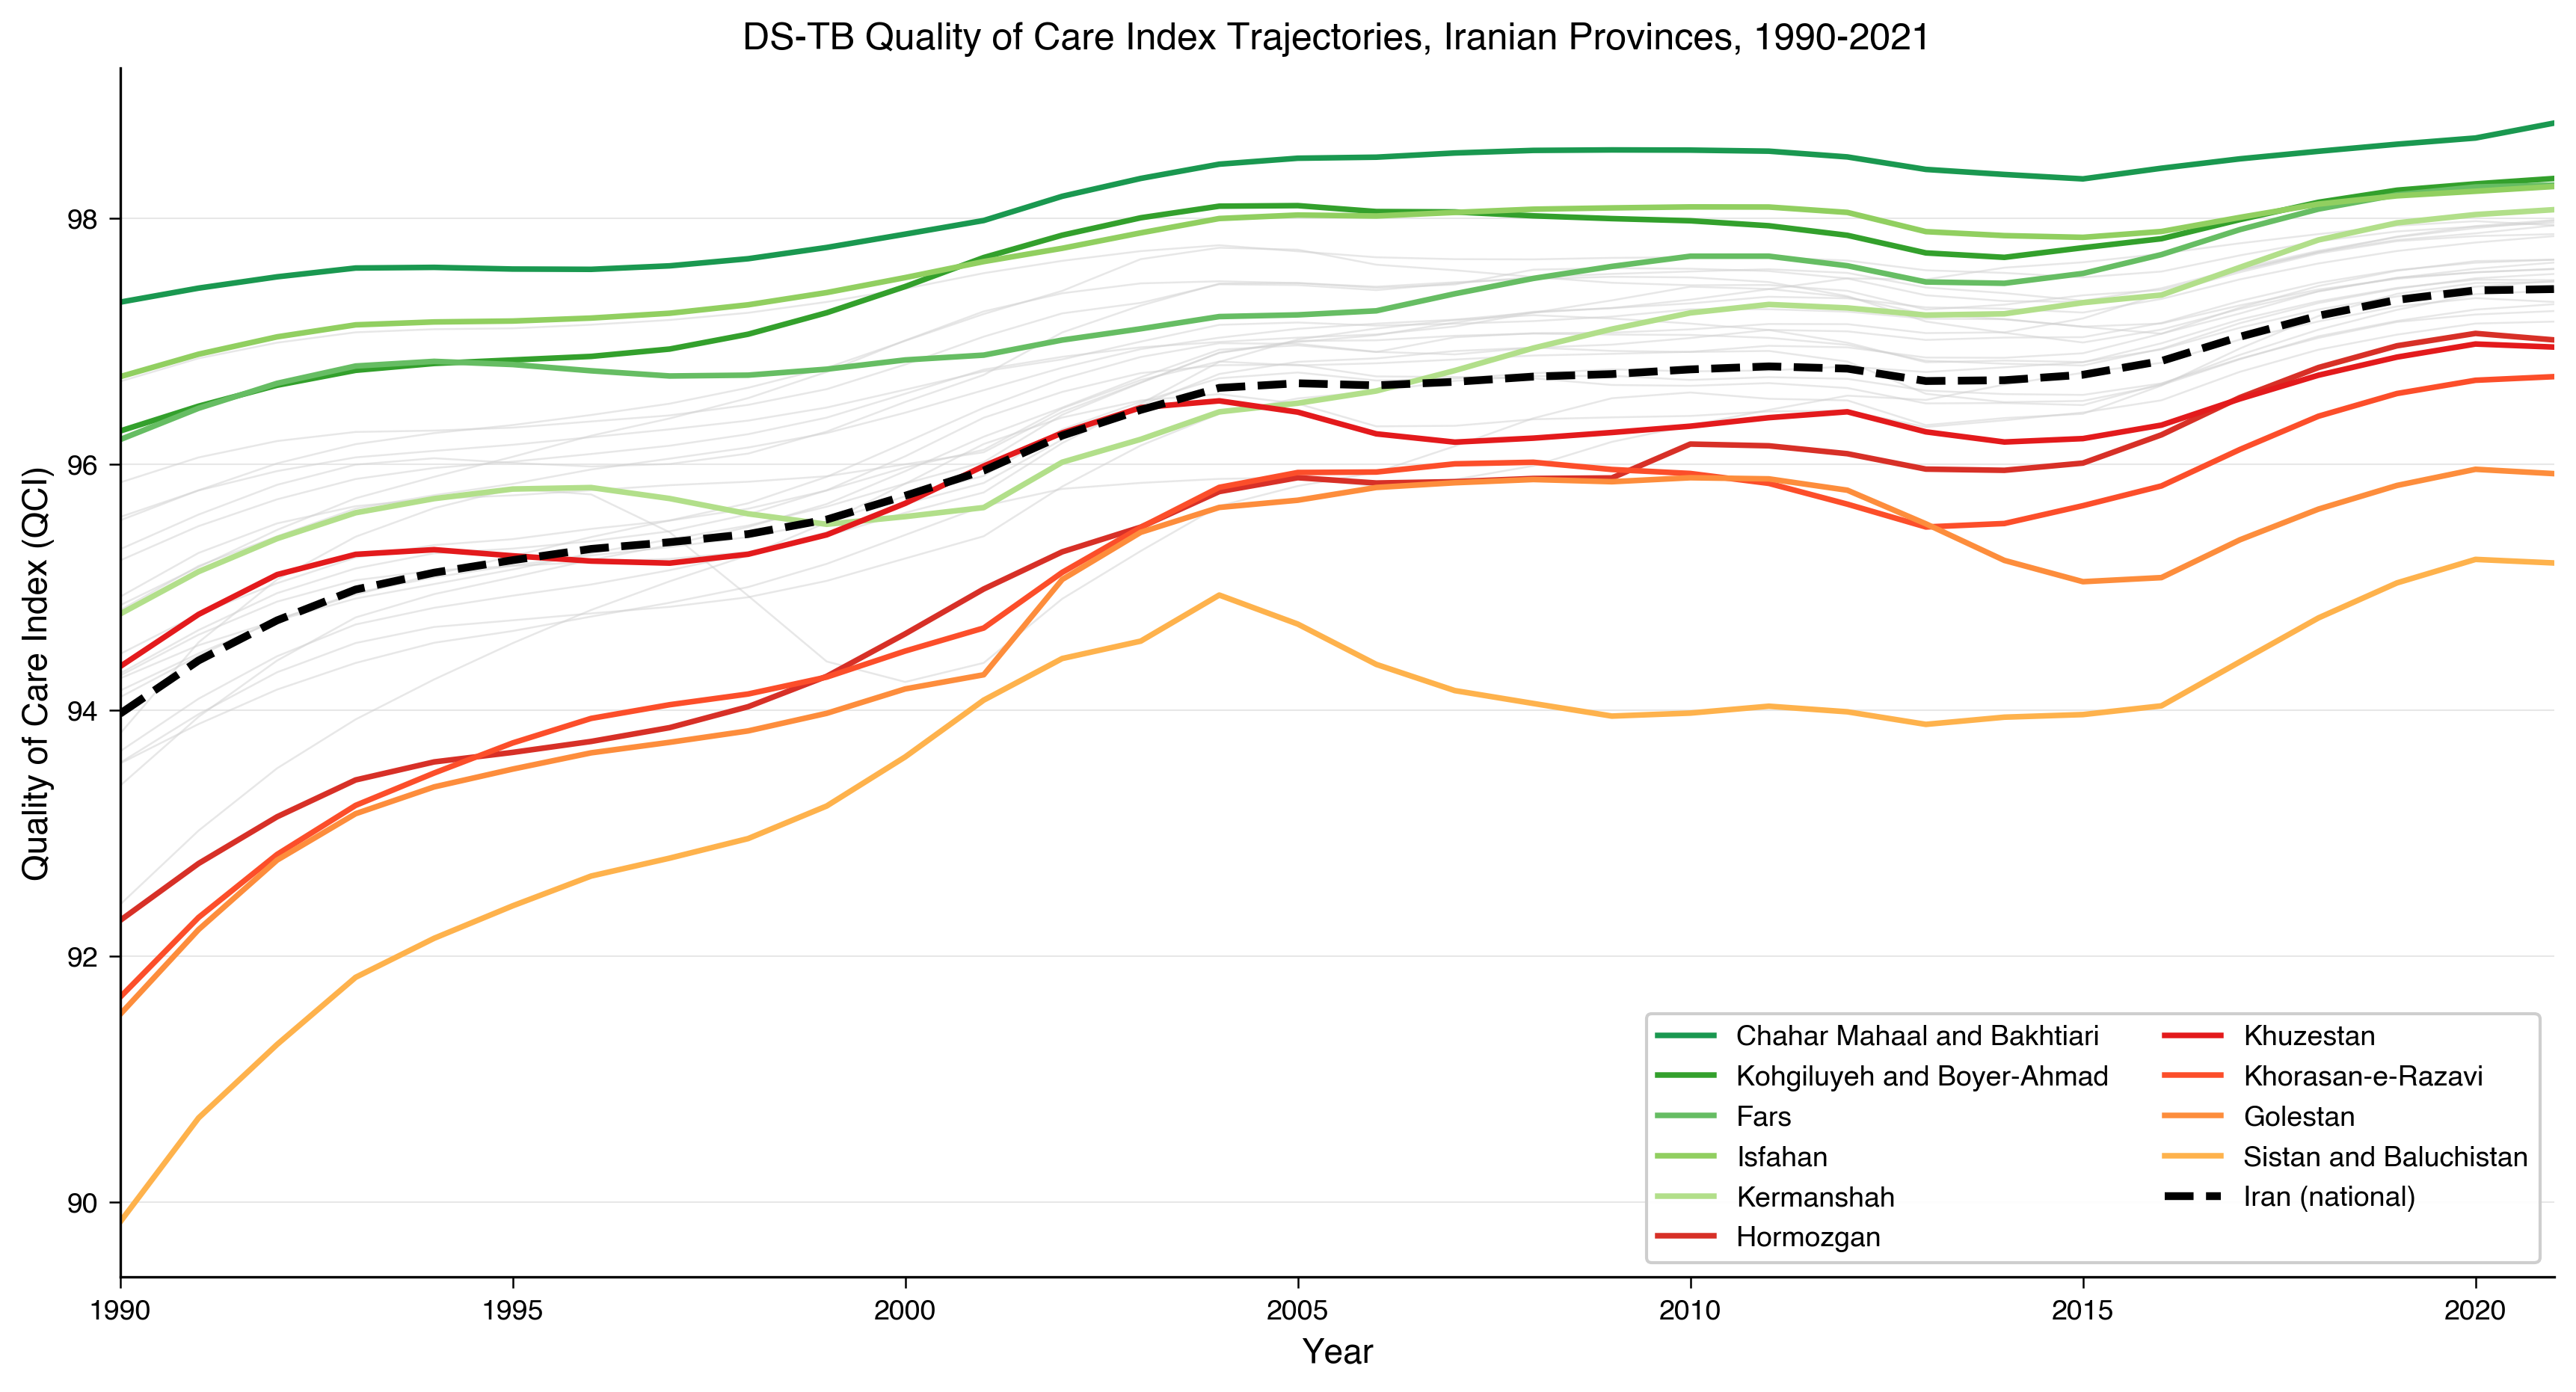
\includegraphics[width=\textwidth]{figure2_provincial_timeseries.png}
\caption{QCI trajectories for all 31 Iranian provinces, 1990--2021. Top five provinces (green), bottom five provinces (red), and remaining provinces (grey). Black dashed line indicates Iran's national QCI. All provinces converged toward higher values over the study period.}
\label{fig:figure2}
\end{figure}

\clearpage

\begin{figure}[htbp]
\centering
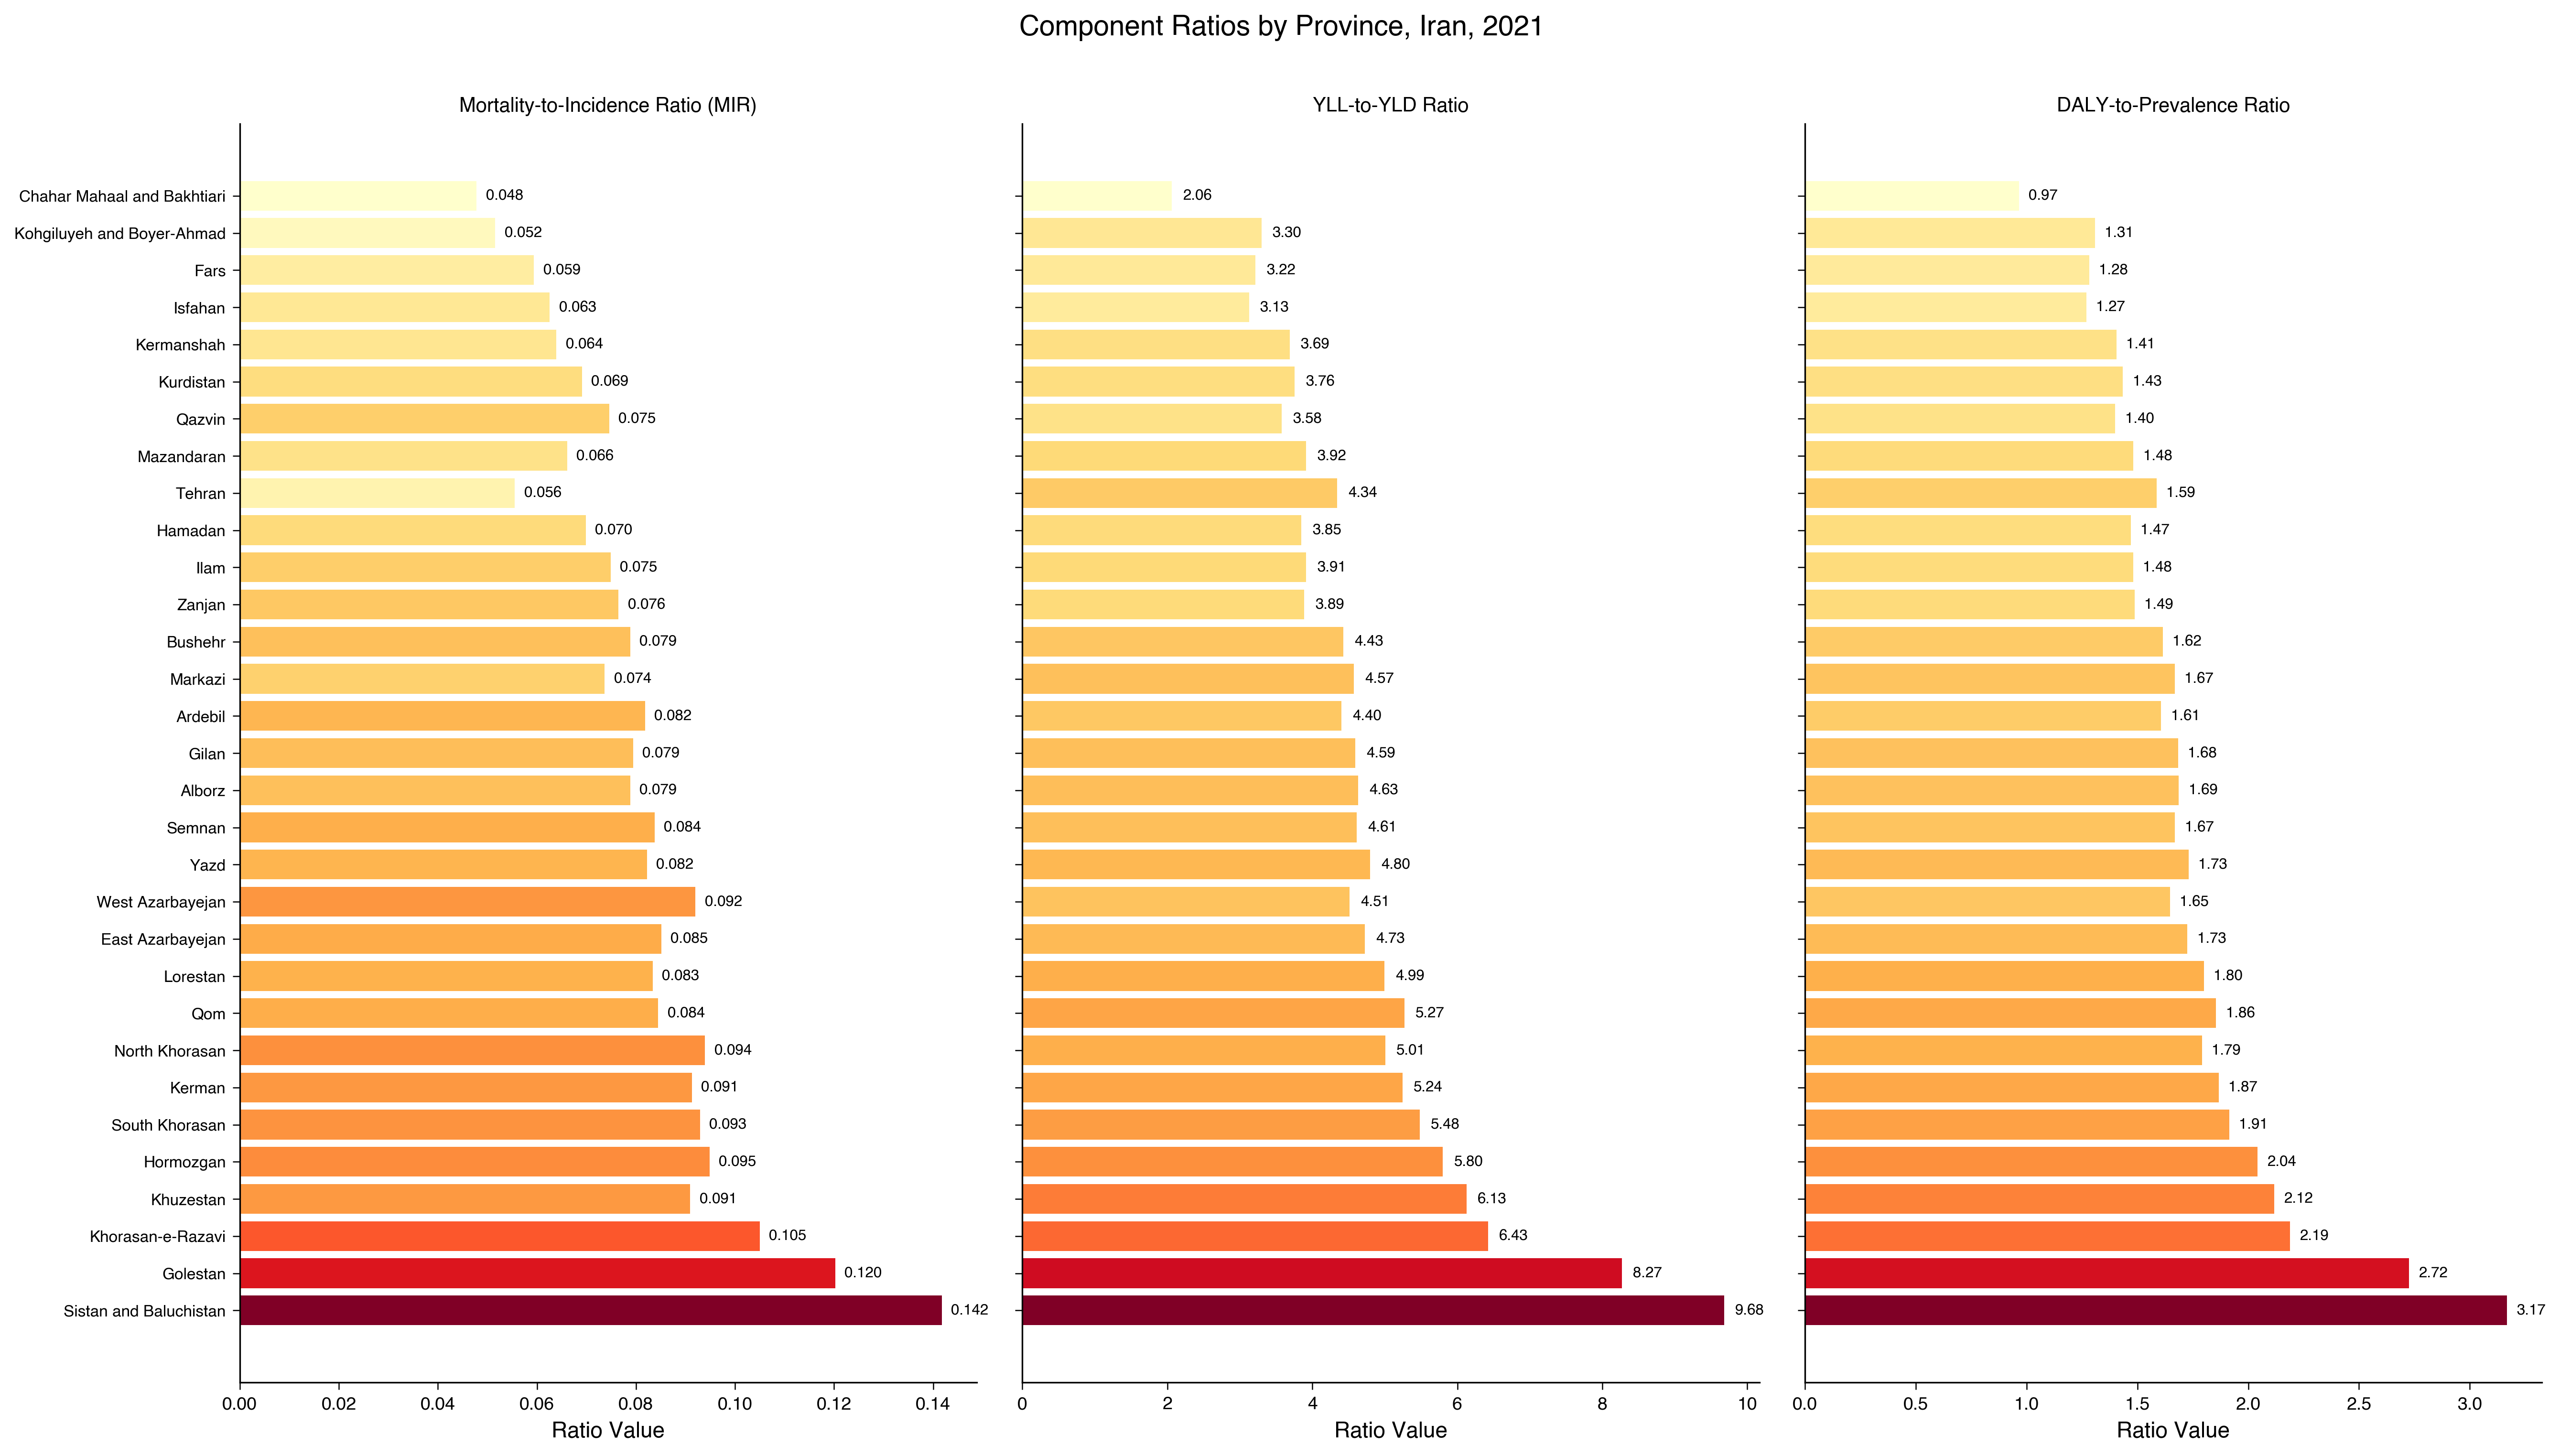
\includegraphics[width=\textwidth]{figure3_component_heatmap.png}
\caption{Component ratios (MIR, YLL/YLD, DALY/Prevalence) by province, Iran, 2021. Provinces sorted by overall QCI (ascending from top). Sistan and Baluchistan has the highest (worst) values across all three components.}
\label{fig:figure3}
\end{figure}

\clearpage

\begin{figure}[htbp]
\centering
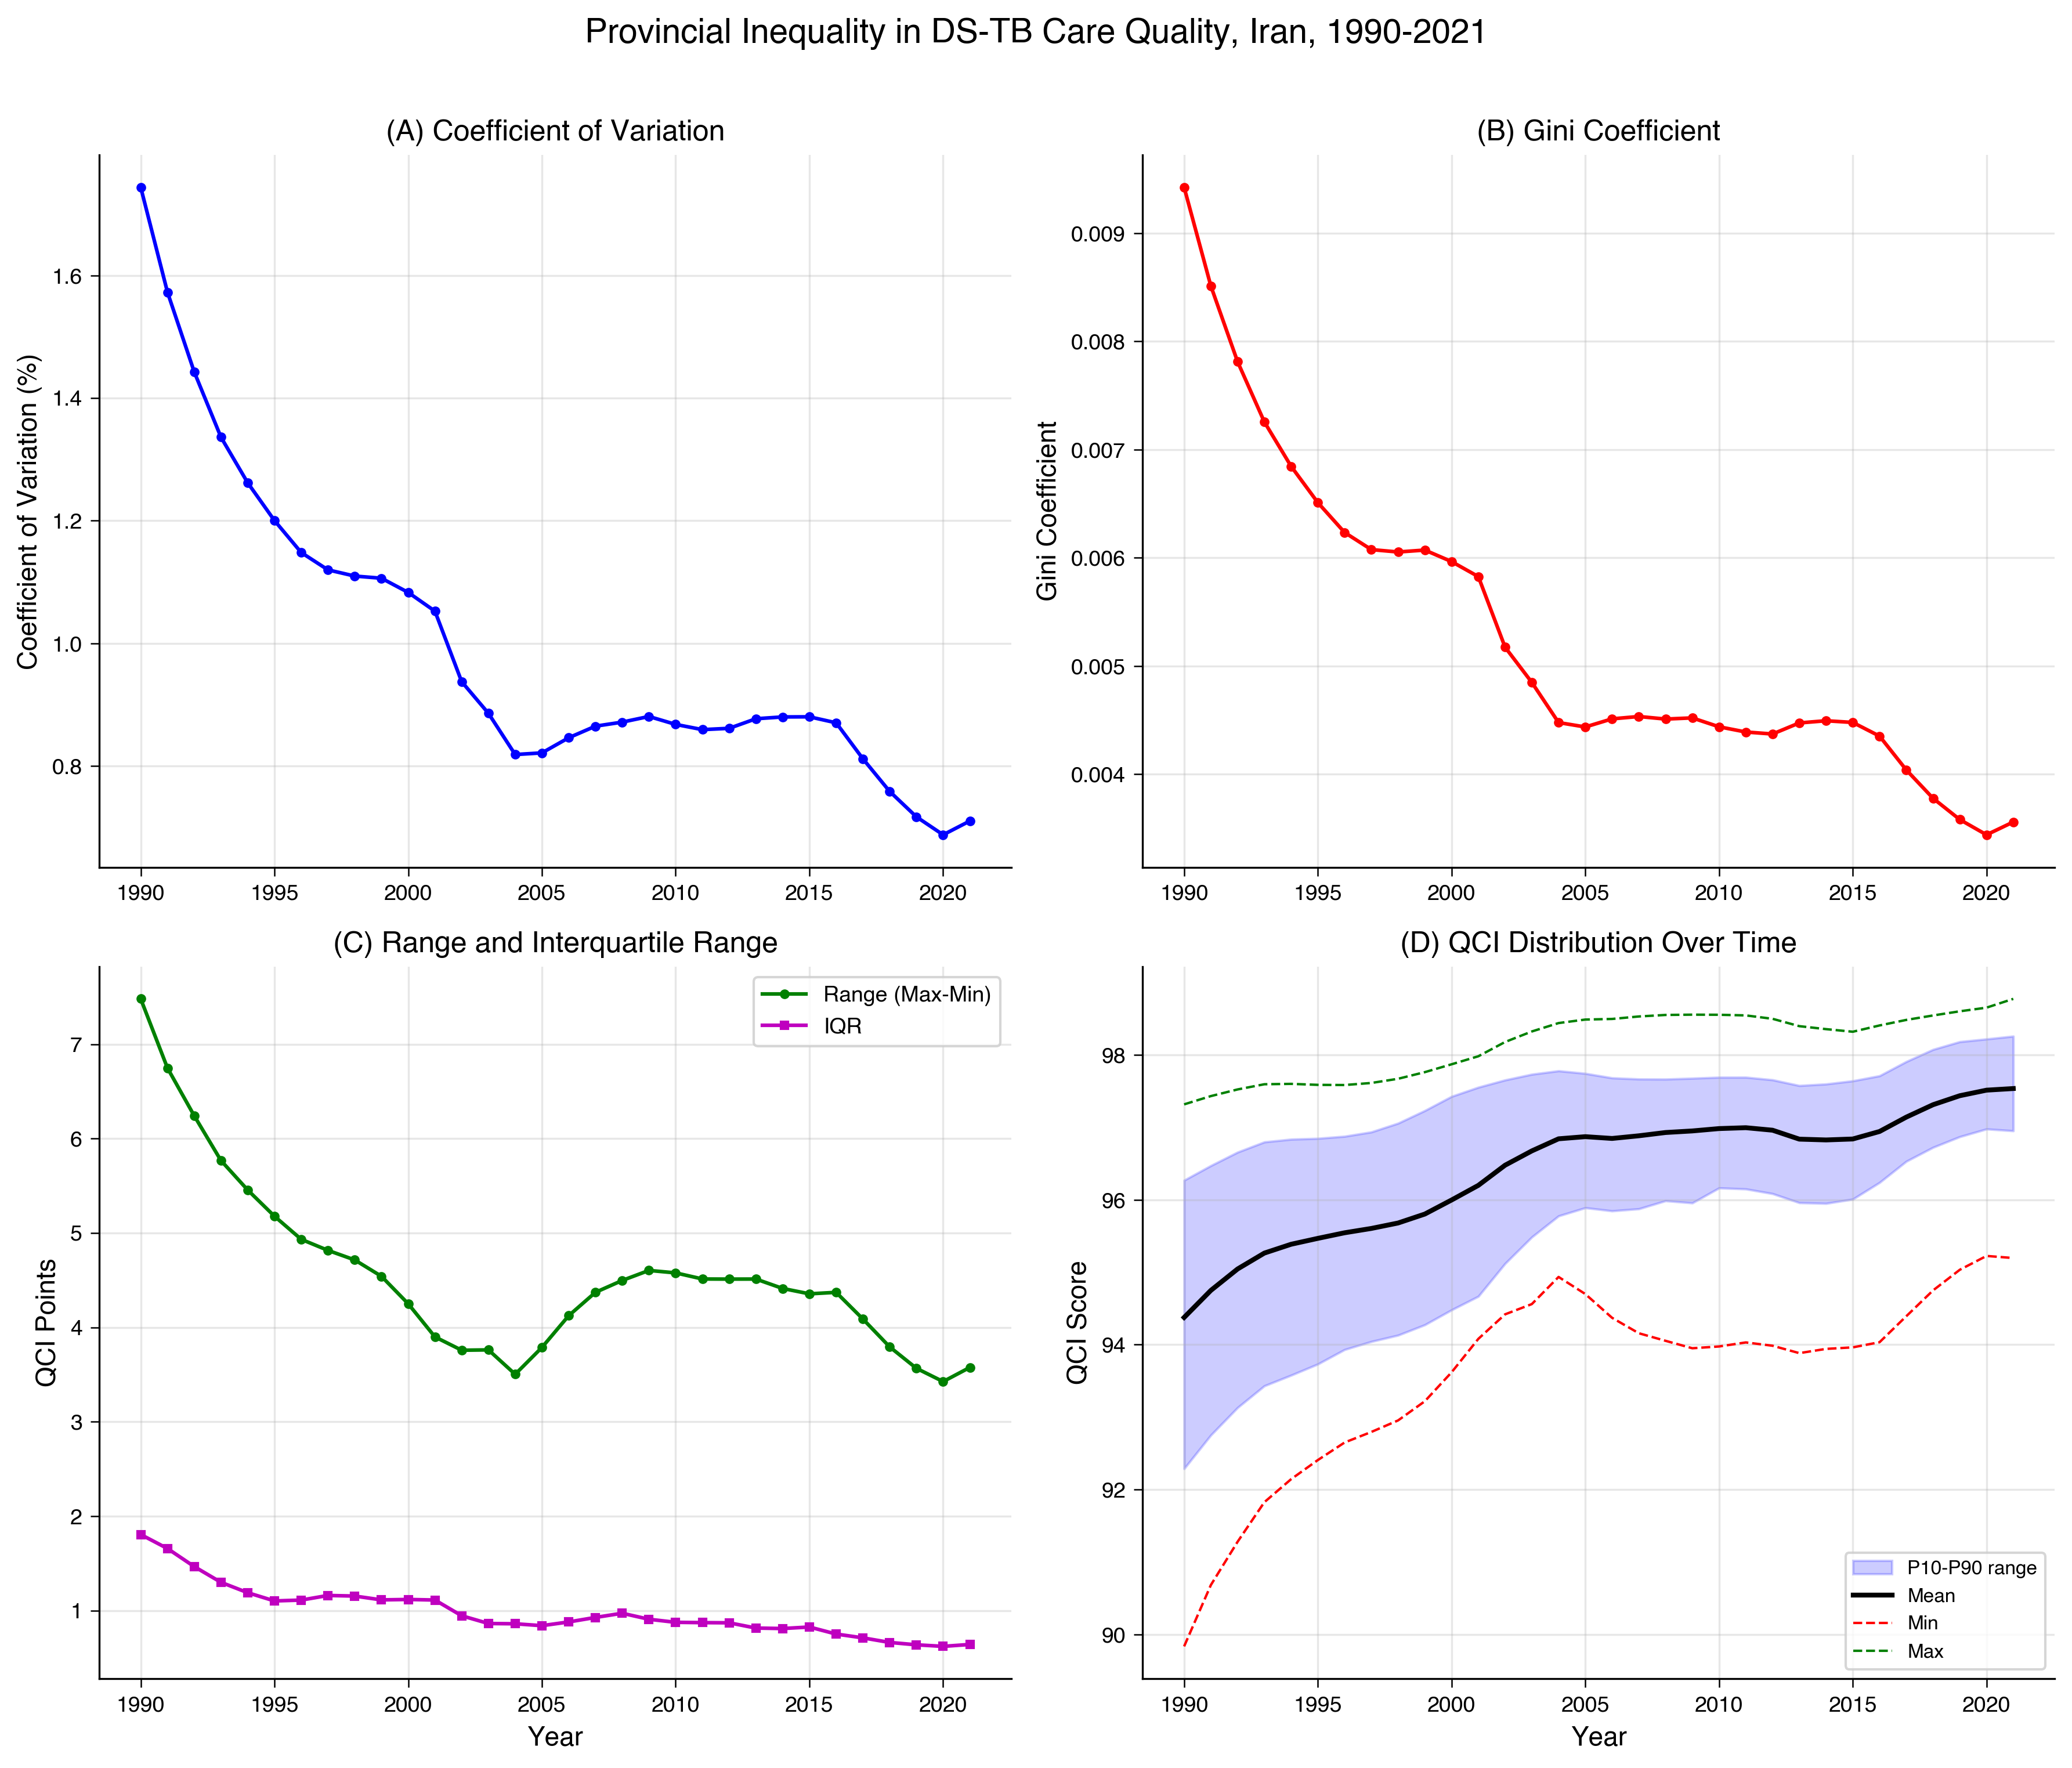
\includegraphics[width=\textwidth]{figure4_inequality_metrics.png}
\caption{Provincial inequality metrics over time, 1990--2021: (A) coefficient of variation, (B) Gini coefficient, (C) range and IQR, (D) QCI distribution. All metrics show a declining trend, indicating convergence.}
\label{fig:figure4}
\end{figure}

\clearpage

\begin{figure}[htbp]
\centering
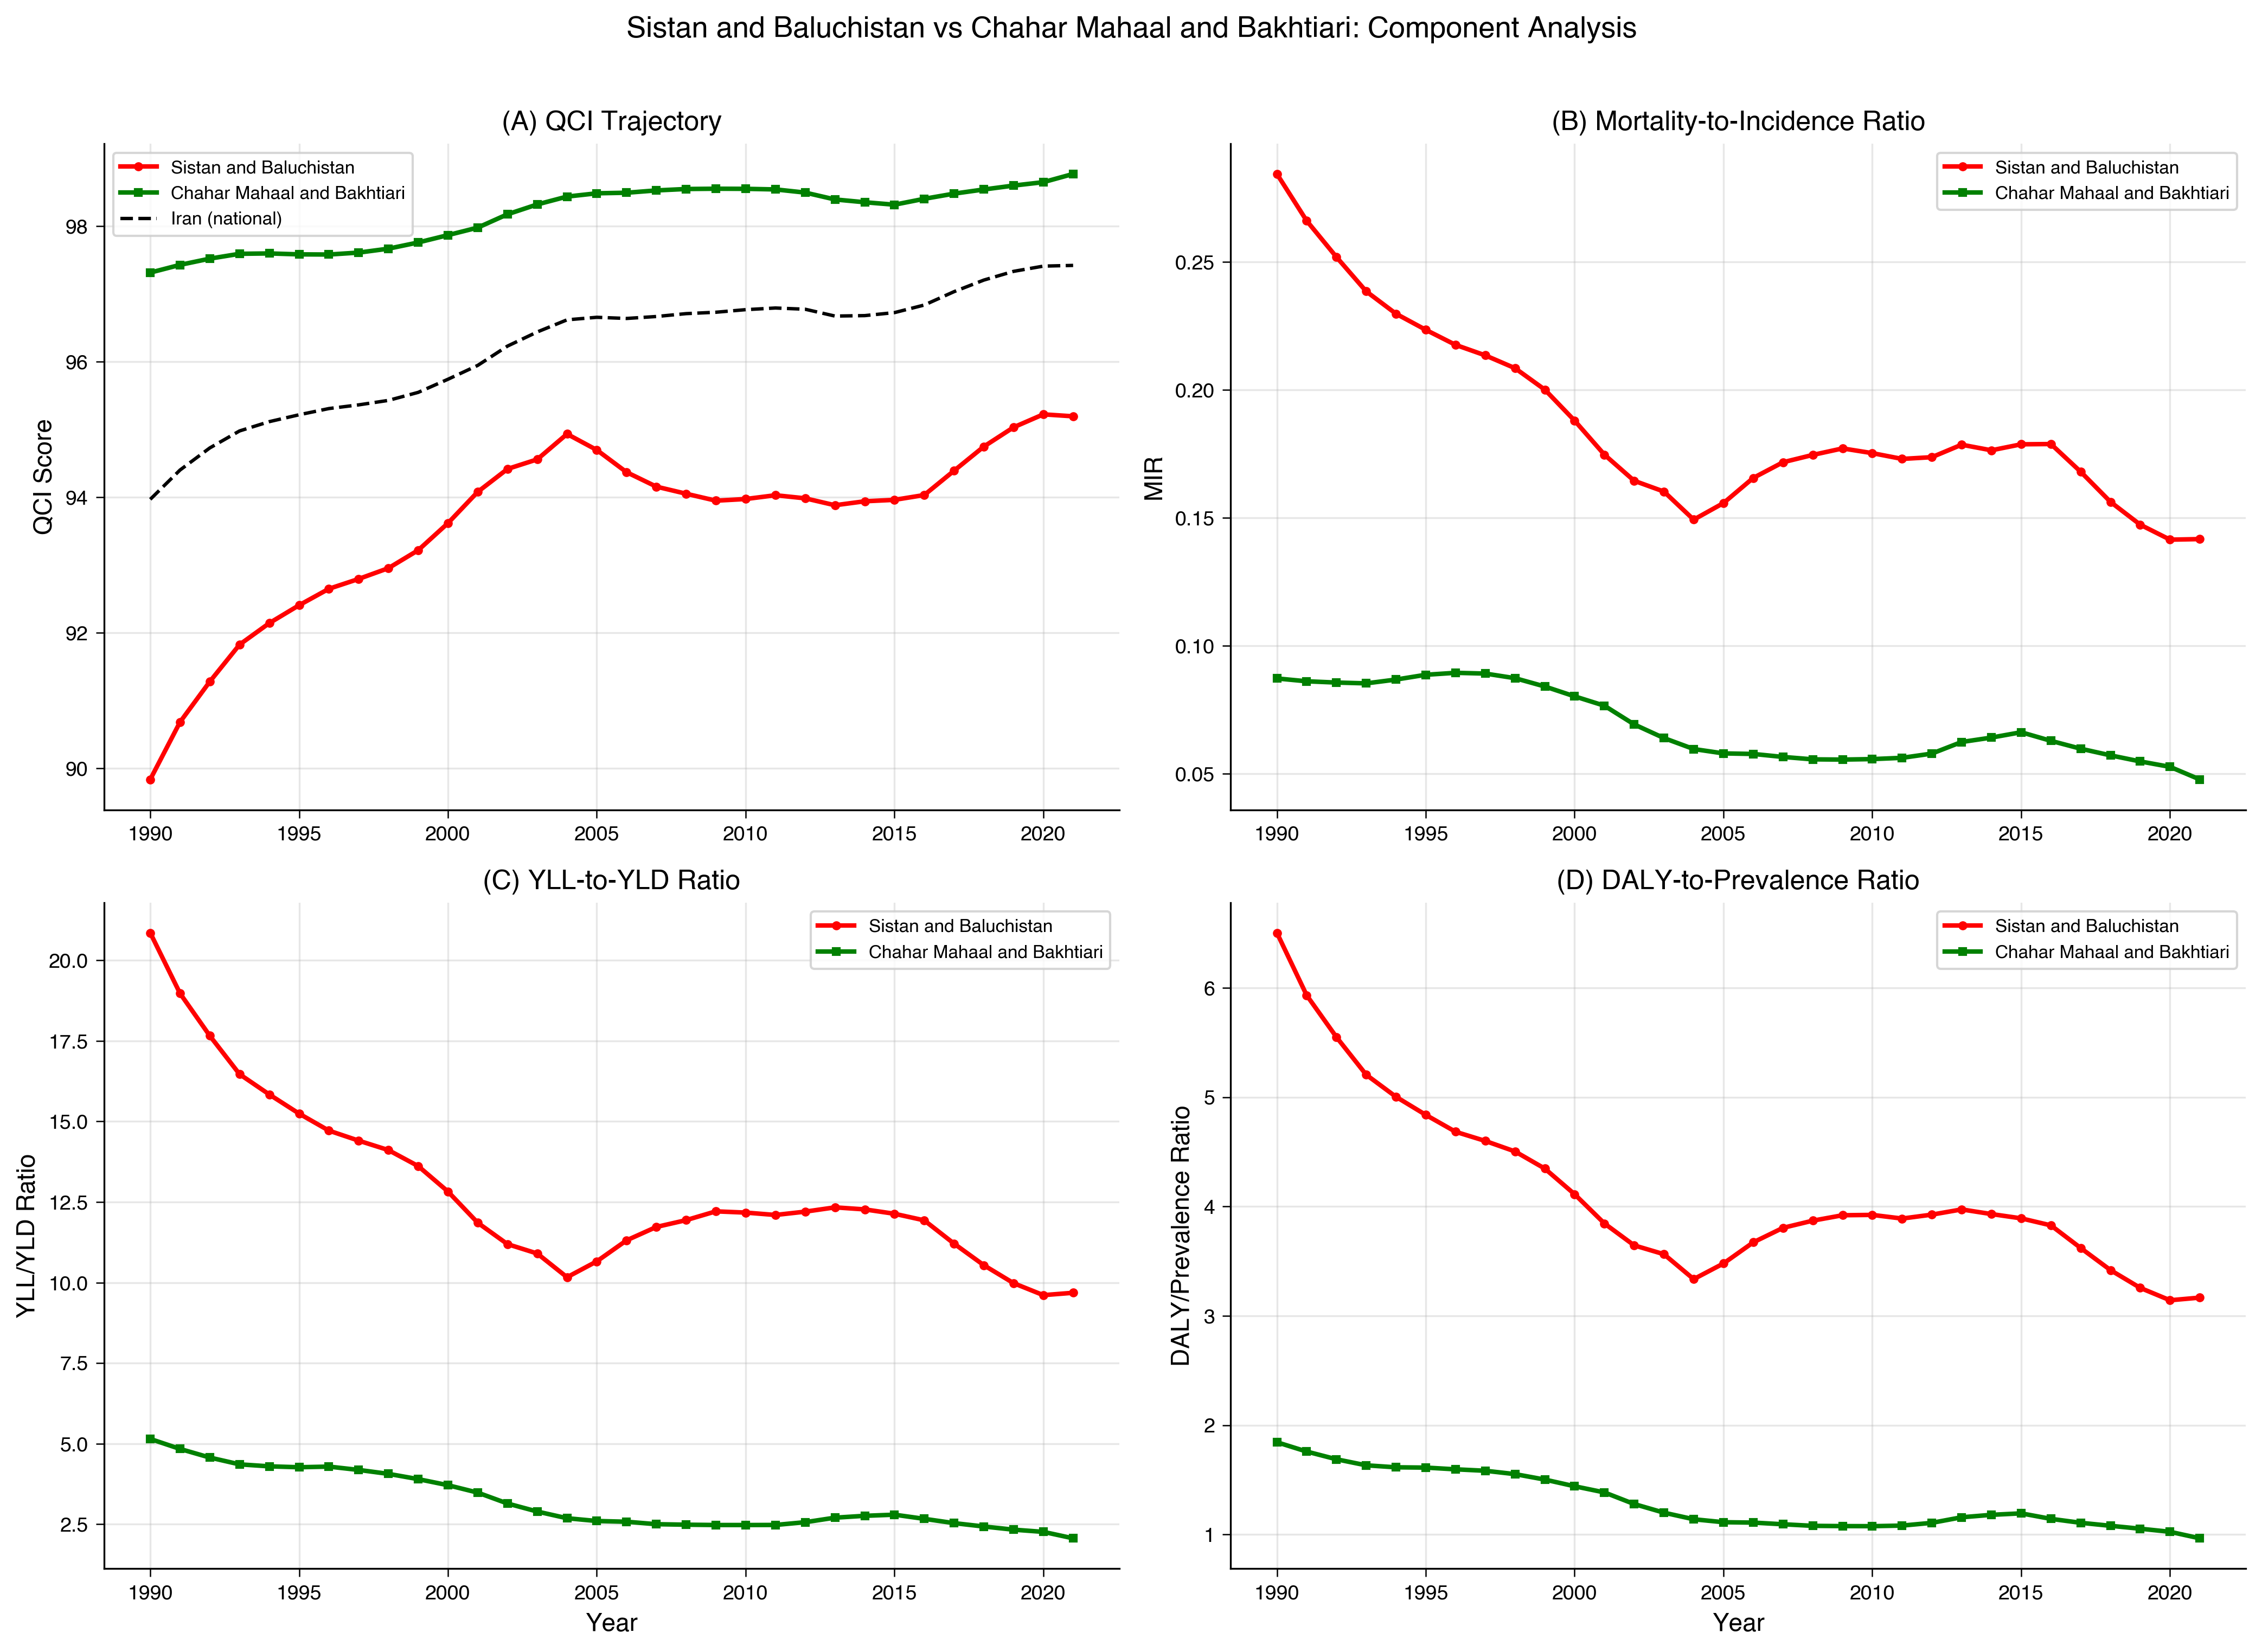
\includegraphics[width=\textwidth]{figure5_sistan_deep_dive.png}
\caption{Sistan and Baluchistan deep dive: (A) QCI trajectory compared with Chahar Mahaal and Bakhtiari and national average; (B) MIR over time; (C) YLL/YLD ratio over time; (D) DALY/Prevalence ratio over time. Despite persistent gaps, Sistan and Baluchistan shows consistent improvement across all components.}
\label{fig:figure5}
\end{figure}

\clearpage

\begin{figure}[htbp]
\centering
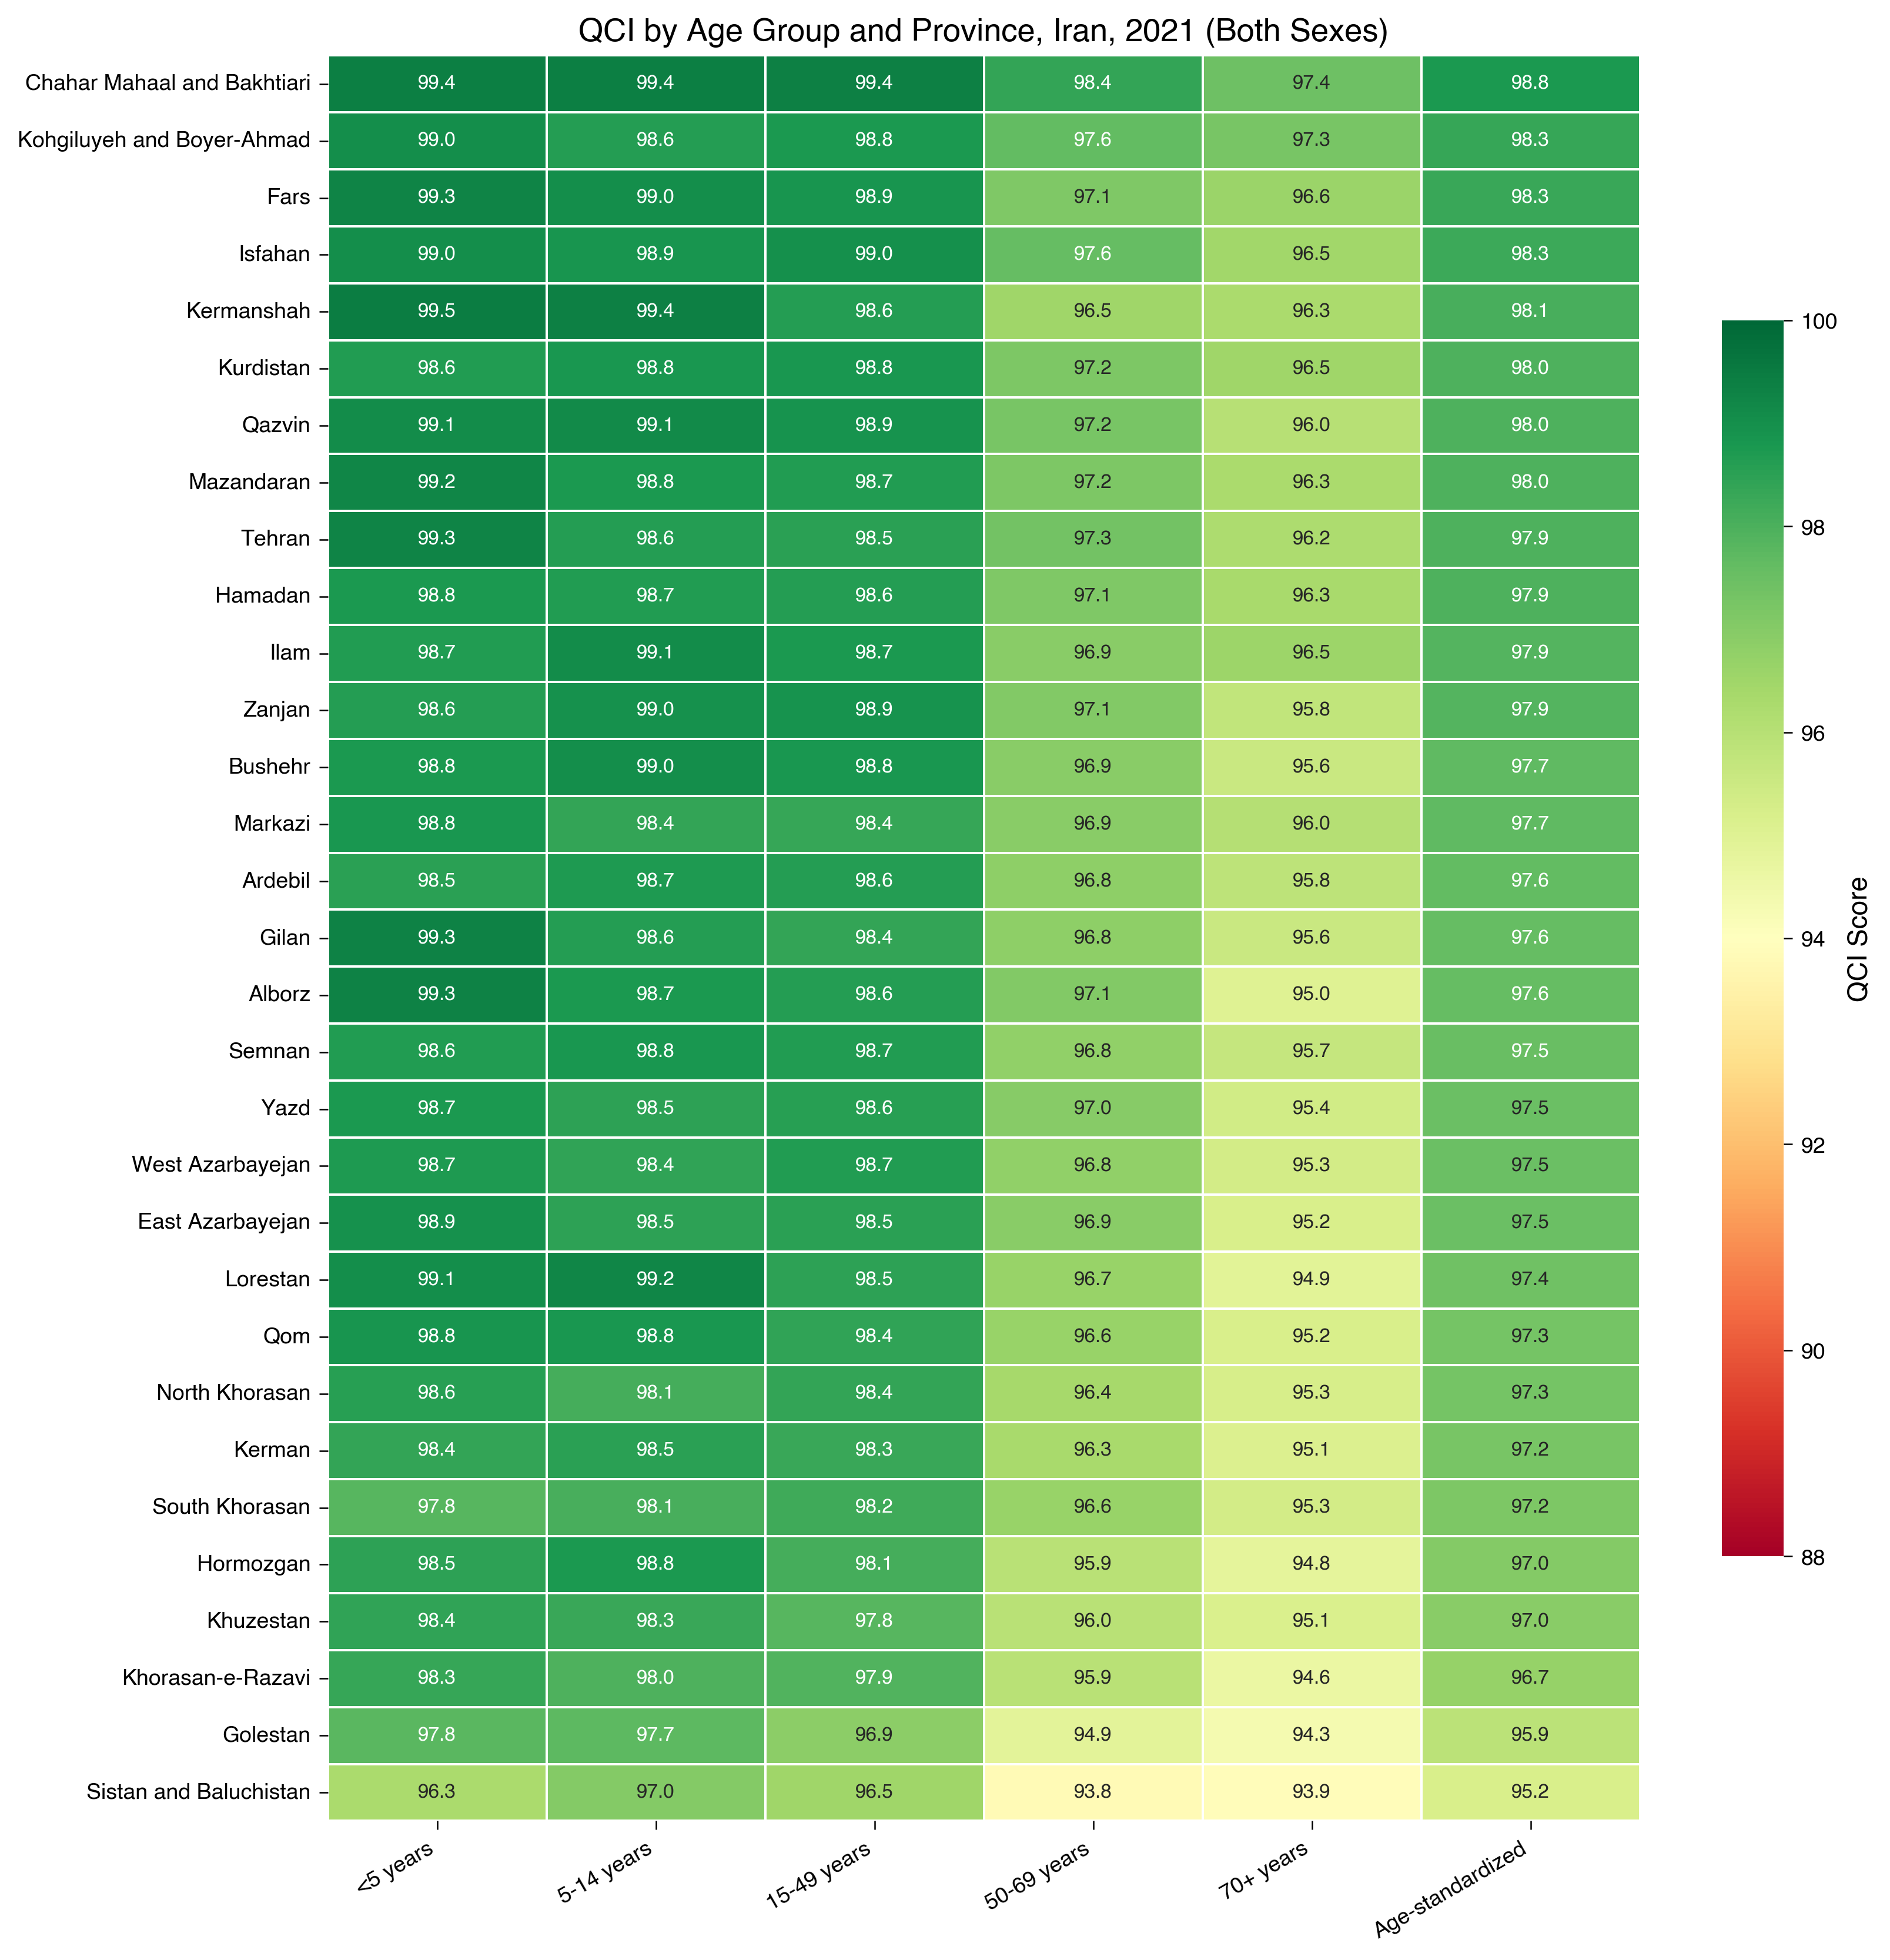
\includegraphics[width=\textwidth]{figure6_age_province_heatmap.png}
\caption{Heatmap of QCI by age group and province, Iran, 2021, both sexes. Children under 5 years show the widest inter-provincial variation and lowest QCI values. Sistan and Baluchistan is the lowest-performing province across all age groups.}
\label{fig:figure6}
\end{figure}

\clearpage

\begin{figure}[htbp]
\centering
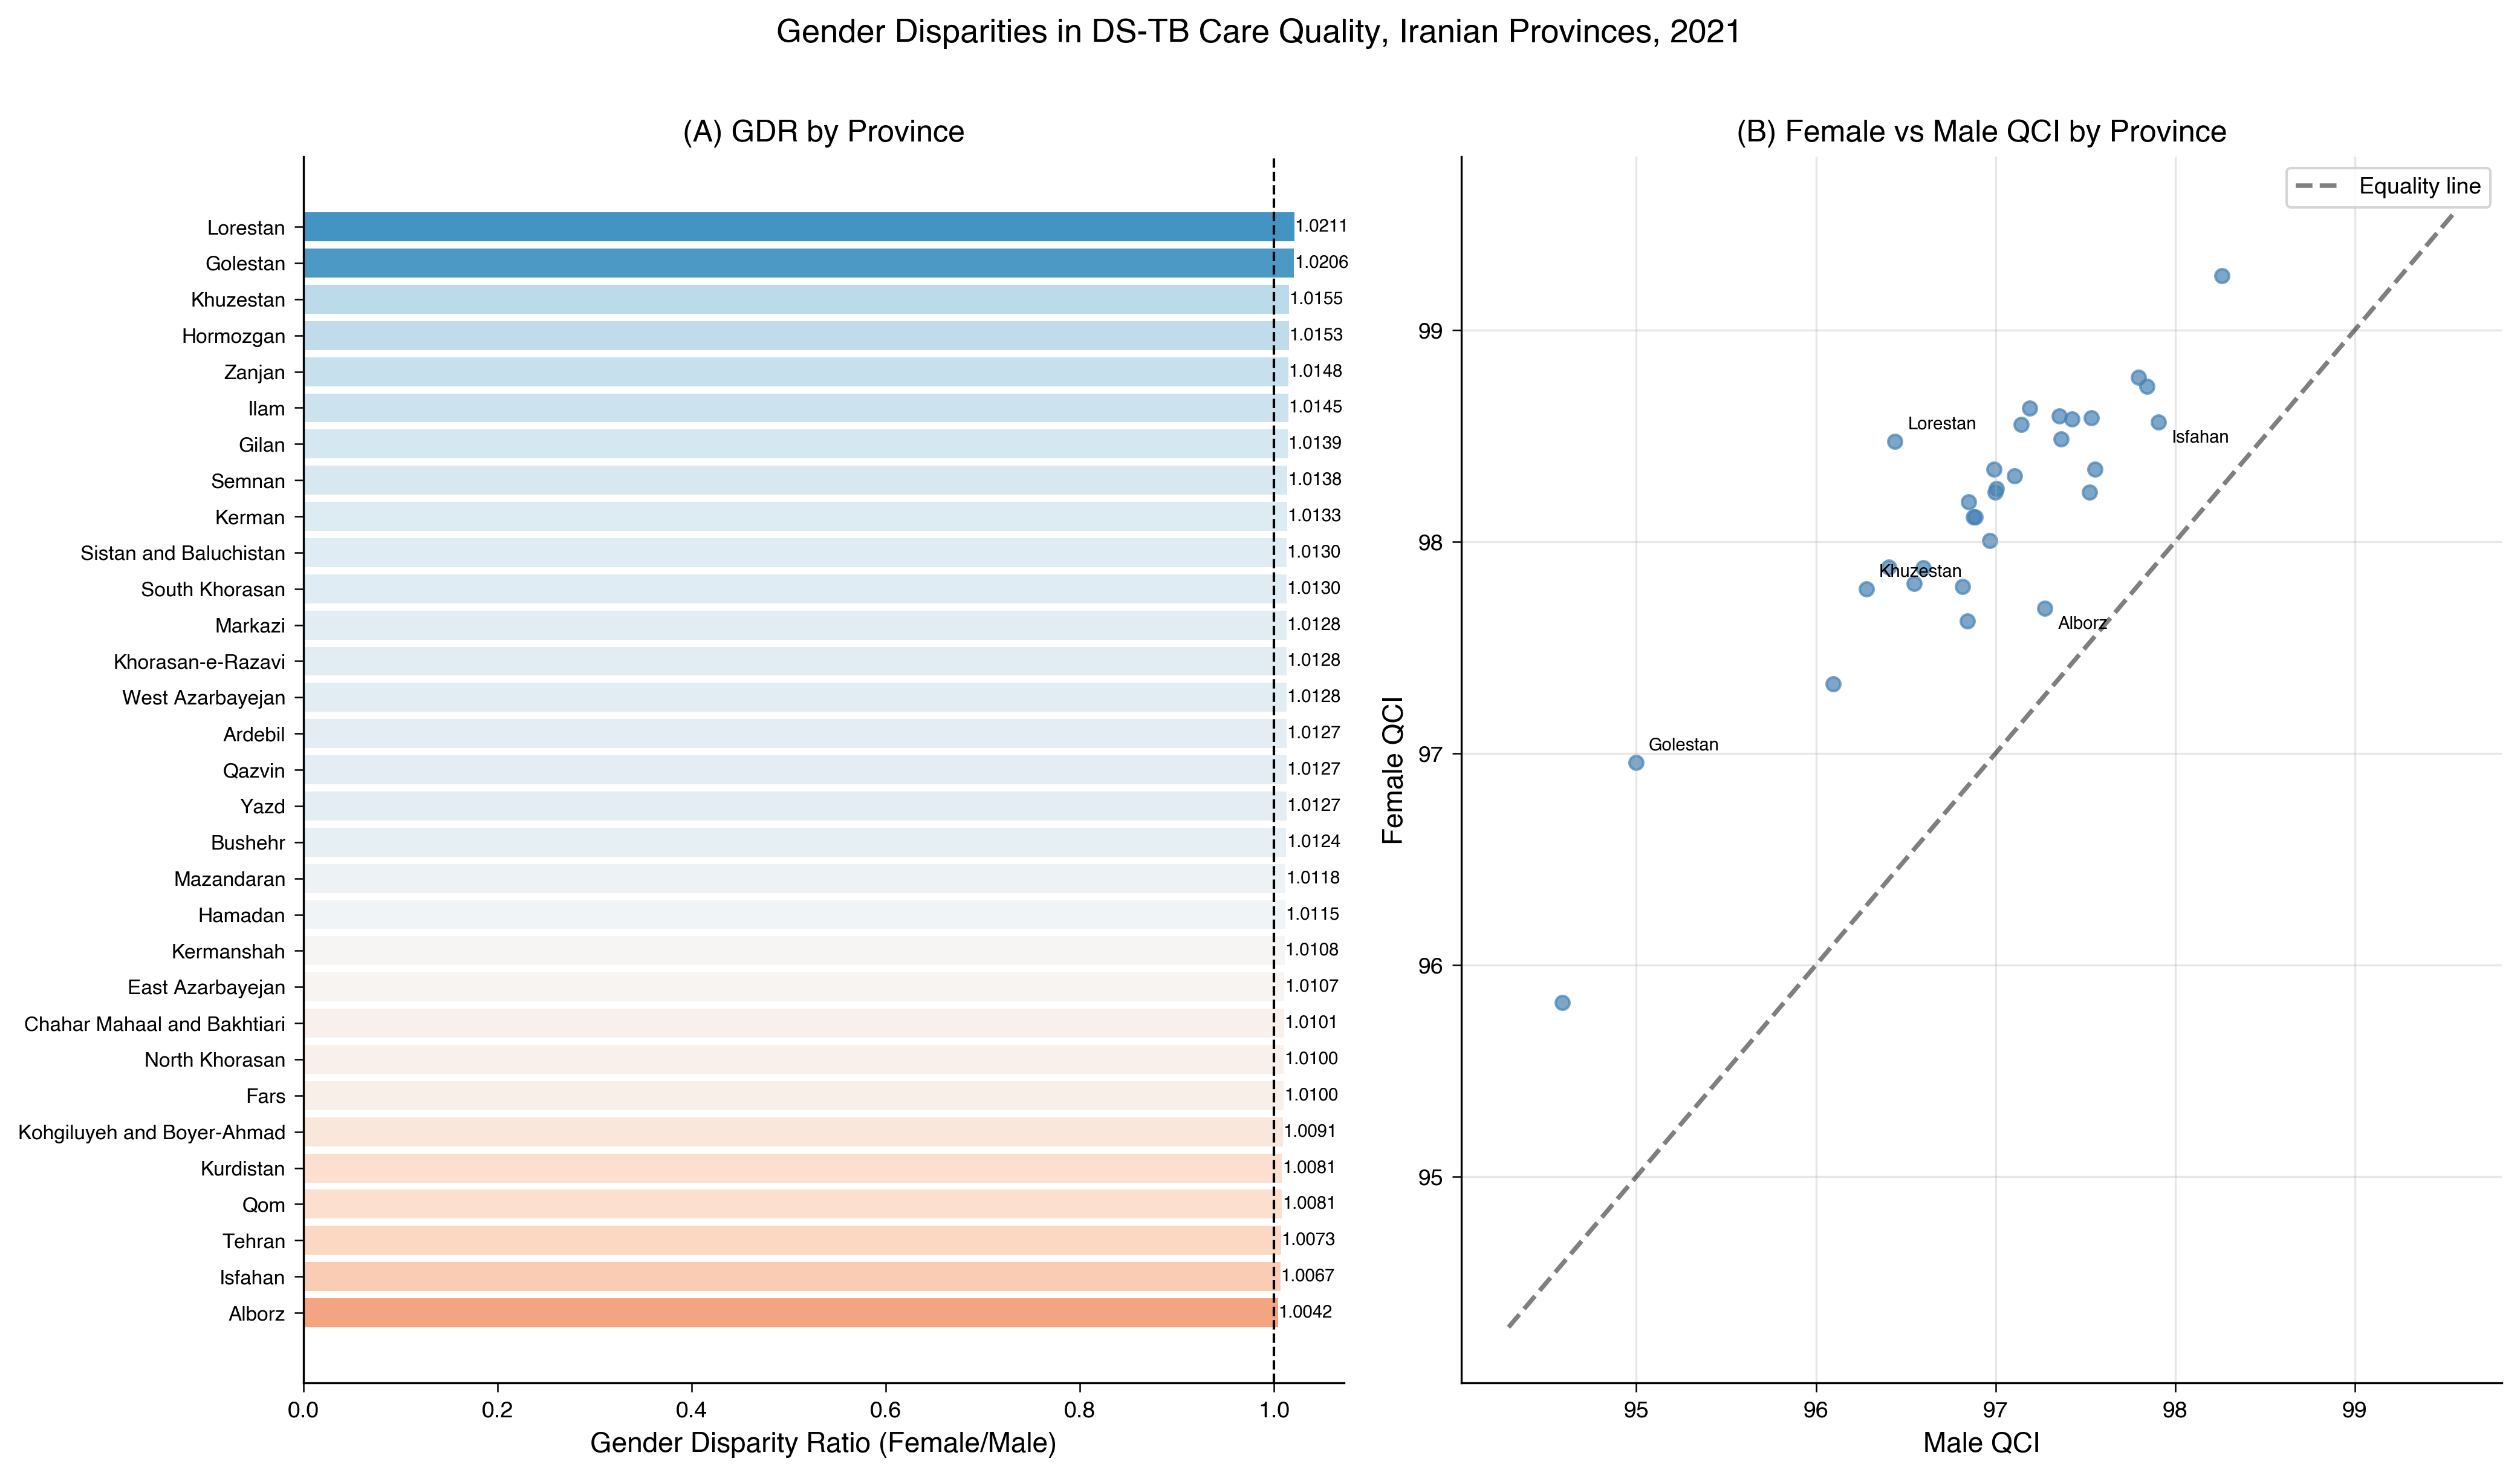
\includegraphics[width=\textwidth]{figure7_gender_disparity.png}
\caption{Gender disparities: (A) GDR by province; (B) female versus male QCI scatter plot. All provinces lie above the equality line, indicating a universal female advantage. The gender gap is widest in less-developed provinces.}
\label{fig:figure7}
\end{figure}

\clearpage

\begin{figure}[htbp]
\centering
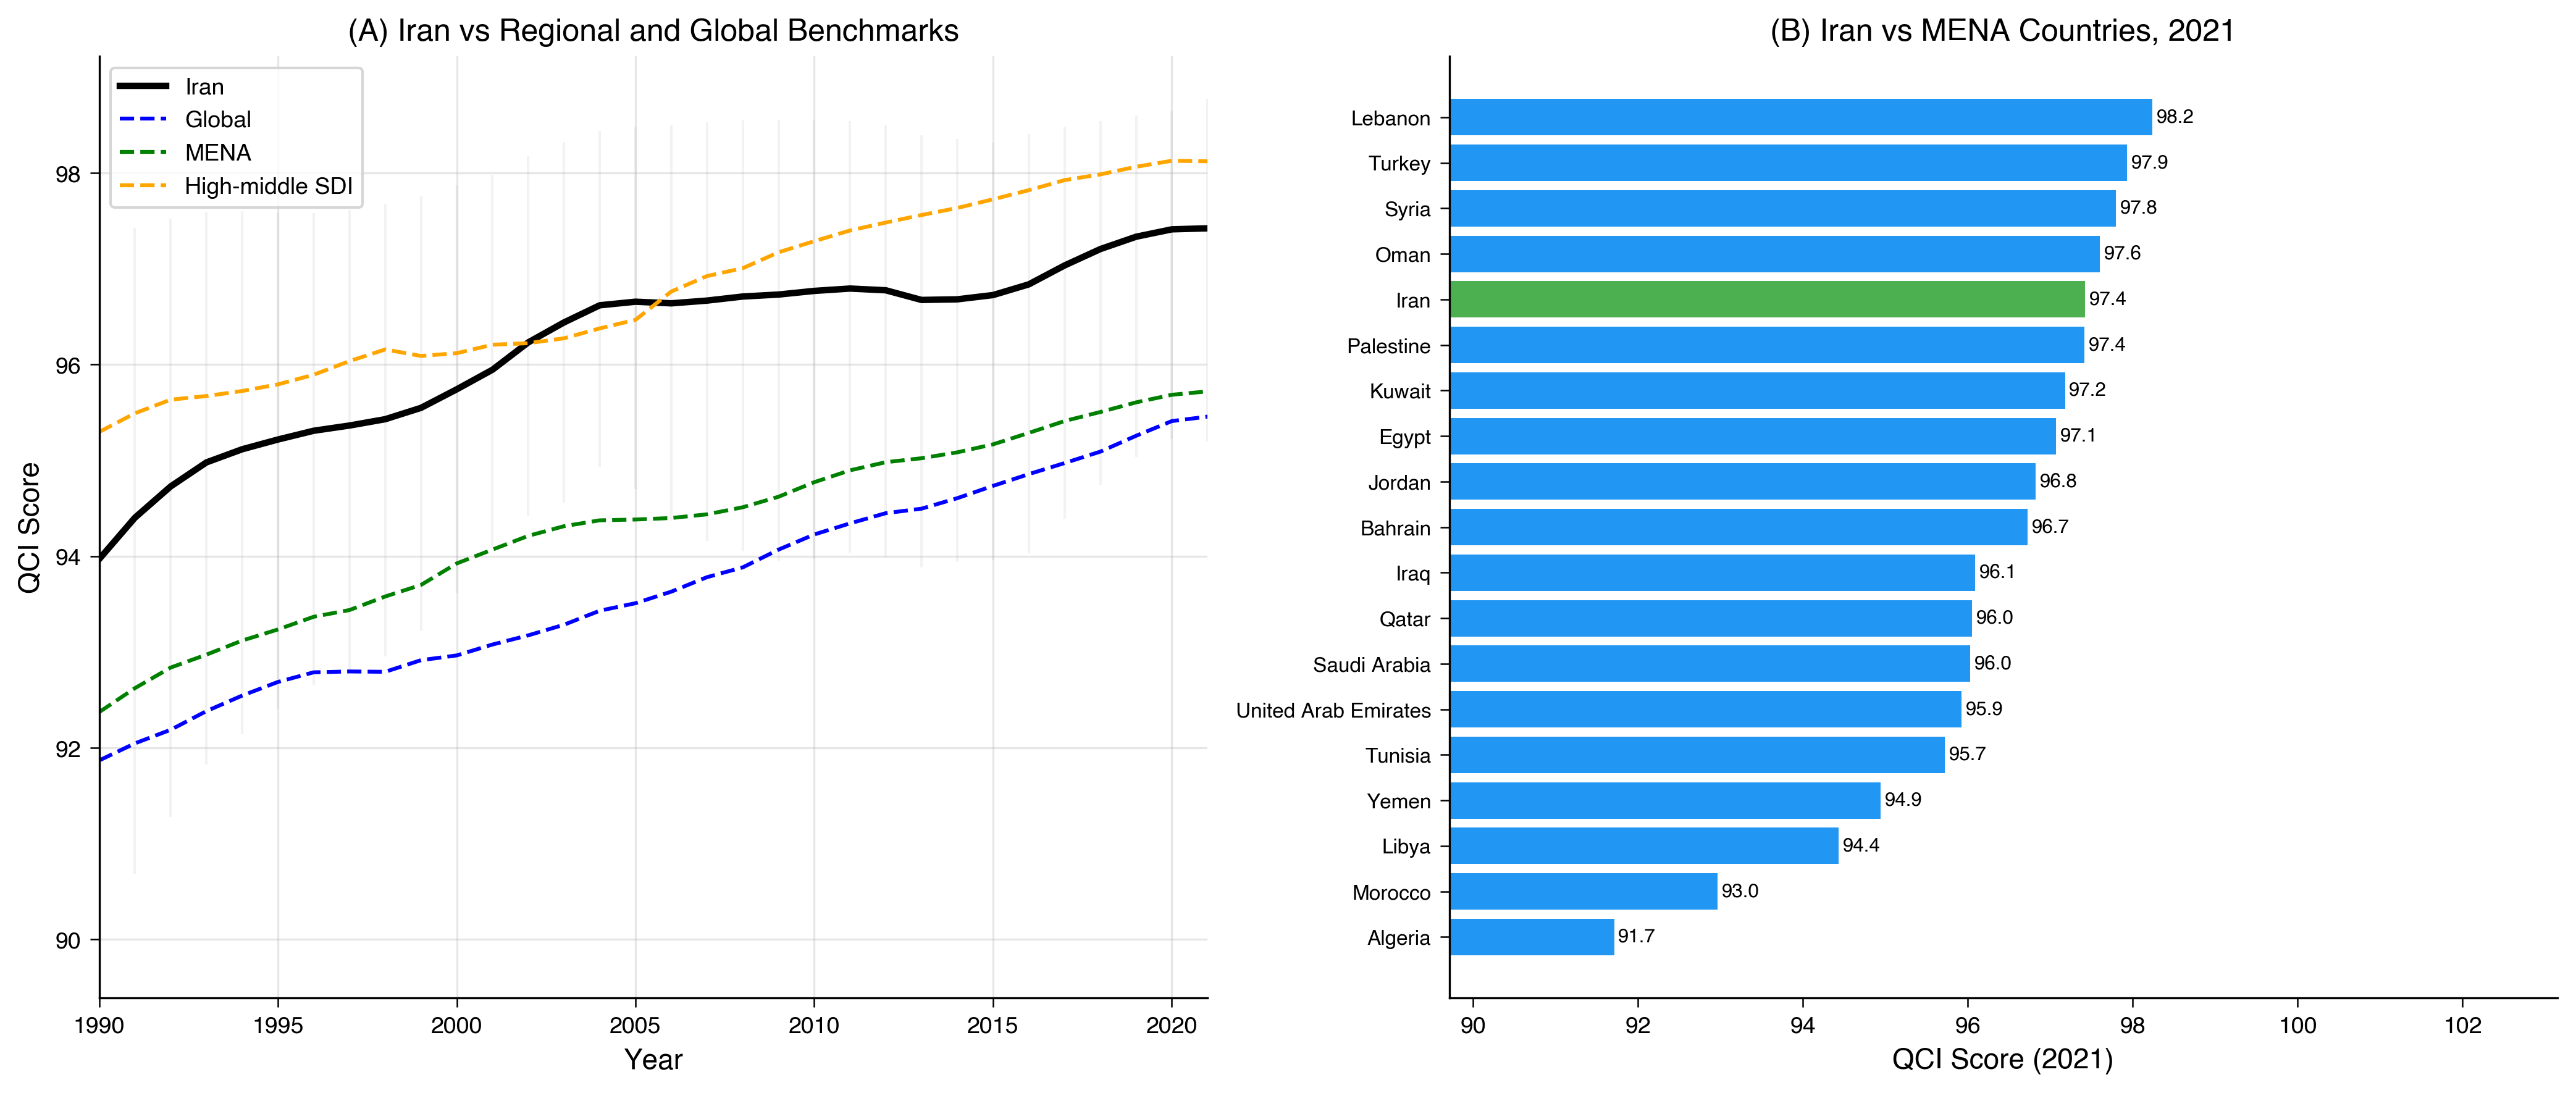
\includegraphics[width=\textwidth]{figure8_iran_vs_benchmarks.png}
\caption{Iran versus regional benchmarks: (A) QCI time series for Iran, Global, MENA, and High-middle SDI, with the grey band showing the provincial range; (B) Iran's rank among MENA countries in 2021.}
\label{fig:figure8}
\end{figure}

\clearpage

\begin{figure}[htbp]
\centering
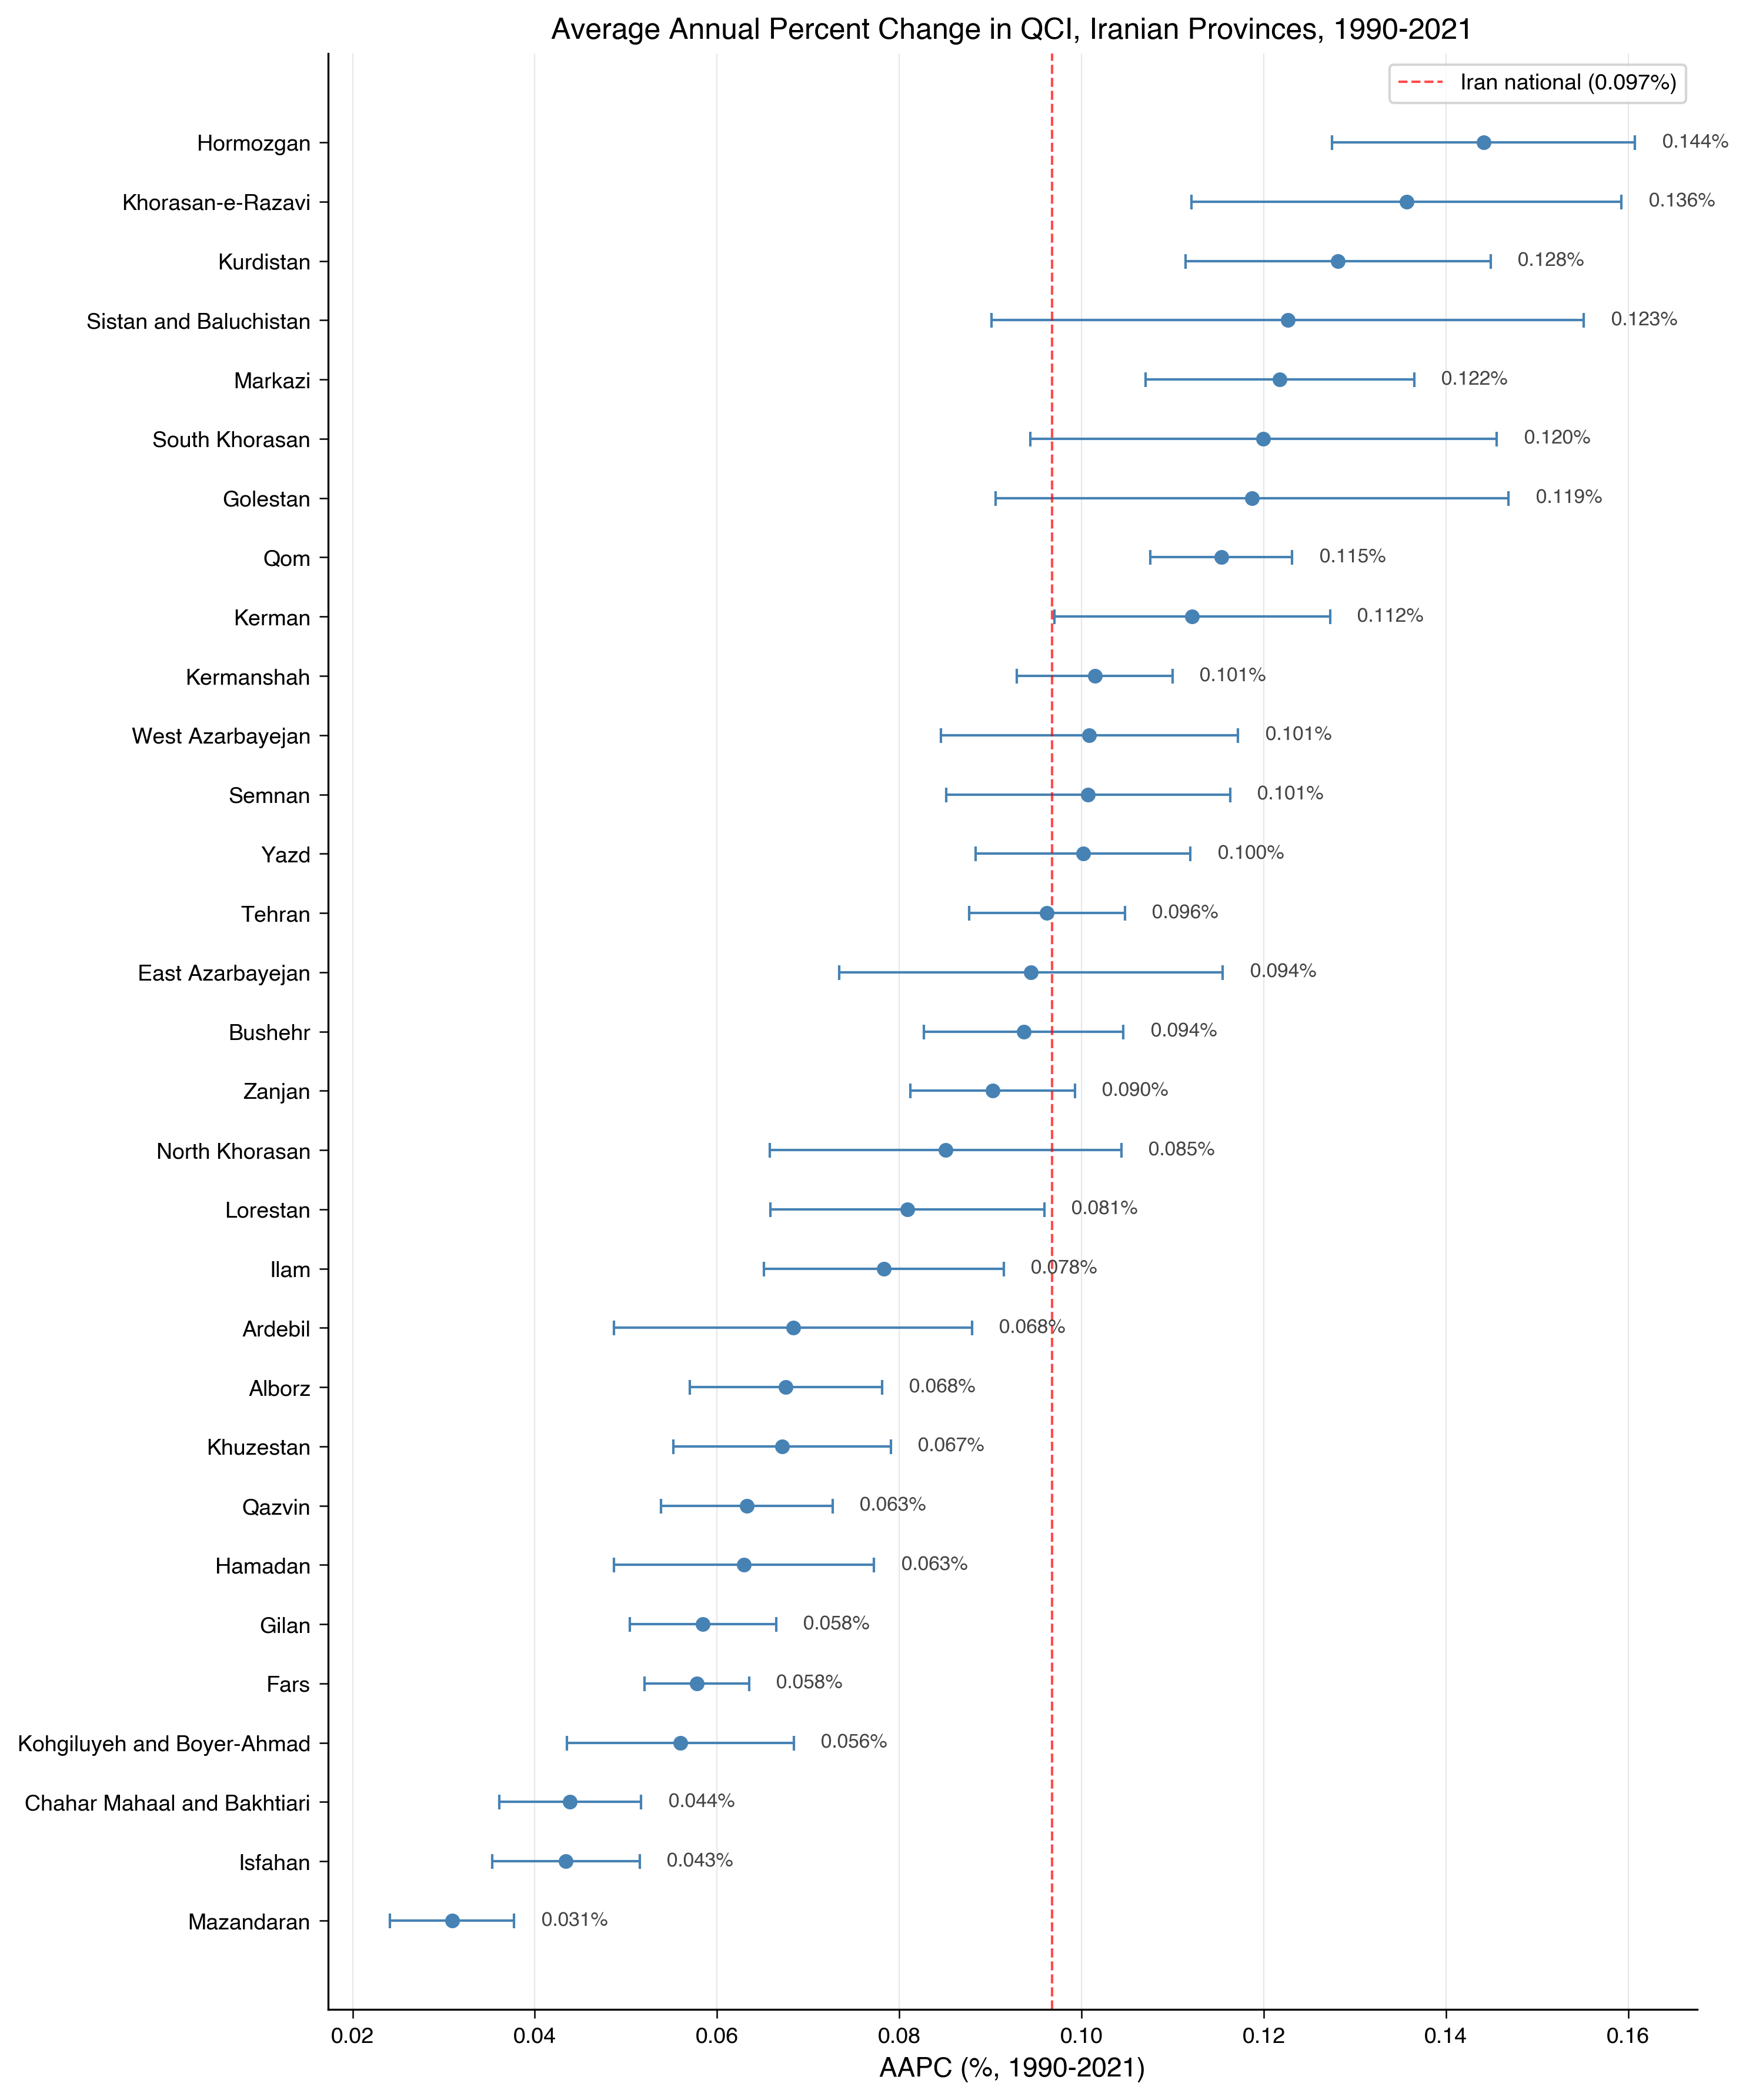
\includegraphics[width=\textwidth]{figure9_aapc_forest_plot.png}
\caption{Forest plot of provincial AAPC in QCI (1990--2021) with 95\% confidence intervals. Red dashed line indicates the national AAPC. Hormozgan and Khorasan-e-Razavi show the fastest improvement rates.}
\label{fig:figure9}
\end{figure}

\clearpage

\begin{figure}[htbp]
\centering
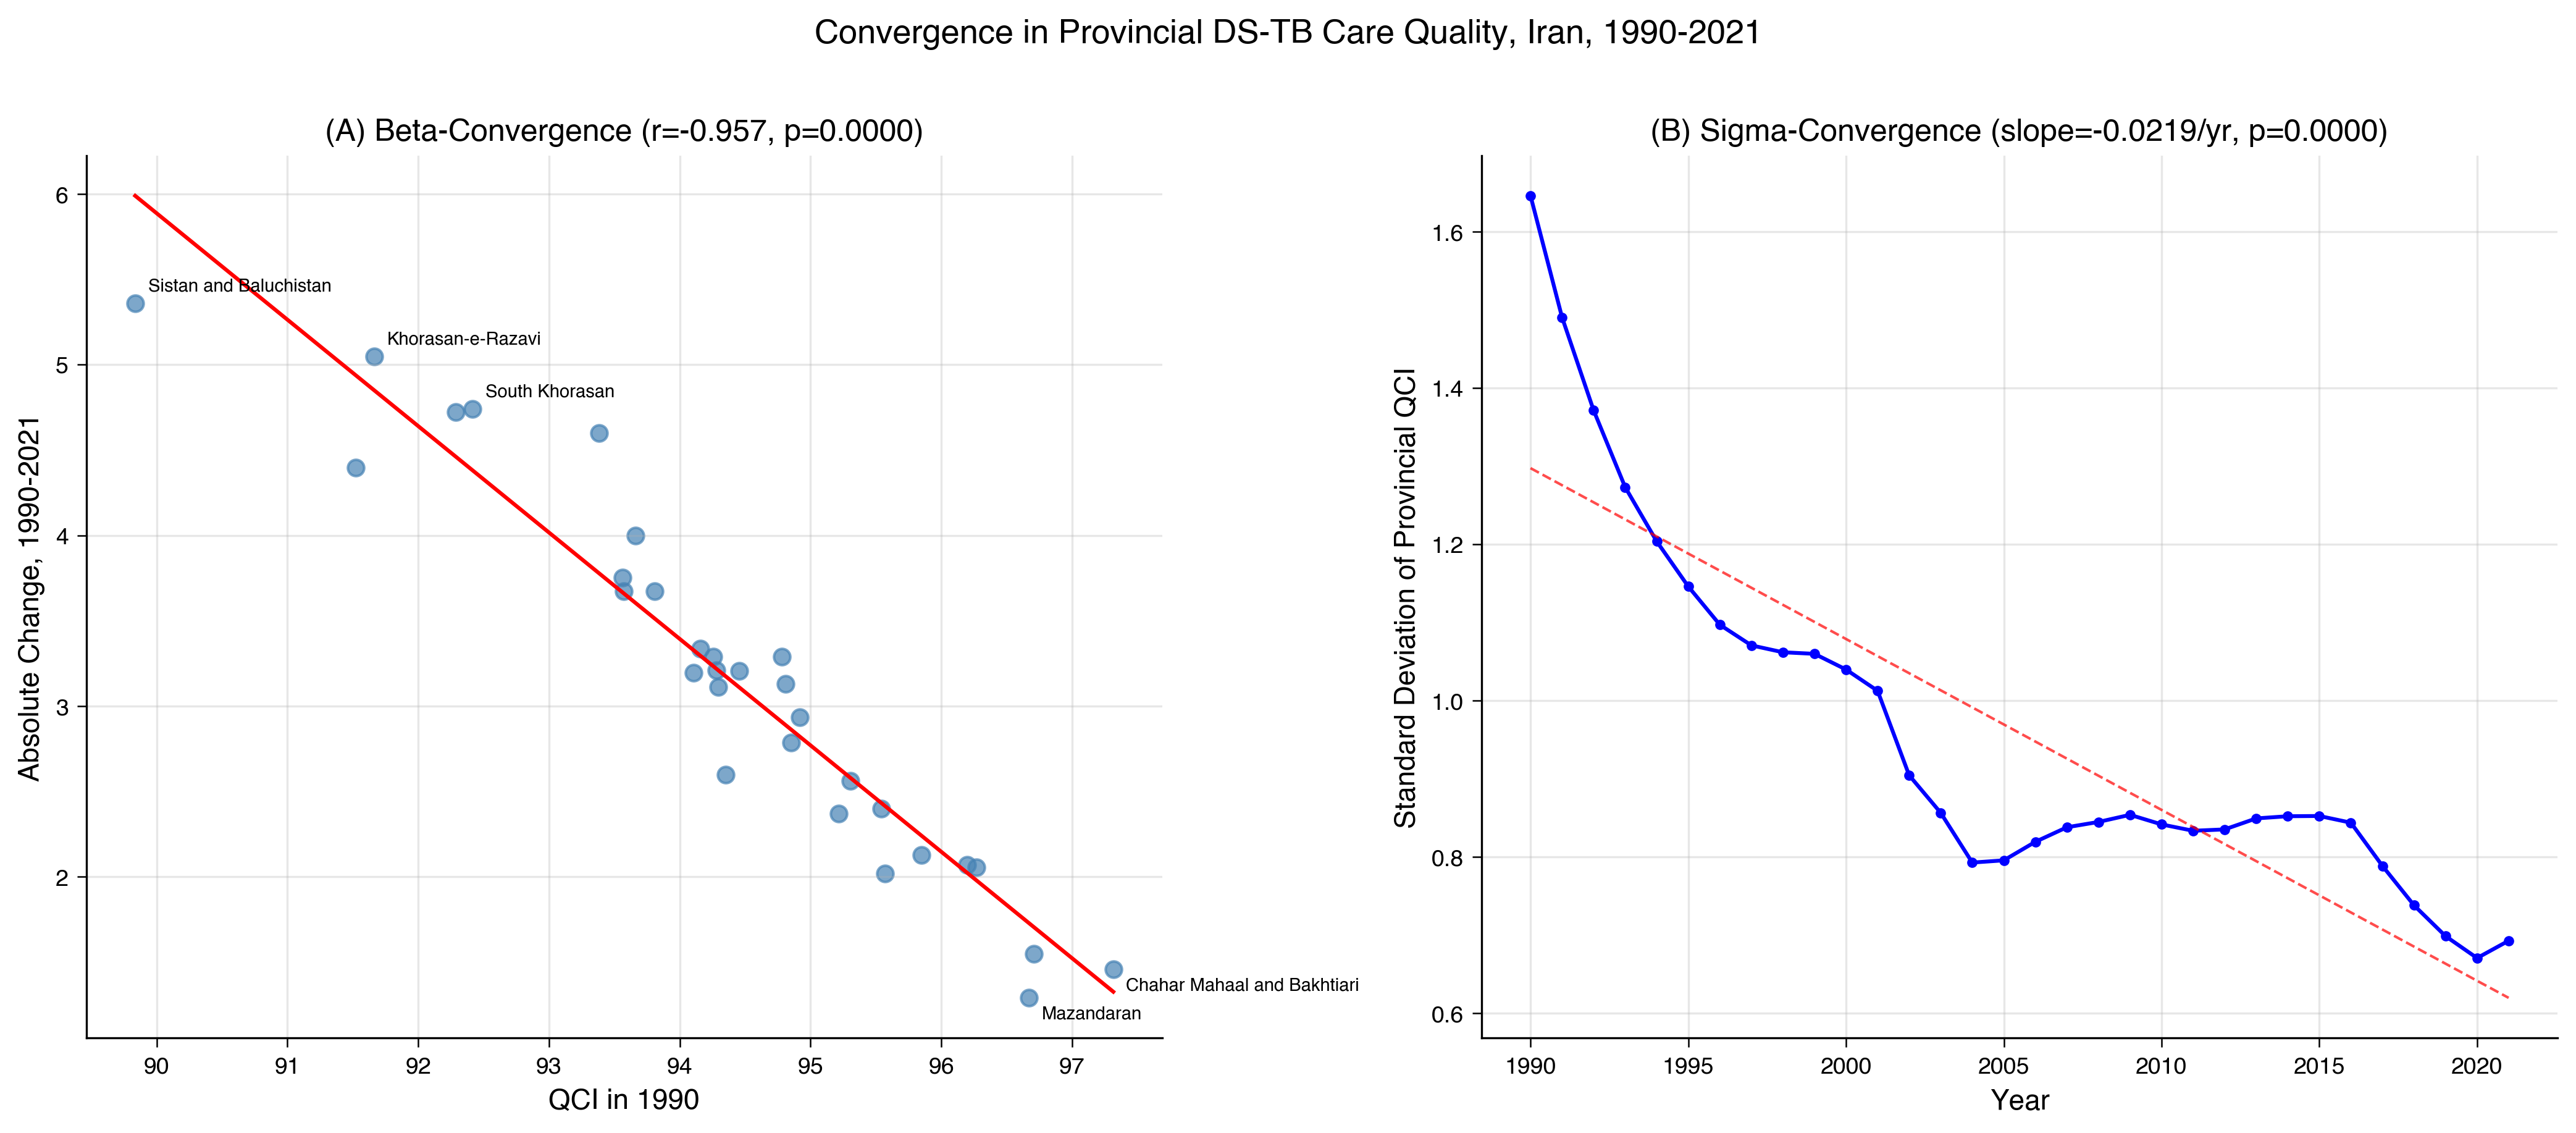
\includegraphics[width=\textwidth]{figure10_convergence.png}
\caption{Convergence analysis: (A) beta-convergence --- provinces with lower 1990 QCI showed larger absolute improvements ($r = -0.958$, $p < 0.001$); (B) sigma-convergence --- the cross-provincial standard deviation declined over time, with a temporary plateau during 2005--2016.}
\label{fig:figure10}
\end{figure}

\clearpage

\begin{figure}[htbp]
\centering
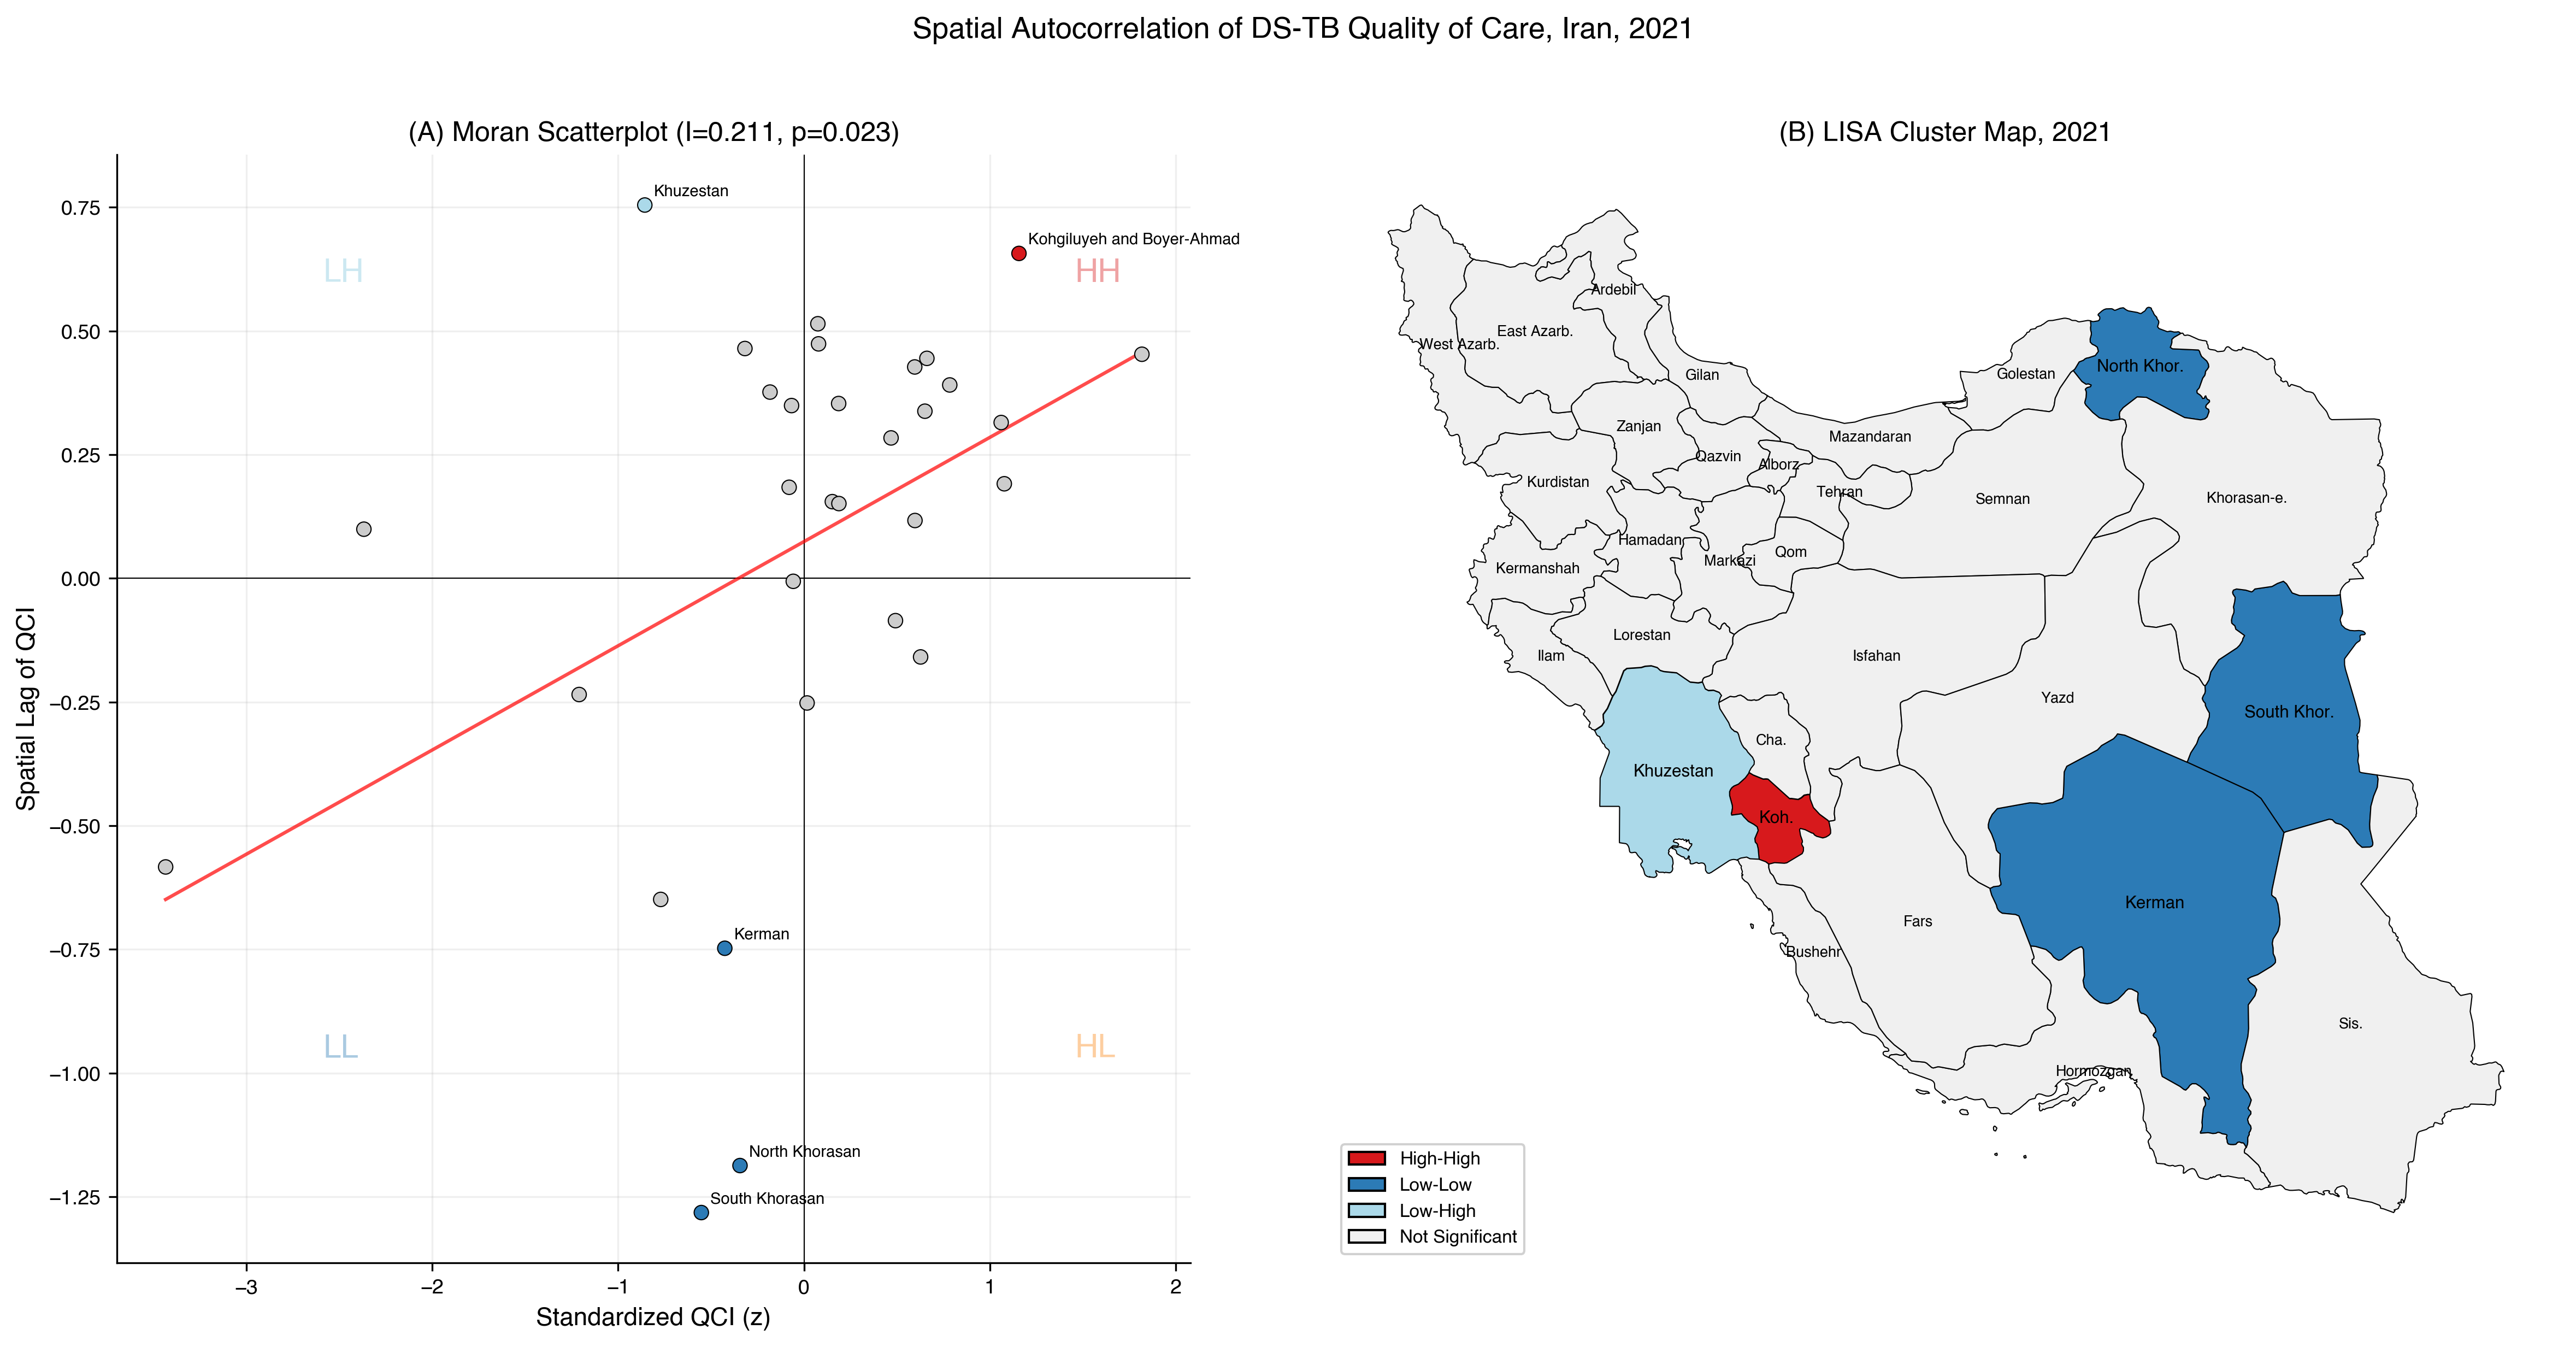
\includegraphics[width=\textwidth]{figure11_lisa_clusters.png}
\caption{Spatial autocorrelation analysis, 2021: (A) Moran scatterplot showing the relationship between standardised QCI and its spatial lag, with significant clusters coloured (HH = red, LL = blue, LH = light blue); (B) LISA cluster map identifying statistically significant spatial clusters --- High-High (Kohgiluyeh and Boyer-Ahmad), Low-Low (North and South Khorasan), and Low-High (Khuzestan).}
\label{fig:figure11}
\end{figure}

\clearpage

\begin{figure}[htbp]
\centering
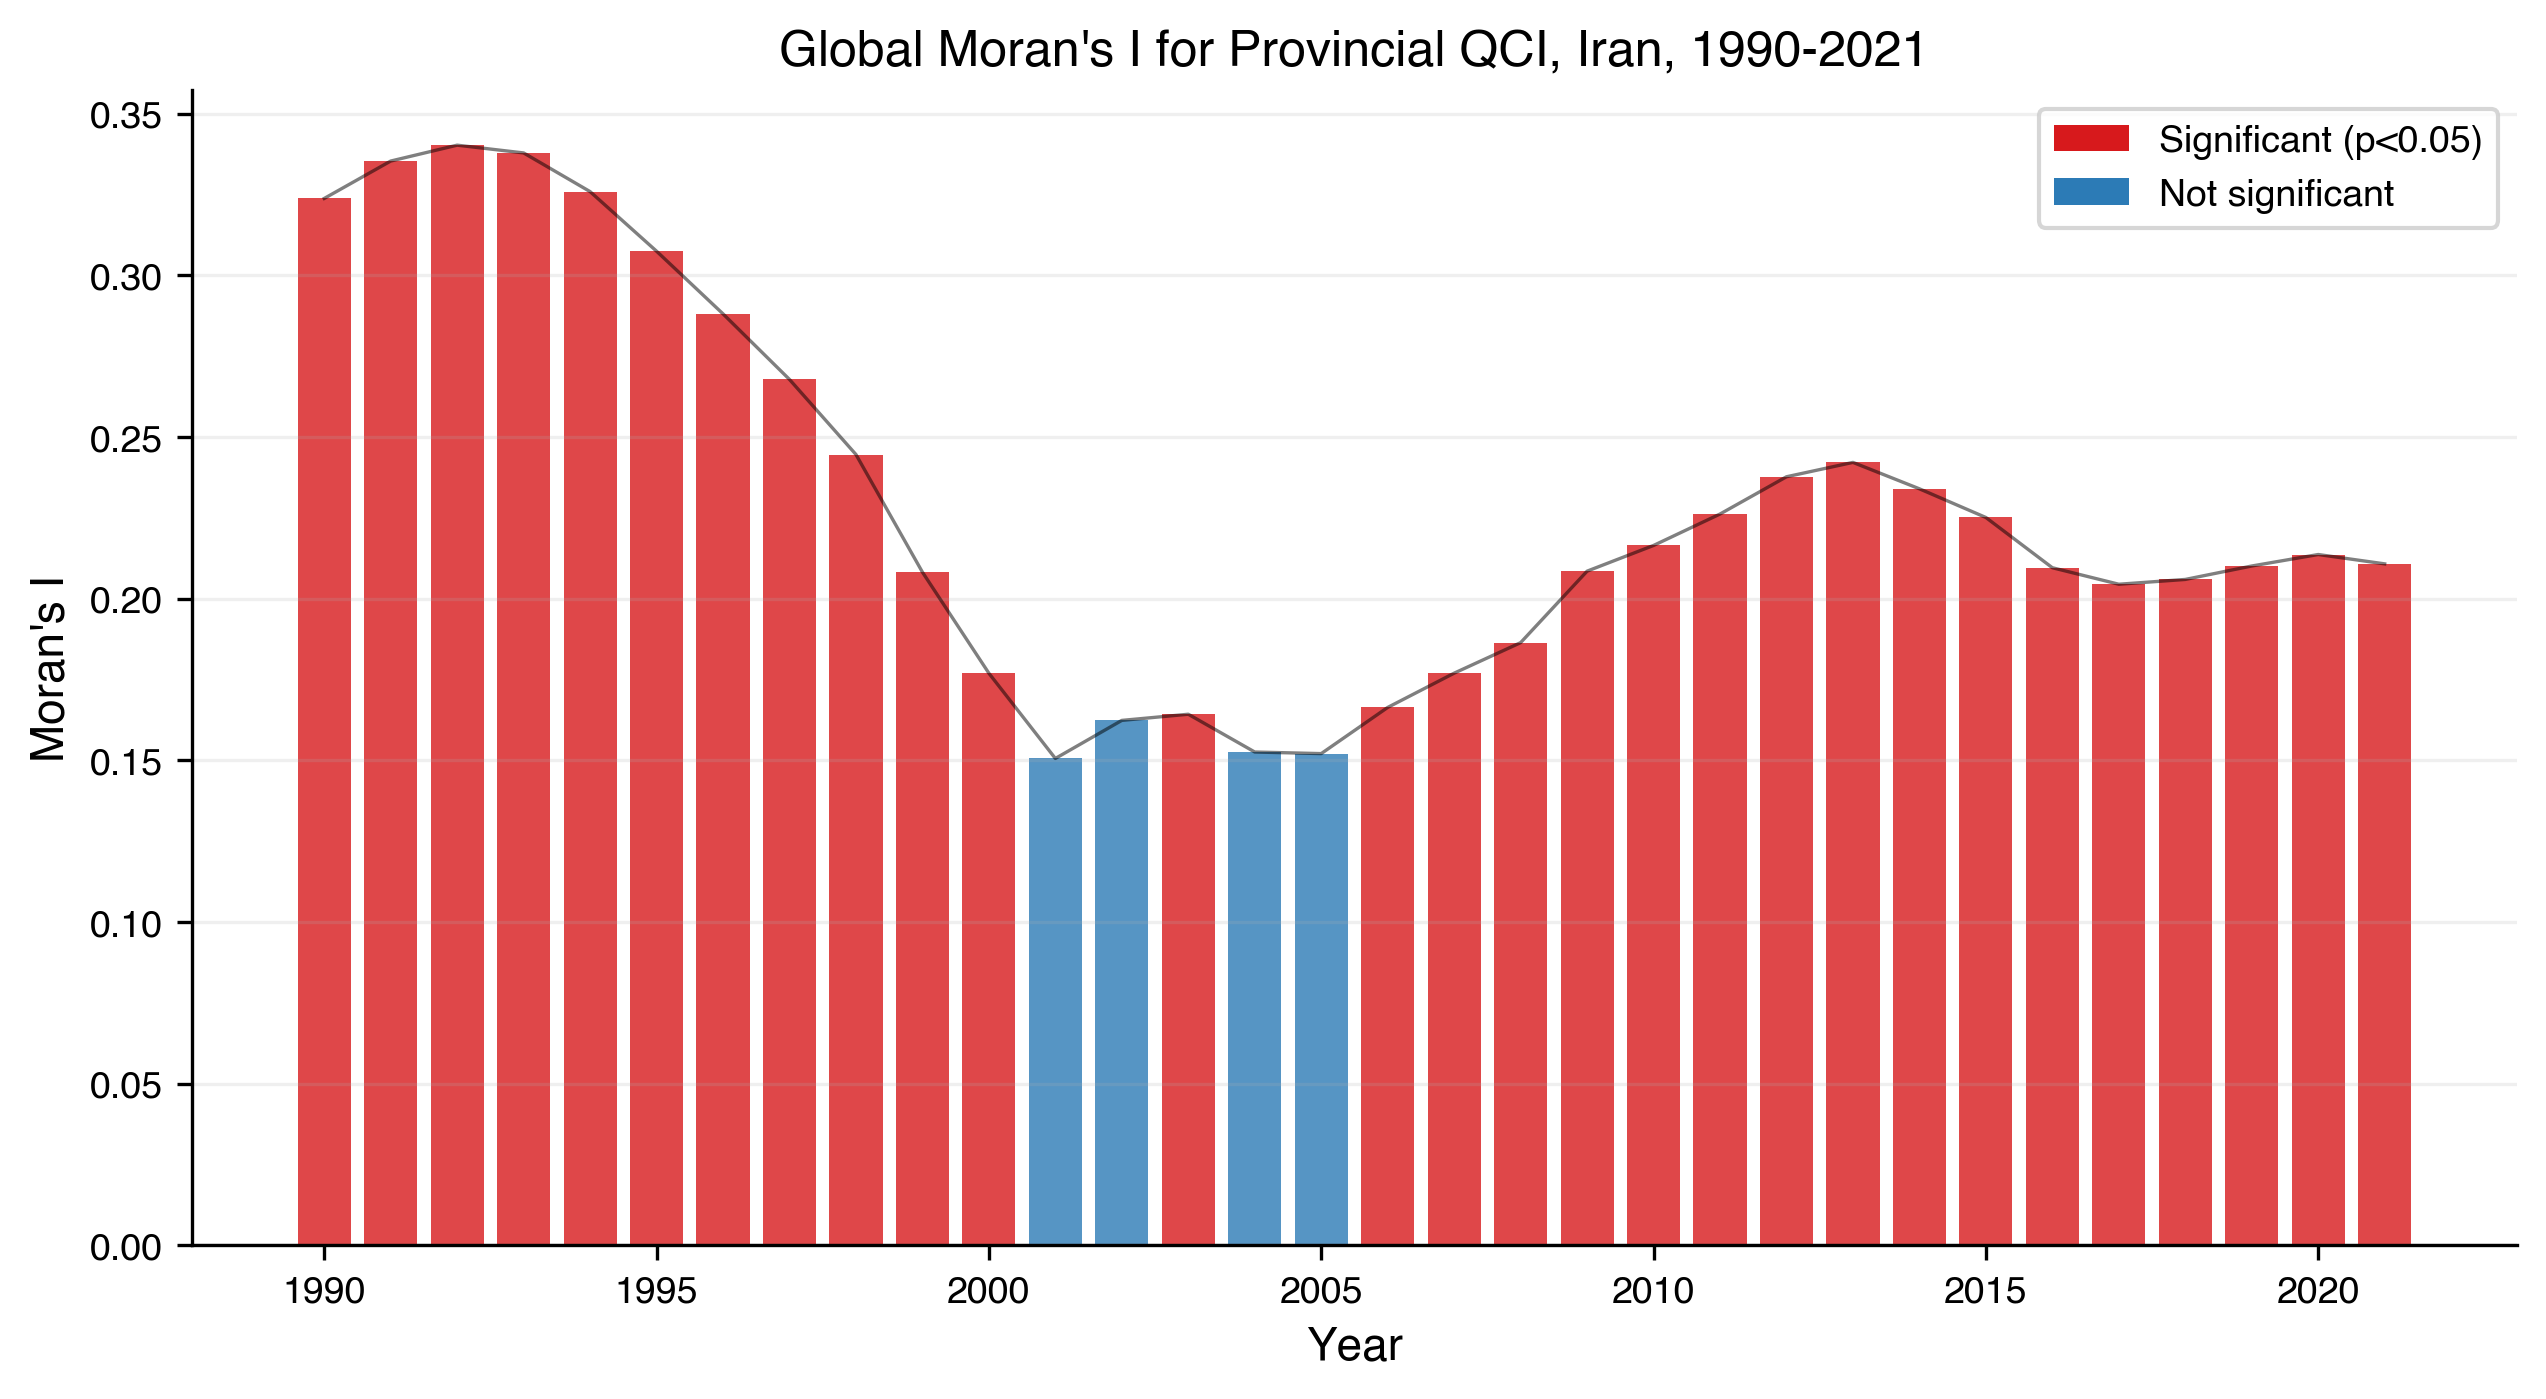
\includegraphics[width=\textwidth]{figure12_morans_i_timeseries.png}
\caption{Global Moran's I for provincial QCI, Iran, 1990--2021. Red bars indicate years with significant spatial autocorrelation ($p < 0.05$). Moran's I was highest in 1990 ($I = 0.324$) and declined over the study period, indicating weakening spatial clustering concurrent with convergence.}
\label{fig:figure12}
\end{figure}

\clearpage

\begin{figure}[htbp]
\centering
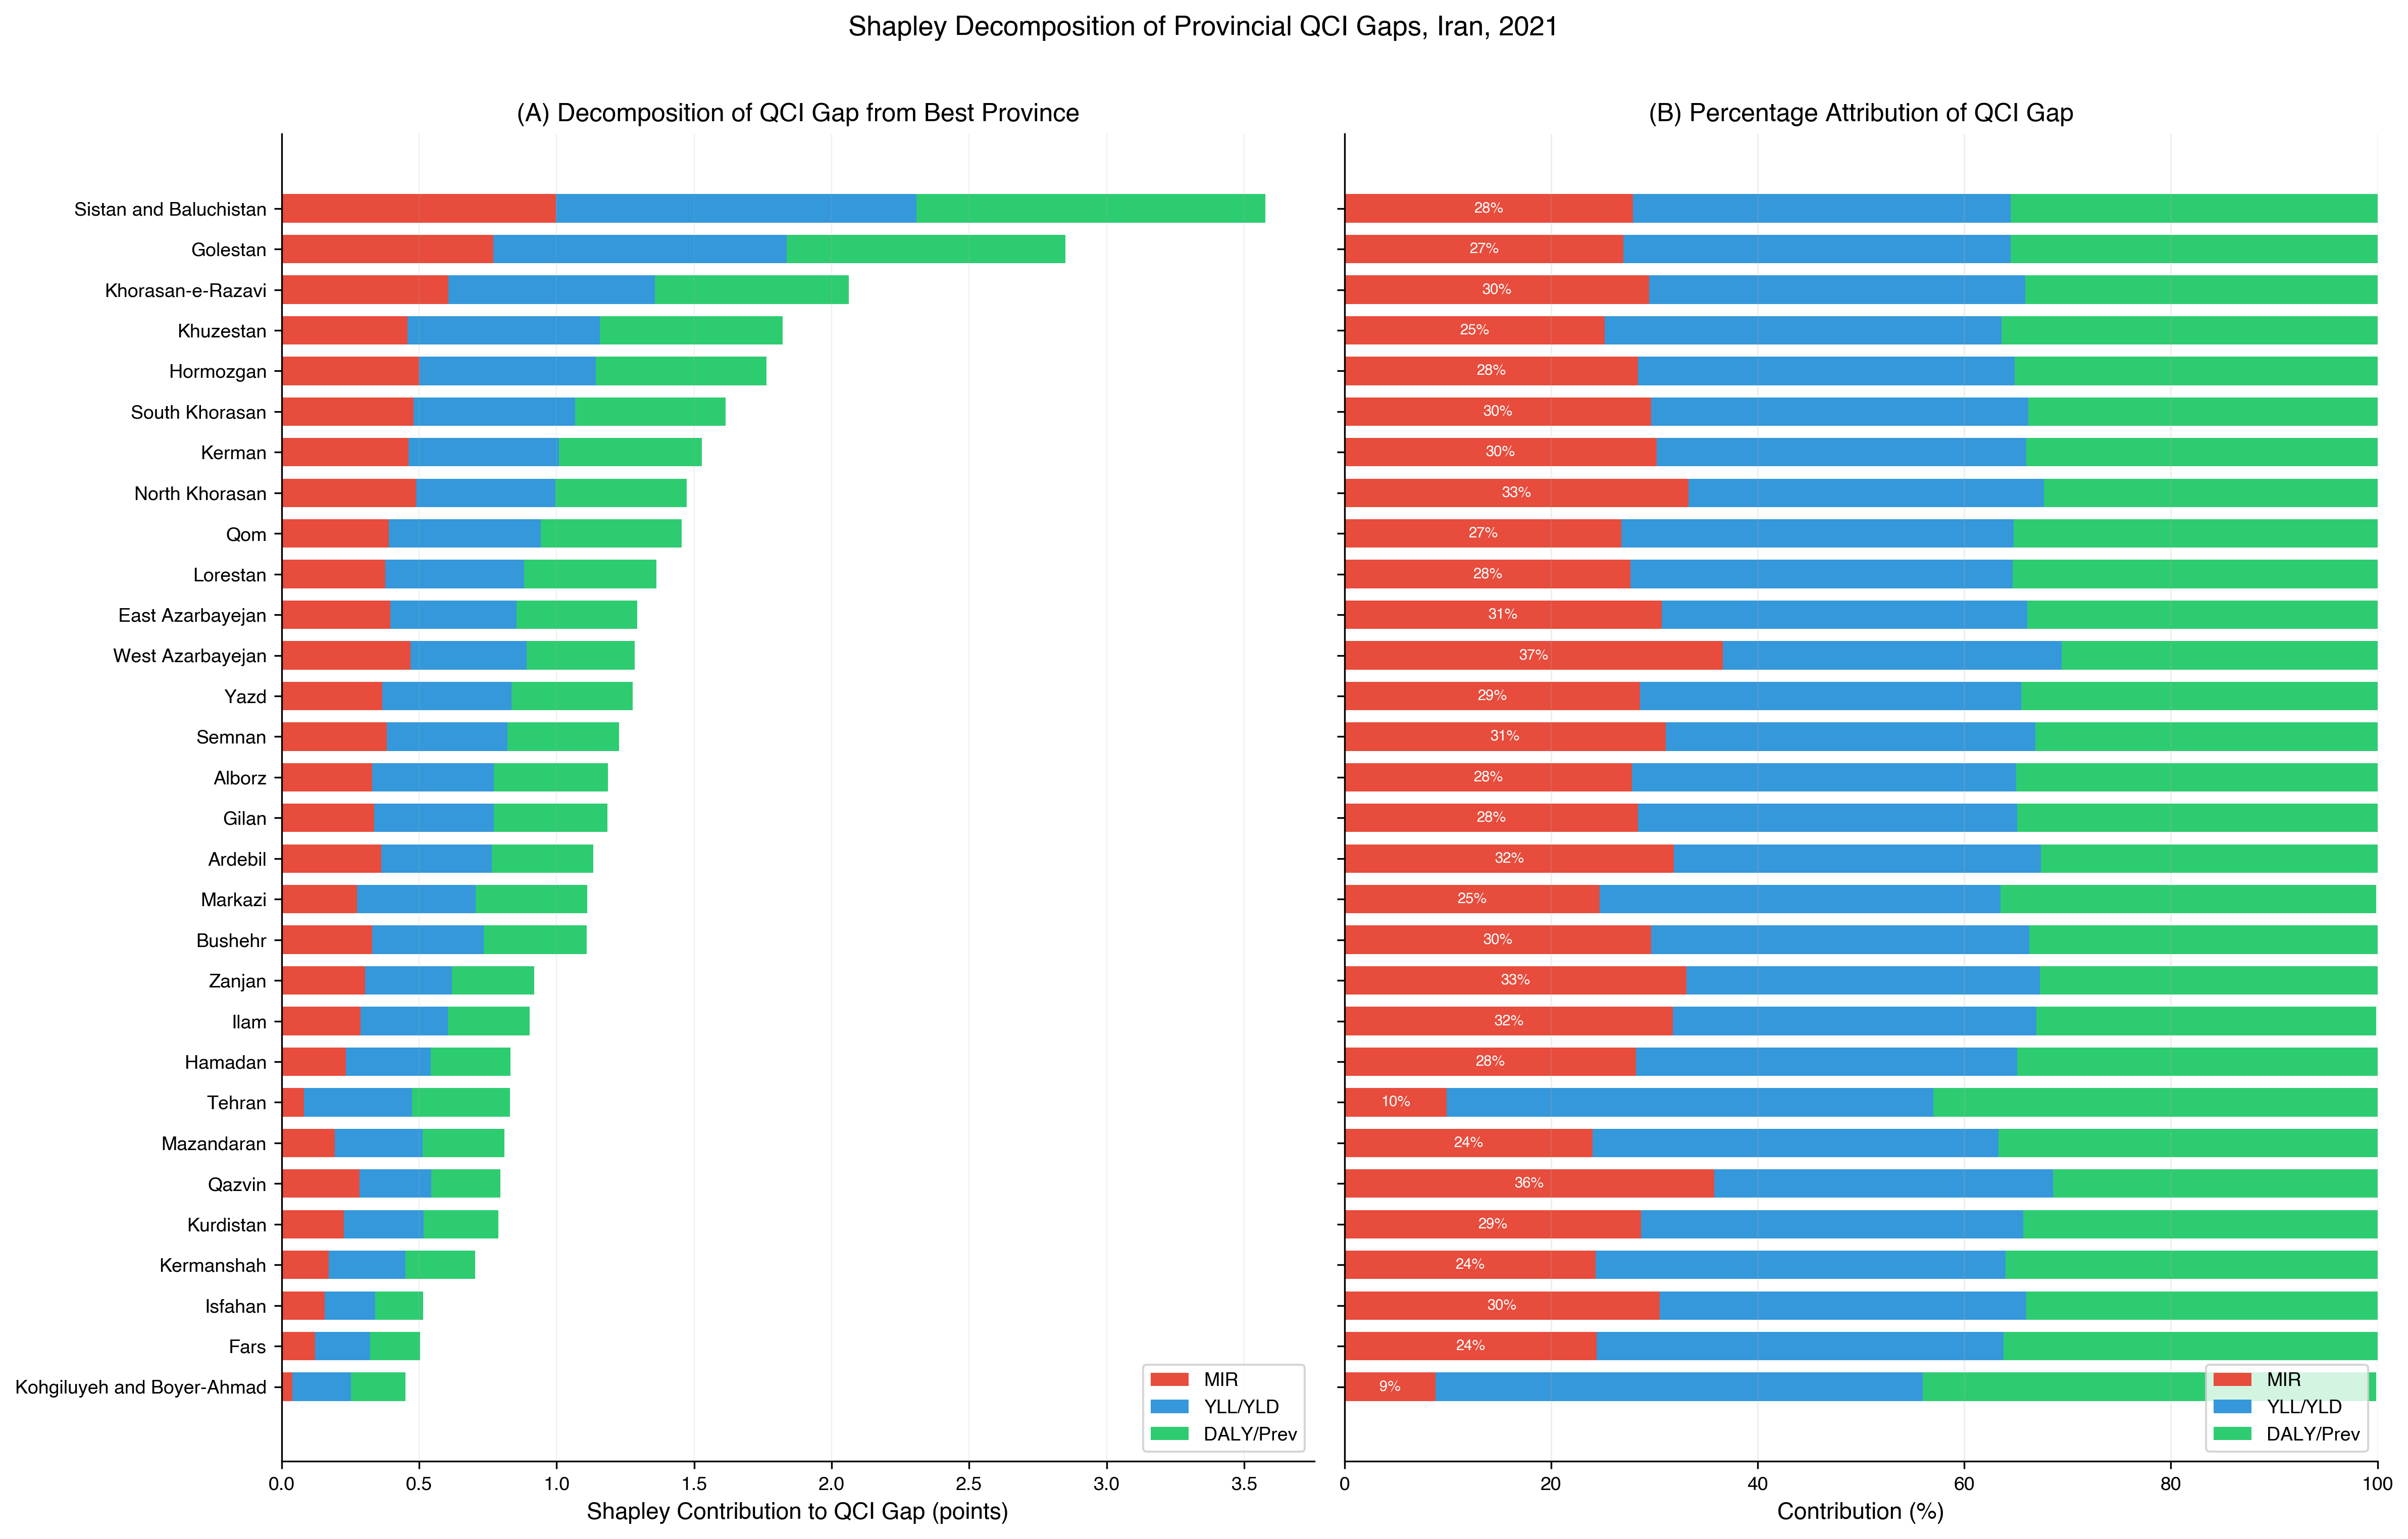
\includegraphics[width=\textwidth]{figure13_shapley_decomposition.png}
\caption{Shapley decomposition of provincial QCI gaps from the best-performing province (Chahar Mahaal and Bakhtiari), 2021: (A) absolute Shapley contributions (points) of MIR, YLL/YLD, and DALY/Prevalence; (B) percentage attribution. The YLL/YLD ratio contributes the largest share of the gap on average (37.2\%), followed by DALY/Prevalence (34.9\%) and MIR (27.8\%).}
\label{fig:figure13}
\end{figure}

%% ============================================================
%% REFERENCES
%% ============================================================

\clearpage

\begin{thebibliography}{31}

\bibitem{ref1}
World Health Organization. Global tuberculosis report 2023. Geneva: WHO; 2023.

\bibitem{ref2}
Global Burden of Disease Collaborative Network. Global Burden of Disease Study 2021 (GBD 2021) Results. Seattle, United States: Institute for Health Metrics and Evaluation (IHME), 2022. Available from \url{https://vizhub.healthdata.org/gbd-results/}.

\bibitem{ref3}
Nasehi M, Mirhaghani L. National guideline for tuberculosis control. Tehran: Ministry of Health and Medical Education; 2019.

\bibitem{ref4}
Haghdoost AA, Rezazadeh-Kermani M, Sadghirad B, Baradaran HR. Epidemiology of tuberculosis in Iran. \textit{Eastern Mediterranean Health Journal} 2009; \textbf{15}: 235--41.

\bibitem{ref5}
[Authors]. Global, Regional, and National Quality of Care Index for Drug-Susceptible Tuberculosis, 1990--2021: A Systematic Analysis of the Global Burden of Disease Study 2021. [Manuscript submitted for publication].

\bibitem{ref6}
GBD 2019 Healthcare Access and Quality Collaborators. Assessing performance of the Healthcare Access and Quality Index for 204 countries and territories, 1990--2019. \textit{Lancet Glob Health} 2022; \textbf{10}: e1715--43.

\bibitem{ref7}
World Health Organization. The End TB Strategy. Geneva: WHO; 2015.

\bibitem{ref8}
Moradi-Lakeh M, Vosoogh-Moghaddam A. Health sector evolution plan in Iran; equity and sustainability concerns. \textit{Int J Health Policy Manag} 2015; \textbf{4}: 637--40.

\bibitem{ref9}
Rashidian A, Khosravi A, Khabiri R, et al. Islamic Republic of Iran's Health System Challenges, Achievements, and Lessons Learned. \textit{East Mediterr Health J} 2019; \textbf{25}: 835--43.

\bibitem{ref10}
Sharifi H, Mirzazadeh A, Noroozi A, et al. Estimating the prevalence of tuberculosis in Sistan and Baluchistan province, Iran: a capture-recapture study. \textit{Int J Tuberc Lung Dis} 2020; \textbf{24}: 1239--44.

\bibitem{ref11}
Horton KC, MacPherson P, Houben RMGJ, et al. Sex differences in tuberculosis burden and notifications in low- and middle-income countries: a systematic review and meta-analysis. \textit{PLoS Med} 2016; \textbf{13}: e1002119.

\bibitem{ref12}
Dodd PJ, Yuen CM, Sismanidis C, et al. The global burden of tuberculosis mortality in children: a mathematical modelling study. \textit{Lancet Glob Health} 2017; \textbf{5}: e898--906.

\bibitem{ref13}
Setayesh S, Mackey TK. Addressing the impact of economic sanctions on Iranian drug shortages in the joint comprehensive plan of action: promoting access to medicines and health diplomacy. \textit{Global Health} 2016; \textbf{12}: 31.

\bibitem{ref14}
Heshmati B, Joulaei H. Iran's health-care system in transition. \textit{Lancet} 2016; \textbf{387}: 29--30.

\bibitem{ref15}
GBD 2021 Diseases and Injuries Collaborators. Global, regional, and national incidence, prevalence, and years lived with disability for 354 diseases and injuries, 1990--2021. \textit{Lancet} 2024; \textbf{403}: 2162--203.

\bibitem{ref16}
GBD 2021 Causes of Death Collaborators. Global, regional, and national age-sex-specific mortality for 288 causes of death, 1990--2021. \textit{Lancet} 2024; \textbf{403}: 2100--32.

\bibitem{ref17}
Kruk ME, Gage AD, Arsenault C, et al. High-quality health systems in the Sustainable Development Goals era: time for a revolution. \textit{Lancet Glob Health} 2018; \textbf{6}: e1196--252.

\bibitem{ref18}
Subbaraman R, Nathavitharana RR, Mayer KH, et al. Constructing care cascades for active tuberculosis: a strategy for program monitoring and identifying gaps in quality of care. \textit{PLoS Med} 2019; \textbf{16}: e1002754.

\bibitem{ref19}
Anselin L. Local Indicators of Spatial Association---LISA. \textit{Geogr Anal} 1995; \textbf{27}: 93--115.

\bibitem{ref20}
Rey SJ, Anselin L. PySAL: A Python Library of Spatial Analytical Methods. \textit{Rev Reg Stud} 2007; \textbf{37}: 5--27.

\bibitem{ref21}
Shorrocks AF. Decomposition procedures for distributional analysis: a unified framework based on the Shapley value. \textit{J Econ Inequal} 2013; \textbf{11}: 99--126.

\bibitem{ref22}
GBD 2016 Healthcare Access and Quality Collaborators. Measuring performance on the Healthcare Access and Quality Index for 195 countries and territories and selected subnational locations: a systematic analysis from the Global Burden of Disease Study 2016. \textit{Lancet} 2018; \textbf{391}: 2236--71.

\bibitem{ref23}
Nhamoyebonde S, Leslie A. Biological differences between the sexes and susceptibility to tuberculosis. \textit{J Infect Dis} 2014; \textbf{209} (suppl 3): S100--6.

\bibitem{ref24}
Pourshams A, Khademi H, Malekshah AF, et al. Cohort profile: the Golestan Cohort Study --- a prospective study of oesophageal cancer in northern Iran. \textit{Int J Epidemiol} 2010; \textbf{39}: 52--59.

\bibitem{ref25}
Zar HJ, Hanslo D, Apolles P, Swingler G, Hussey G. Induced sputum versus gastric lavage for microbiological confirmation of pulmonary tuberculosis in infants and young children: a prospective study. \textit{Lancet} 2005; \textbf{365}: 130--34.

\bibitem{ref26}
World Health Organization. WHO operational handbook on tuberculosis. Module 2: screening --- systematic screening for tuberculosis disease. Geneva: WHO; 2021.

\bibitem{ref27}
World Health Organization. Guidance for national tuberculosis programmes on the management of tuberculosis in children, 2nd edn. Geneva: WHO; 2014.

\bibitem{ref28}
L{\"o}nnroth K, Mor Z, Erkens C, et al. Tuberculosis in migrants in low-incidence countries: epidemiology and intervention entry points. \textit{Int J Tuberc Lung Dis} 2017; \textbf{21}: 624--37.

\bibitem{ref29}
GBD 2019 Demographics Collaborators. Global age-sex-specific fertility, mortality, healthy life expectancy (HALE), and population estimates in 204 countries and territories, 1950--2019: a comprehensive demographic analysis for the Global Burden of Disease Study 2019. \textit{Lancet} 2020; \textbf{396}: 1160--203.

\bibitem{ref30}
World Health Organization. WHO consolidated guidelines on tuberculosis. Module 2: screening --- systematic screening for tuberculosis disease. Geneva: WHO; 2021.

\bibitem{ref31}
Raviglione M, Sulis G. Tuberculosis 2015: burden, challenges and strategy for control and elimination. \textit{Infect Dis Rep} 2016; \textbf{8}: 6570.

\end{thebibliography}

%% ============================================================
%% END MATTER
%% ============================================================

\clearpage

\section*{Declaration of interests}

We declare no competing interests.

\section*{Data sharing}

All input data used in this study are publicly available through the GBD Results Tool (\url{https://vizhub.healthdata.org/gbd-results/}).\textsuperscript{2} Analytical code is available at [repository URL].

\section*{Contributors}

[To be completed using CRediT taxonomy --- e.g., Conceptualisation, Data curation, Formal analysis, Methodology, Visualisation, Writing (original draft), Writing (review and editing), Supervision. All authors should review and approve the final manuscript.]

\section*{GATHER compliance}

This study was conducted in accordance with the Guidelines for Accurate and Transparent Health Estimates Reporting (GATHER). A completed GATHER checklist is provided as a supplementary file.

\section*{Ethical approval}

Ethical approval was not required for this study as it exclusively used publicly available, de-identified, aggregate data from the GBD 2021 Study.

\section*{Data citation}

Global Burden of Disease Collaborative Network. Global Burden of Disease Study 2021 (GBD 2021) Results. Seattle, United States: Institute for Health Metrics and Evaluation (IHME), 2022. Available from \url{https://vizhub.healthdata.org/gbd-results/}.

%% ============================================================
%% SUPPLEMENTARY MATERIAL
%% ============================================================

\clearpage

\section*{Supplementary Material}

\subsection*{PCA Sensitivity Analysis: Global vs Iran-only Parameterisation}

\begin{figure}[htbp]
\centering
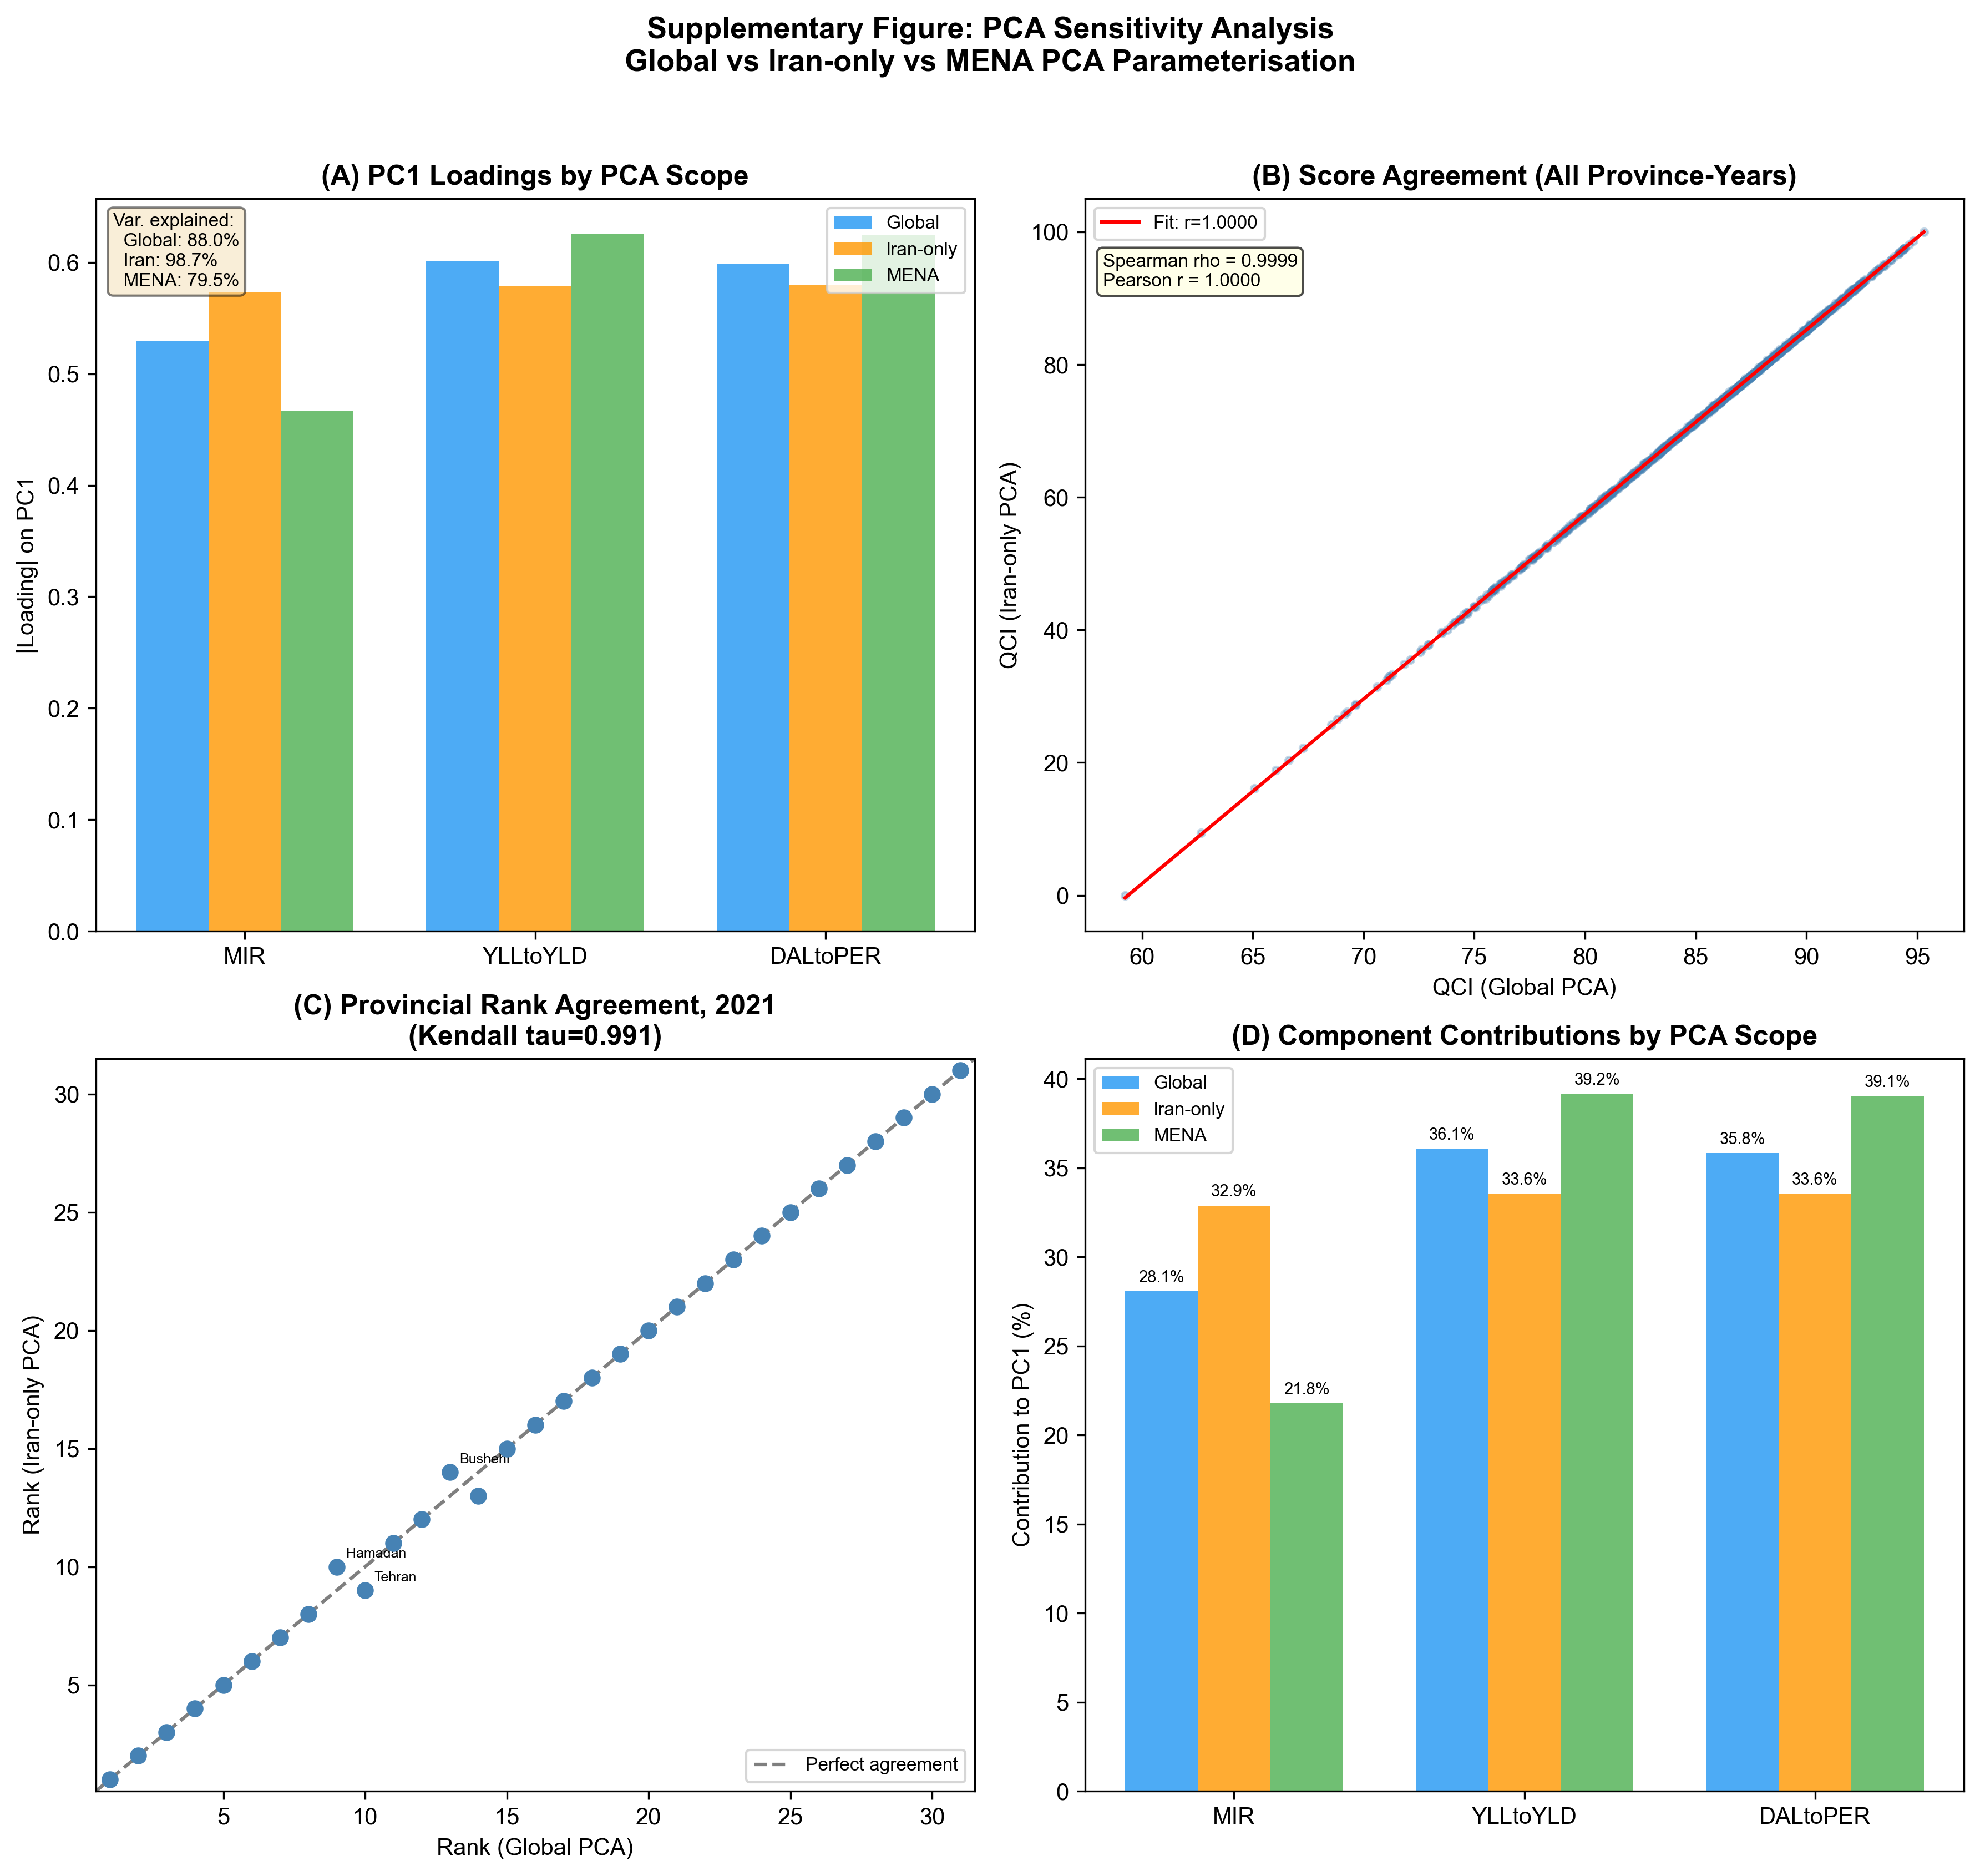
\includegraphics[width=\textwidth]{figure_supp_pca_sensitivity.png}
\caption*{\textbf{Supplementary Figure S1.} PCA sensitivity analysis comparing global, Iran-only, and MENA parameterisations. (A) Absolute PC1 loadings by PCA scope, with variance explained. (B) QCI score agreement between global and Iran-only PCA across all 992 province-year observations (Spearman $\rho = 0.9999$). (C) Provincial rank agreement in 2021 (Kendall's $\tau = 0.991$); 27 of 31 provinces have identical rankings. (D) Squared loading contributions showing the relative importance of each component under each PCA scope. The near-perfect concordance confirms that the globally-derived PCA parameterisation is appropriate for the Iran subnational analysis.}
\end{figure}

\clearpage

\begin{table}[htbp]
\centering
\caption*{\textbf{Supplementary Table S1.} Provincial QCI ranking comparison, 2021: global PCA vs Iran-only PCA vs MENA PCA parameterisation. All 31 provinces shown, sorted by global PCA rank.}
\small
\begin{tabular}{lcccccc}
\toprule
 & \multicolumn{2}{c}{Global PCA} & \multicolumn{2}{c}{Iran-only PCA} & Rank & MENA \\
\cmidrule(lr){2-3} \cmidrule(lr){4-5}
Province & QCI & Rank & QCI & Rank & Diff. & Rank \\
\midrule
Chahar Mahaal \& Bakhtiari & 98.77 & 1 & 100.00 & 1 & 0 & 1 \\
Kohgiluyeh \& Boyer-Ahmad & 98.32 & 2 & 95.37 & 2 & 0 & 2 \\
Fars & 98.27 & 3 & 94.89 & 3 & 0 & 3 \\
Isfahan & 98.26 & 4 & 94.82 & 4 & 0 & 4 \\
Kermanshah & 98.07 & 5 & 92.79 & 5 & 0 & 5 \\
Kurdistan & 97.98 & 6 & 91.91 & 6 & 0 & 6 \\
Qazvin & 97.98 & 7 & 91.88 & 7 & 0 & 9 \\
Mazandaran & 97.96 & 8 & 91.73 & 8 & 0 & 8 \\
Hamadan & 97.94 & 9 & 91.55 & 10 & 1 & 10 \\
Tehran & 97.94 & 10 & 91.57 & 9 & 1 & 7 \\
Ilam & 97.87 & 11 & 90.85 & 11 & 0 & 11 \\
Zanjan & 97.85 & 12 & 90.62 & 12 & 0 & 12 \\
Bushehr & 97.66 & 13 & 88.58 & 14 & 1 & 14 \\
Markazi & 97.66 & 14 & 88.73 & 13 & 1 & 13 \\
Ardebil & 97.64 & 15 & 88.42 & 15 & 0 & 15 \\
\multicolumn{7}{c}{\dots} \\
Sistan \& Baluchistan & 95.20 & 31 & 62.49 & 31 & 0 & 31 \\
\midrule
\multicolumn{3}{l}{\textbf{Cosine similarity (loadings)}} & \multicolumn{2}{c}{0.999} & & 0.997 \\
\multicolumn{3}{l}{\textbf{Pearson $r$ (scores)}} & \multicolumn{2}{c}{0.9999} & & 0.9999 \\
\multicolumn{3}{l}{\textbf{Kendall's $\tau$ (ranks, 2021)}} & \multicolumn{2}{c}{0.991} & & 0.974 \\
\bottomrule
\end{tabular}

\vspace{0.5em}
\noindent\small Rank Diff. = absolute difference in rank between global and Iran-only PCA. Maximum rank difference = 1 position. Iran-only QCI scores use a different 0--100 scale (Iran-specific min--max normalisation), hence absolute values differ while relative rankings are preserved.
\end{table}

\end{document}
